% Se incluye el preambulo del trabajo
% Se configura el tipo de documento
\documentclass[a4paper]{scrartcl}

%THIS IS TO MAKE THE DOCUMENT PRETTIER
\usepackage[utf8]{inputenc}
\usepackage[spanish, es-tabla, es-nodecimaldot]{babel}

\usepackage[T1]{fontenc}
\usepackage{lmodern} %AGREGO1
\usepackage{fourier}			% English language/hyphenation

\usepackage{color}
\usepackage[protrusion=true,expansion=true]{microtype}
\usepackage{amsmath}
\usepackage{amsfonts,amsthm} % Math packages
\usepackage[pdftex]{graphicx}
\usepackage{url}
\usepackage{import}
\usepackage{multicol}

\usepackage[margin=2cm]{geometry}

% %%% Custom sectioning
\usepackage{sectsty}
\allsectionsfont{\normalfont \scshape}

%%% Custom headers/footers (fancyhdr package)
\usepackage{fancyhdr}
\pagestyle{fancyplain}

\fancyhead{}											% No page header
\fancyfoot[L]{}											% Empty
\fancyfoot[C]{}											% Empty
\fancyfoot[R]{\thepage}									% Pagenumbering
\renewcommand{\headrulewidth}{0pt}			% Remove header underlines
\renewcommand{\footrulewidth}{0pt}				% Remove footer underlines
\setlength{\headheight}{13.6pt}

%%% Equation and float numbering
\numberwithin{equation}{section}		% Equationnumbering: section.eq#
\numberwithin{figure}{section}			% Figurenumbering: section.fig#
\numberwithin{table}{section}				% Tablenumbering: section.tab#

%%% Maketitle metadata
\newcommand{\horrule}[1]{\rule{\linewidth}{#1}} 	% Horizontal rule
%FINISHED MAKING PRETTIER DOCUMENT



% --------------ADDED BY FACUNDO FARALL--------------

%MATHEMATICS PACKAGES
\usepackage{amsmath,amsfonts,amsthm}
%FINISHED MATHEMATICS



%THIS IS FOR SETTING LOCATION OF FLOATS
\usepackage{float}
%ENDS SETTING LOCATION OF FLOATS



%THIS IS SO THAT REFERENCES CAN BE CLICKED
\usepackage{hyperref}
\hypersetup{
    colorlinks=true,
    linkcolor=blue,
    filecolor=magenta,      
    urlcolor=blue,
    citecolor=blue,    
}
%FINISHED CLICKABLE REFERENCES



%THIS IS TO CHANGE MARGINES FOR SITUATIONS LIKE LONG EQUATIONS
\usepackage[strict]{changepage}
%ENDS CHANGER OF MARGINS



%THIS IS TO USE SMALLER FONT SIZE
\usepackage[11pt]{moresize}
%FINISHED FONT SIZE CHANGER



%THE FOLLOWING ARE CONFIGURATIONS FOR TODONOTES
\usepackage{todonotes,varwidth}
\makeatletter
\tikzstyle{diaanotestyle} = [
    draw=\@todonotes@currentbordercolor,
    fill=\@todonotes@currentbackgroundcolor,
    line width=0.5pt,
    inner sep = 0.8 ex,
    rounded corners=4pt,align=left,
   ]

\renewcommand{\@todonotes@drawInlineNote}{%
        {\begin{tikzpicture}[remember picture,baseline={(0,0)}]%
            \draw node[diaanotestyle,font=\@todonotes@sizecommand,anchor=base west]{%
               \begin{varwidth}[t]{10cm}
                \if@todonotes@authorgiven%
                    {\@todonotes@sizecommand \@todonotes@author:\,\@todonotes@text}%
                \else%
                    {\@todonotes@sizecommand \@todonotes@text}%
                \fi
                \end{varwidth}};%
            \end{tikzpicture}}%
       }%
\makeatother
%HERE ENDS THE CONFIGURATIONS FOR TODONOTES

% --------------ENDS ADDED BY FACUNDO FARALL--------------



% Se agrega el titulo o caratula del trabajo

% Se crea el documento y agregan los ejercicios
\begin{document}

	% Crear y configurar el titulo/caratula del informe
	\title{
		\normalfont \normalsize \textsc{Instituto Tecnol\'ogico de Buenos Aires} \\ [25pt]
		\huge Trabajo Pr\'actico N$^{\circ}$3 \\
		\author{
			\\Grupo 1:\\\\Farall, Facundo David\\Gaytan, Joaqu\'in Oscar\\Kammann, Lucas\\Maselli, Carlos Javier\\M\"uller, Malena \\ \\ \\ \\
			Profesores: \\\\ Cossutta, Pablo Mart\'in\\Weill, Mar\'ia Alejandra\\Salvati, Mat\'ias Dami\'an \\ \\ \\ 
		} 		
		\text{Teor\'ia de los Circuitos - 2019}
	}
	\pagenumbering{arabic}
	\maketitle
	\newpage

	% Se agrega el indice con el contenido del trabajo
	\tableofcontents

	\newpage
	
\section{Filtro High Pass Notch}

A continuaci\'on se estudia la implementaci\'on de un filtro mediante el circuito de la figura \ref{circ1}. Si bien una parte del circuito parecer\'ia ser un GIC, debido a la presencia de la resistencia R8 no lo es.

\begin{figure}[H] %!ht
	\centering
	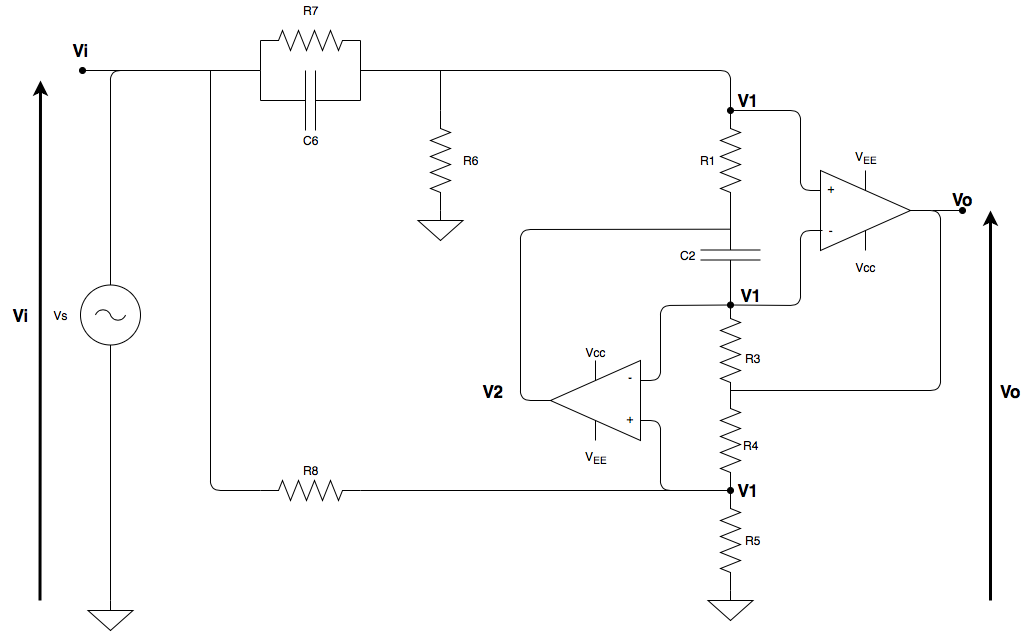
\includegraphics[scale=0.4]{../EJ1/circuito1.png}
	%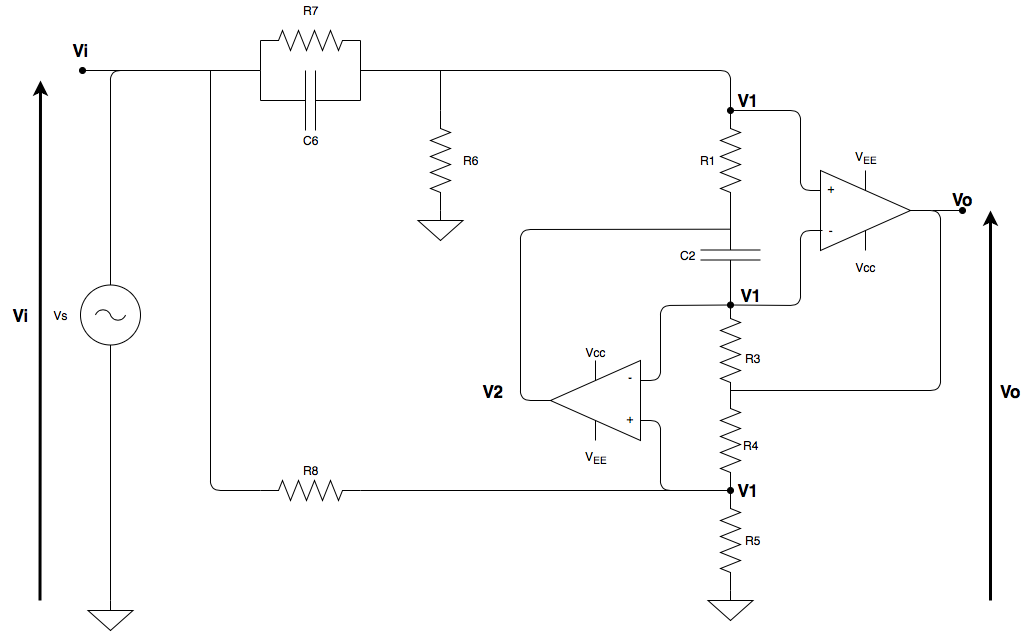
\includegraphics[width=10cm,height=10cm,keepaspectratio]{../EJ1/circuito1.png}
	\caption{Circuito empleado como filtro, involucrando una configuraci\'on similar a un GIC.}
	\label{circ1}
\end{figure}

Los opamps empleados para este circuito son LM833\footnote{Hoja de datos del operacional LM833: https://html.alldatasheet.com/html-pdf/784648/TI1/LM833/52/1/LM833.html}. ya que tienen un slew rate alto ($7V/\mu s$) y un GBP de 16MHz, lo cual permitir\'ia operar correctamente hasta las frecuencias de MHz alcanzadas con los generadores de se\~nales del laboratorio de la facultad.

\subsection{Funci\'on transferencia del circuito}
Debido a la complejidad del circuito \ref{circ1}, se  calcul\'o $\frac{V_O}{V_I}$ considerando a los dos amplificadores operacionales como ideales. Esto implica que se haya considerado $A_{vol}$ infinito. Para este an\'alisis, mediante resoluci\'on por nodos, se parti\'o de las relaciones entre corrientes entranes y salientes a cada uno de los tres nodos indicados en el circuito con tensi\'on $V_1$:

\begin{equation}
\begin{cases}
\frac{V_i - V_1}{(R_7 // \frac{1}{sC_6})} = \frac{V_1}{R_6} + \frac{V_1 - V_2}{R_1}\\ \\
\frac{V_2 - V_1}{\frac{1}{sC_2}} = \frac{V_1 - V_O}{R_3}\\ \\
\frac{V_O - V_1}{R_4} = \frac{V_1 - V_i}{R_8} + \frac{V_1}{R_5}
\end{cases}
\label{ecsbase}
\end{equation}

Operando algebraicamente, a partir de las ecuaciones \ref{ecsbase} se obtiene la funci\'on transferencia del circuito \ref{circ1}. Siendo $s = j\omega$, la misma se muestra a continuaci\'on:

\begin{equation}
H(s) = \frac{V_O}{V_I} = \frac{R_4 + R_5}{R_5} \cdot 
\frac
{ s^2
	+\frac{R_4 R_6 R_8 + R_5 R_6 R_8 - R_4 R_5 R_7}{C_6 R_6 R_7 R_8 (R_4 + R_5)} \cdot s
	+\frac{R_4 R_5}{C_2 C_6 R_1 R_3 R_8 (R_4 + R_5)}}
{s^2
	+\frac{R_6 + R_7}{C_6 R_6 R_7} \cdot s
	+\frac{R_4 (R_5 + R_8)}{C_2 C_6 R_1 R_3 R_5 R_8}
}
\label{vovi}
\end{equation}


\subsubsection{Caracter\'sticas del circuito a partir de la funci\'on transferencia}

Si bien observando la funci\'on transferencia se puede decir que se trata de un filtro de segundo orden, a continuaci\'on se analiza m\'as en detalle a qu\'e tipo de filtro corresponde.

\paragraph*{Polos y ceros:}
A partir del t\'ermino de grado cero del numerador y del denominador del cociente de polinomios de la expresi\'on de $H(s)$ (Ecuaci\'on \ref{vovi}) se puede obtener la expresi\'on de los polos y ceros del circuito, ya que simb\'olicamente dichos t\'erminos son $\left(\frac{s}{\omega_Z}\right)^2$ y $\left(\frac{s}{\omega_P}\right)^2$respectivamente. Por lo tanto,

\begin{equation}
\omega_Z = \sqrt{\frac{R_4 R_5}{C_2 C_6 R_1 R_3 R_8 (R_4 + R_5)}}
\label{ec_z}
\end{equation}

\begin{equation}
\omega_P = \sqrt{\frac{R_4 (R_5 + R_8)}{C_2 C_6 R_1 R_3 R_5 R_8}}
\label{ec_p}
\end{equation}

Observando las diferencias entre los numeradores de las expresiones \ref{ec_z} y \ref{ec_p} se puede ver que como $R_5 < R_5 + 5_8$, el numerador del $\omega_Z$ es menor que el de $\omega_P$. Analizando los denominadores de igual manera, se v\'e que el denominador de $\omega_Z$ es mayor al denominador de $\omega_P$ ya que $R_4 + R_5 > R_5$. Por lo tanto, $\omega_Z < \omega_P$. Esto indica que el circuito \ref{circ1} es un filtro $High-Pass$ $ Notch$.


\paragraph*{Ganancia del circuito (G):}  La ganancia $G$ para el caso de un filtro $High-Pass$ $ Notch$ se obtiene como $\lim_{s\to\infty}H(s)$, estando $H(S)$ definida por la expresi\'on \ref{vovi} y as\'i es como resulta:
\begin{equation}
G = \lim_{s\to\infty}H(s) = 1 + \frac{R_4}{R_5} 
\label{G}
\end{equation}

\paragraph*{Factor de calidad (Q):} El coeficinete que acompa\~na a "s" en el denominador de la expresi\'on \ref{vovi} es $\frac{\omega_P}{Q}$. Por lo tanto, a partir de dicho coeficiente y de la expresi'on \ref{ec_p} correspondiente al $\omega_P$, se obtiene que:

\begin{equation}
Q = \frac{R_{6} R_{7}}{R_{6} + R_{7}} \cdot \sqrt{\frac{C_{6} R_{4} \left(R_{5} + R_{8}\right)}{C_{2} R_{1} R_{3}R_{5} R_{8} }}
\end{equation}


\subsection{An\'alisis de sensibilidades}

Para dicho an\'alisis se prosigui\'o mediante la ecuaci\'on \ref{sens}, siendo $X$ el valor de un componente e $Y$ el par\'ametro del circuito cuya sensibilidad respecto a $X$ se quiere calcular.

\begin{equation}
S^{Y}_{X}= \lim_{\Delta X \to \infty} \left(\frac{\Delta Y / Y}{\Delta X / X}\right) = \frac{X}{Y}\cdot\frac{dY}{dX}
\label{sens}
\end{equation}

Los par\'ametros sobre los que se analiz\'o la sensibilidad de cada uno de los componentes son $\omega_Z$, $\omega_P$ y $Q$. Sus resultados fueron los siguientes:

Sensibilidades de $\omega_Z$ respecto a cada componente del circuito:
\begin{equation}
\begin{cases}
S^{\omega_Z}_{R_4}= \frac{1}{2} \cdot \frac{R_{5}}{R_{4} + R_{5}}\\ \\
S^{\omega_Z}_{R_5}= \frac{1}{2} \cdot \frac{R_{4}}{R_{4} + R_{5}}\\ \\
S^{\omega_Z}_{C_2} = S^{\omega_Z}_{C_6}= S^{\omega_Z}_{R_1}=S^{\omega_Z}_{R_3}=S^{\omega_Z}_{R_8}    =- \frac{1}{2} 
\end{cases}
\end{equation}

Sensibilidades de $\omega_P$ respecto a cada componente del circuito:
\begin{equation}
\begin{cases}
S^{\omega_P}_{R_5} =	-  \frac{1}{2} \cdot \frac{R_{8}}{R_{5} + R_{8}} \\ \\
S^{\omega_P}_{R_8} =	-  \frac{1}{2} \cdot \frac{R_{5}}{R_{5} + R_{8}}\\ \\
S^{\omega_P}_{C_2} = S^{\omega_P}_{C_6}= S^{\omega_P}_{R_1}=S^{\omega_P}_{R_3}=	-  \frac{1}{2}\\ \\
S^{\omega_P}_{R_4} = \frac{1}{2}
\end{cases}
\end{equation}

Sensibilidades de $Q$ respecto a cada componente del circuito:
\begin{equation}
\begin{cases}
S^{Q}_{R_6} = \frac{R_{7}}{R_{6} + R_{7}}\\ \\
S^{Q}_{R_7} = \frac{R_{6}}{R_{6} + R_{7}}\\ \\
S^{Q}_{R_5} = \frac{1}{2} \frac{(C_{2} R_{1} R_{3} R_{5} R_{8})^2 \left(C_{6} R_{4} R_{5} - 1\right)}{C_{6} R_{4} \left(R_{5} + R_{8}\right) \left(R_{6} + R_{7}\right)^{2}} \\ \\
S^{Q}_{R_8} = \frac{1}{2} \frac{(C_{2} R_{1} R_{3} R_{5} R_{8})^2 \left(C_{6} R_{4} R_{8} - 1\right)}{C_{6} R_{4} \left(R_{5} + R_{8}\right) \left(R_{6} + R_{7}\right)^{2}} \\ \\
S^{Q}_{C_6} = S^{Q}_{R_4} =\frac{1}{2} \\ \\
S^{Q}_{C_2} = S^{Q}_{R_1} = S^{Q}_{R_3} =-\frac{1}{2}
\end{cases}
\end{equation}

A partir de las expresiones de las sensibilidades se puede decir que en caso de querer variar $\omega_Z$ lo conveniente es modificando $C_2$, $C_6$, $R_1$, $R_3$ o $R_8$ ya que tienen valores constantes. Al modificar el $\omega_Z$ , uno puede desplazar la frecuencia a la cual se encuentra el pico del Notch, ya que dicho pico se debe al Q grande del cero, y a la ubicaci\'on de dicho cero. Para el $\omega_P$ lo conveniente es variar $C_2$, $C_6$, $R_1$, $R_3$ o $R_4$. Y finalmente para el Q los mejores componentes de ajuste al valor deseado son $C_6$, $R_4$, $C_2$, $R_1$ o $R_3$. En m\'odulo todas presentan el mismo valor y al no depender de los valores de otros componentes, permiten hacer mejor un ajuste. 

\subsection{Dise\~no del circuito - Selecci\'on de componentes}
Para elegir los valores de cada uno de los componentes del circuito, se tuvieron en cuenta las sugerencias indicadas en el enunciado del trabajo pr\'actico.

\begin{itemize}
	\item $R_1 = R_3 = R_8 = R$
	\item $R_6 = (1 + k^2) Q R$
	\item $R_7 = (1 + \frac{1}{k^2})Q R$
	\item $R_4 = \frac{2k^2}{1+k^2}R$
	\item $R_5 = \frac{2k^2}{1-k^2}R$
	\item $C_2 = C_6 = C$
	\item $k = \frac{\omega_Z}{\omega_P} \leqslant 1 $
\end{itemize}

Reemplazando con los valores de las sugerencias previamente mencionadas, se reescribe la funci\'on transferencia de la ecuaci\'on \ref{vovi} para mayor simplicidad:

\begin{equation}
H(s) = \frac{2}{1+k^2} \cdot \frac{s^2 + \left( \frac{k}{RC}\right)^2}{s^2 + \frac{1}{RCQ} s + \left(\frac{1}{RC}\right)^2}
\label{vovi_simple}
\end{equation}

\begin{equation}
\frac{\omega_Z}{\omega_P} = k
\end{equation}

La siguiente tabla presenta las especificaciones consideradas para el dise\~no del circuito:

\begin{table}[h!]
	\centering
	\begin{tabular}{c c c}%
		\bfseries $\omega_P$ & Q & $|H(\infty)| (dB)$ \\ \hline
		$13000 \frac{rad}{s}$ & $2$ & $4dB$\\
		\hline
	\end{tabular}
	\caption{Especificaciones de dise\~no}
	\label{especificaciones}
\end{table}

A partir de la ecuaci\'on \ref{vovi_simple} y considerando lo indicado en la tabla \ref{especificaciones}:

\begin{equation}
\omega_P = \frac{1}{RC} = 13000\frac{rad}{s}
\label{dwp}
\end{equation}

Eligiendo $C = 100nF$, el valor de R debe ser tal que cumpla con la ecuaci\'on \ref{dwp}. Entonces $R = \frac{1}{13000 * 100 *10^{-9}} \approx 769\Omega.$ Por lo tanto tomamos el valor comercial m\'as cercano: $750\Omega$. Esto produce un $\omega_P = 13333 \frac{rad}{s}$. A partir de estos $C$ y $R$ elegidos, a continuaci\'on se muestran los valores que deb\'ian conseguirse para el resto de los componentes con la finalidad de respetar las especificaciones presentadas en la tabla \ref{especificaciones}.

\begin{table}[H]
	\centering
	\begin{tabular}{c c c c}%
		\bfseries  & Valor deseado & Valor obtenido& Componentes empleados \\ \hline
		$R4$ & $309,62\Omega$  & $309,52\Omega$ & $390\Omega // 1,5k\Omega$\\
		$R5$ & $527,3\Omega$  & $527,50\Omega$ & $1,2k\Omega // 1,2k\Omega$\\
		$R6$ & $1,89k\Omega$  & $1,89\Omega$ & $3k\Omega // 5,1k\Omega$\\
		$R7$ & $7,27k\Omega$  & $7,10k\Omega$ & $20k\Omega // 11k\Omega$\\
		\hline
	\end{tabular}
	\caption{Especificaciones de dise\~no}
	\label{especificaciones}
\end{table}

Es as\'i como se obtiene la funci\'on transferencia que se muestra a continuaci\'on:

\begin{equation}
H(s) = 1,59 \cdot \frac{s^2+73,52 \cdot 10^6}{1,26 s^2 + 6666,6 s + 177,78 \cdot 10^6}
\label{vovi_val}
\end{equation}


\subsection{Polos y ceros}

Anal\'iticamente se obtienen las siguientes expresiones para los polos y ceros del filtro:

\begin{equation}
s_{z1,z2} = - \frac{R_4  R_6  R_8+R_5  R_6  R_8 - R_4 R_5 R_7}{C_6 R_6 R_7 R_8 \cdot (R_4 + R_5)} \pm \sqrt{\left( \frac{R_4 R_6 R_8 + R_4 R_6 R_8 - R_4 R_5 R_7}{C_6 R_6 R_7 R_8 \cdot (R_4 + R_5)}\right)^2- 4 \cdot \frac{R_4 R_5}{C_2 C_6 R_1 R_3 R_8 \cdot (R_4 + R_5)}}
\label{ceros}
\end{equation}

\begin{equation}
s_{p1,p2} = - \frac{R_6 + R_7}{C_6 R_6 R_7} \pm \sqrt{\left( \frac{R_6 + R_7}{C_6 R_6 R_7}\right)^2 - 4 \cdot \frac{R_4(R_5+R_8)}{C_2 C_6 R_1 R_3 R_5 R_8}}
\label{polos}
\end{equation}


A partir de las expresiones anteriores, al reemplazar con los valores de los componentes empleados, se obtiene el siguiente diagrama de polos y ceros del filtro high pass notch, con $Q\approx 2$:

\begin{figure}[H] %!ht
	\centering
	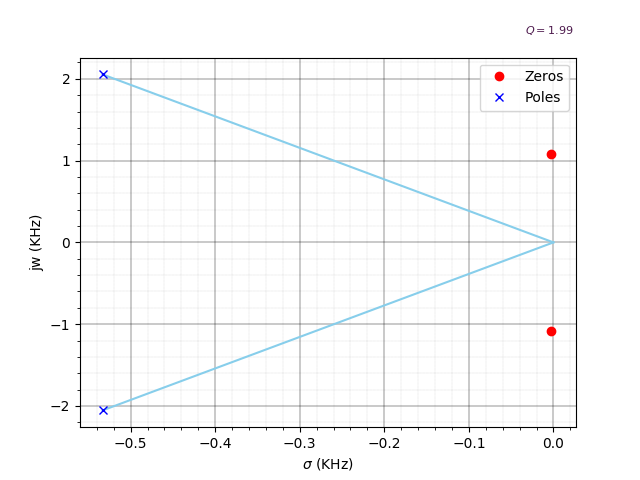
\includegraphics[width=10cm,height=10cm,keepaspectratio]{../EJ1/00GRAFICOS/singularidades.png}
	\caption{Polos y ceros de la funci\'on transferencia del circuito.}
	\label{c1vinmax}
\end{figure}

Los polos se encuentran claramente del lado izquierdo del eje $j\omega$, lo que indica estabilidad del circuito.


\subsection{Variaci\'on de la resistencia $R_8$}

\paragraph*{Influencia en la funci\'on transferencia:} A continuaci\'on se muestra la funci\'on transferencia del circuito, con $R_8\to 0$ y luego con $R_8\to \infty$. Para ambos casos se obtiene la expresi\'on en funci\'on del resto de los componentes del circuito y se agrega el resultado luego de reemplazar dichas expresiones con los valores de los componentes empleados (indicados en la tabla \ref{componentes}.

\begin{equation}
\lim_{R_8\to 0} H(s) = - \frac{R_4 + R_5}{R_5} \cdot 
\left(\frac{C_2 C_6 R_1 R_3 R_5 R_7}{C_6 R_6 R_7(R_4 + R_5)+\frac{R_4 R_5}{C_2 C_6 R_1 R_3 (R_4+R_5)}}\right)s = - 9.63 \cdot 10^{-13} s
\end{equation}

\begin{equation}
\lim_{R_8\to \infty} H(s) = \frac{R_4 + R_5}{R_5} \cdot \frac{s^2 + \frac{1}{C_6 R_7}s}{s^2 + \frac{R_6 + R_7}{C_6 R_6 R_7}\cdot s + \frac{R_4}{C_2 C_6 R_1 R_3 R_5}} = \frac{1.59 s^{2} + 4473.45}{s^{2} + 6699.83 s + 104,39 \cdot 10^6}
\end{equation}

Se pueden ver en el siguiente gr\'afico la funci\'on transferencia para estos dos casos.

\begin{figure}[H] %!ht
	\centering
	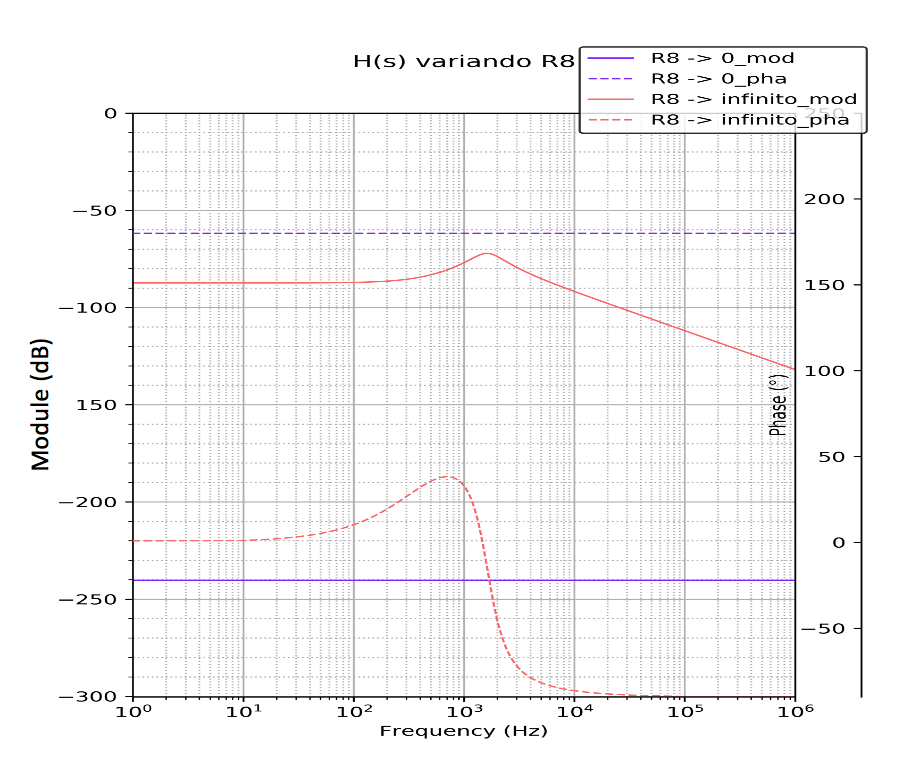
\includegraphics[width=10cm,height=10cm,keepaspectratio]{../EJ1/00GRAFICOS/r88.png}
	\caption{H(s) con $R_8 \to 0$ y $R_8 \to \infty$}
	\label{r8}
\end{figure}

Mirando la ganancia en el gr\'afico \ref{r8}, es facil notar que el valor de la resistencia $R_8$ es fundamental para el filtro high pass notch, ya que cortocircuitandola o abriendo el circuito en su lugar, el comportamiento del circuito es completamente distinto.

\subsection{Variaci\'on de la resistencia $R_6$}

A continuaci\'on se muestra c\'omo cambian los polos y ceros al modificar la resistencia $R_6$ en la expresi\'on de la transferencia \ref{vovi}, dejando fijas las otras resistencias y los capacitores con los valores determinados para implementar el filtro.


\begin{figure}[H] %!ht
	\centering
	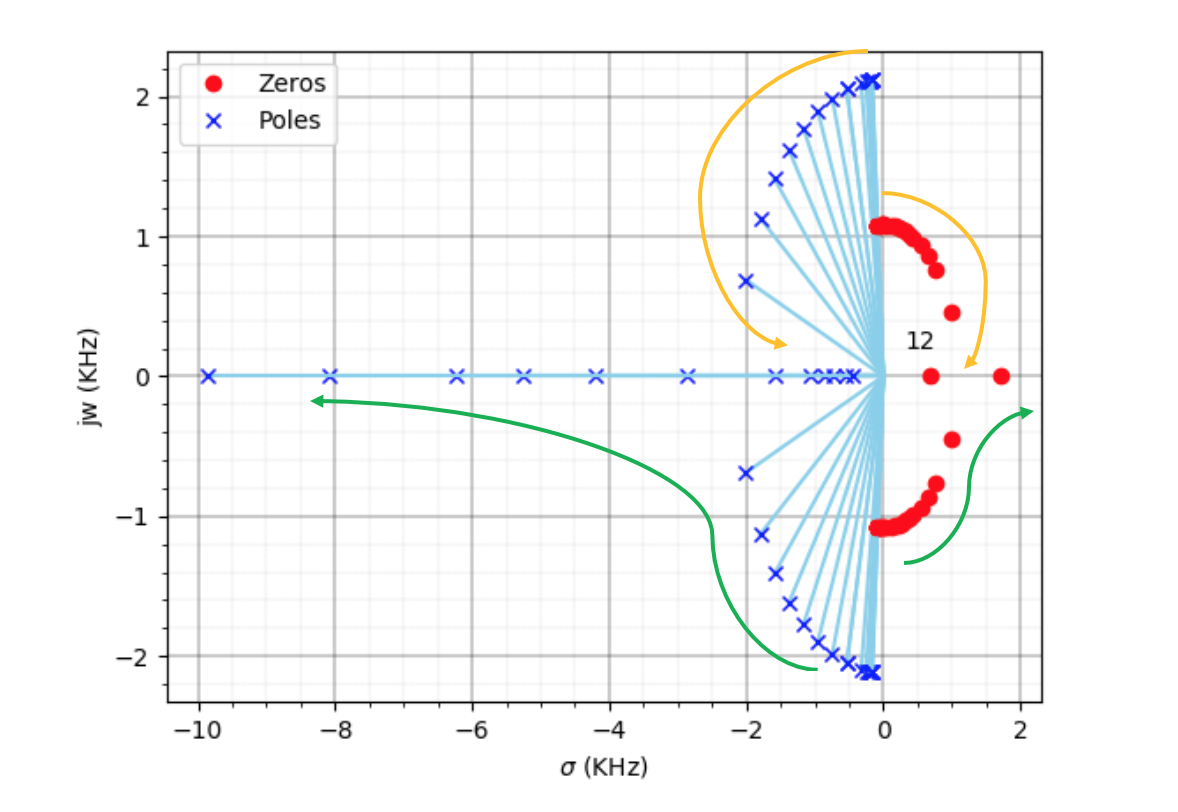
\includegraphics[width=10cm,height=10cm,keepaspectratio]{../EJ1/00GRAFICOS/r6.png}
	\caption{Polos y ceros del circuito al variar $R_6$}
	\label{r6}
\end{figure}

En la figura \ref{r6} se indica con flechas hacia donde tienden los polos y los ceros al hacer tender R6 a cero. Las flechas amarillas corresponden a la variaci\'on del polo $P1$ y del cero $Z1$ en dicho caso, mientras que las flechas verdes indican el comportamiento del polo $P2$ y del cero $Z2$. Para el caso en el que R6 tiende a infinito, las flechas van en sentido contrario al indicado en la figura. A continuaci\'on se muestran anal\'iticamente dichos comportamientos:

\begin{equation}
\lim_{R_6\to 0} s_{z1,z2} \approx \lim_{R_6\to 0}\left( \frac{R_4 R_5}{C_6 R_6 R_8} \pm \frac{R_4 R_5}{C_6 R_6 R_8}\right) \Rightarrow 
\begin{cases} 
s_{z1} \to +\infty\\
s_{z2} \to 0
\end{cases}
\end{equation}

\begin{equation}
\lim_{R_6\to 0} s_{p1,p2} \approx 	\lim_{R_6\to 0} \left( -\frac{R_6 + R_7}{C_6 R_6 R_7} \pm \frac{R_6 + R_7}{C_6 R_6 R_7} \right) \Rightarrow
\begin{cases} 
s_{p1} \to 0\\
s_{p2} \to -\infty
\end{cases}
\end{equation}

\begin{equation}
\lim_{R_6\to\infty}s_{z1,z2} =  -\frac{1}{C_6 R_7} \pm \sqrt{\left(\frac{1}{C_6 R_7} \right)^2 - 4 \cdot \frac{R_4 R_5}{C_2 C_6 R_1 R_3 R_8(R_4 + R_5)}}
\end{equation}

\begin{equation}
\lim_{R_6\to\infty}s_{p1,p2} =  - \frac{1}{C_6 R_7} \pm \sqrt{\left(\frac{1}{C_6 R_7}\right)^2 - 4 \cdot \frac{R_4 (R_5 + R_8)}{C_2 C_6 R_1 R_3 R_5 R_8 }}
\end{equation}



\subsection{Medici\'on de la transferencia del circuito}

Aqu\'i se compara la funci\'on transferencia del circuito te\'orica, 
medida y simulada mediante el m\'etodo de Montecarlo. Para la medici\'on se emple\'o el bodeador realizado para este trabajo. La simulaci\'on se llev\'o a cabo considerando tolerancias de $1\%$ para las resistencias ya que las empleadas fueron SMD y $10\%$ para los capacitores hole through. Adem\'as, se aclara que la simulaci\'on fue realizada incluyendo las impedancias equivalentes de $10M\Omega // 12pF$ aportadas por las puntas del osciloscopio que se usaron para tomar las mediciones.

\begin{figure}[H] %!ht
	\centering
	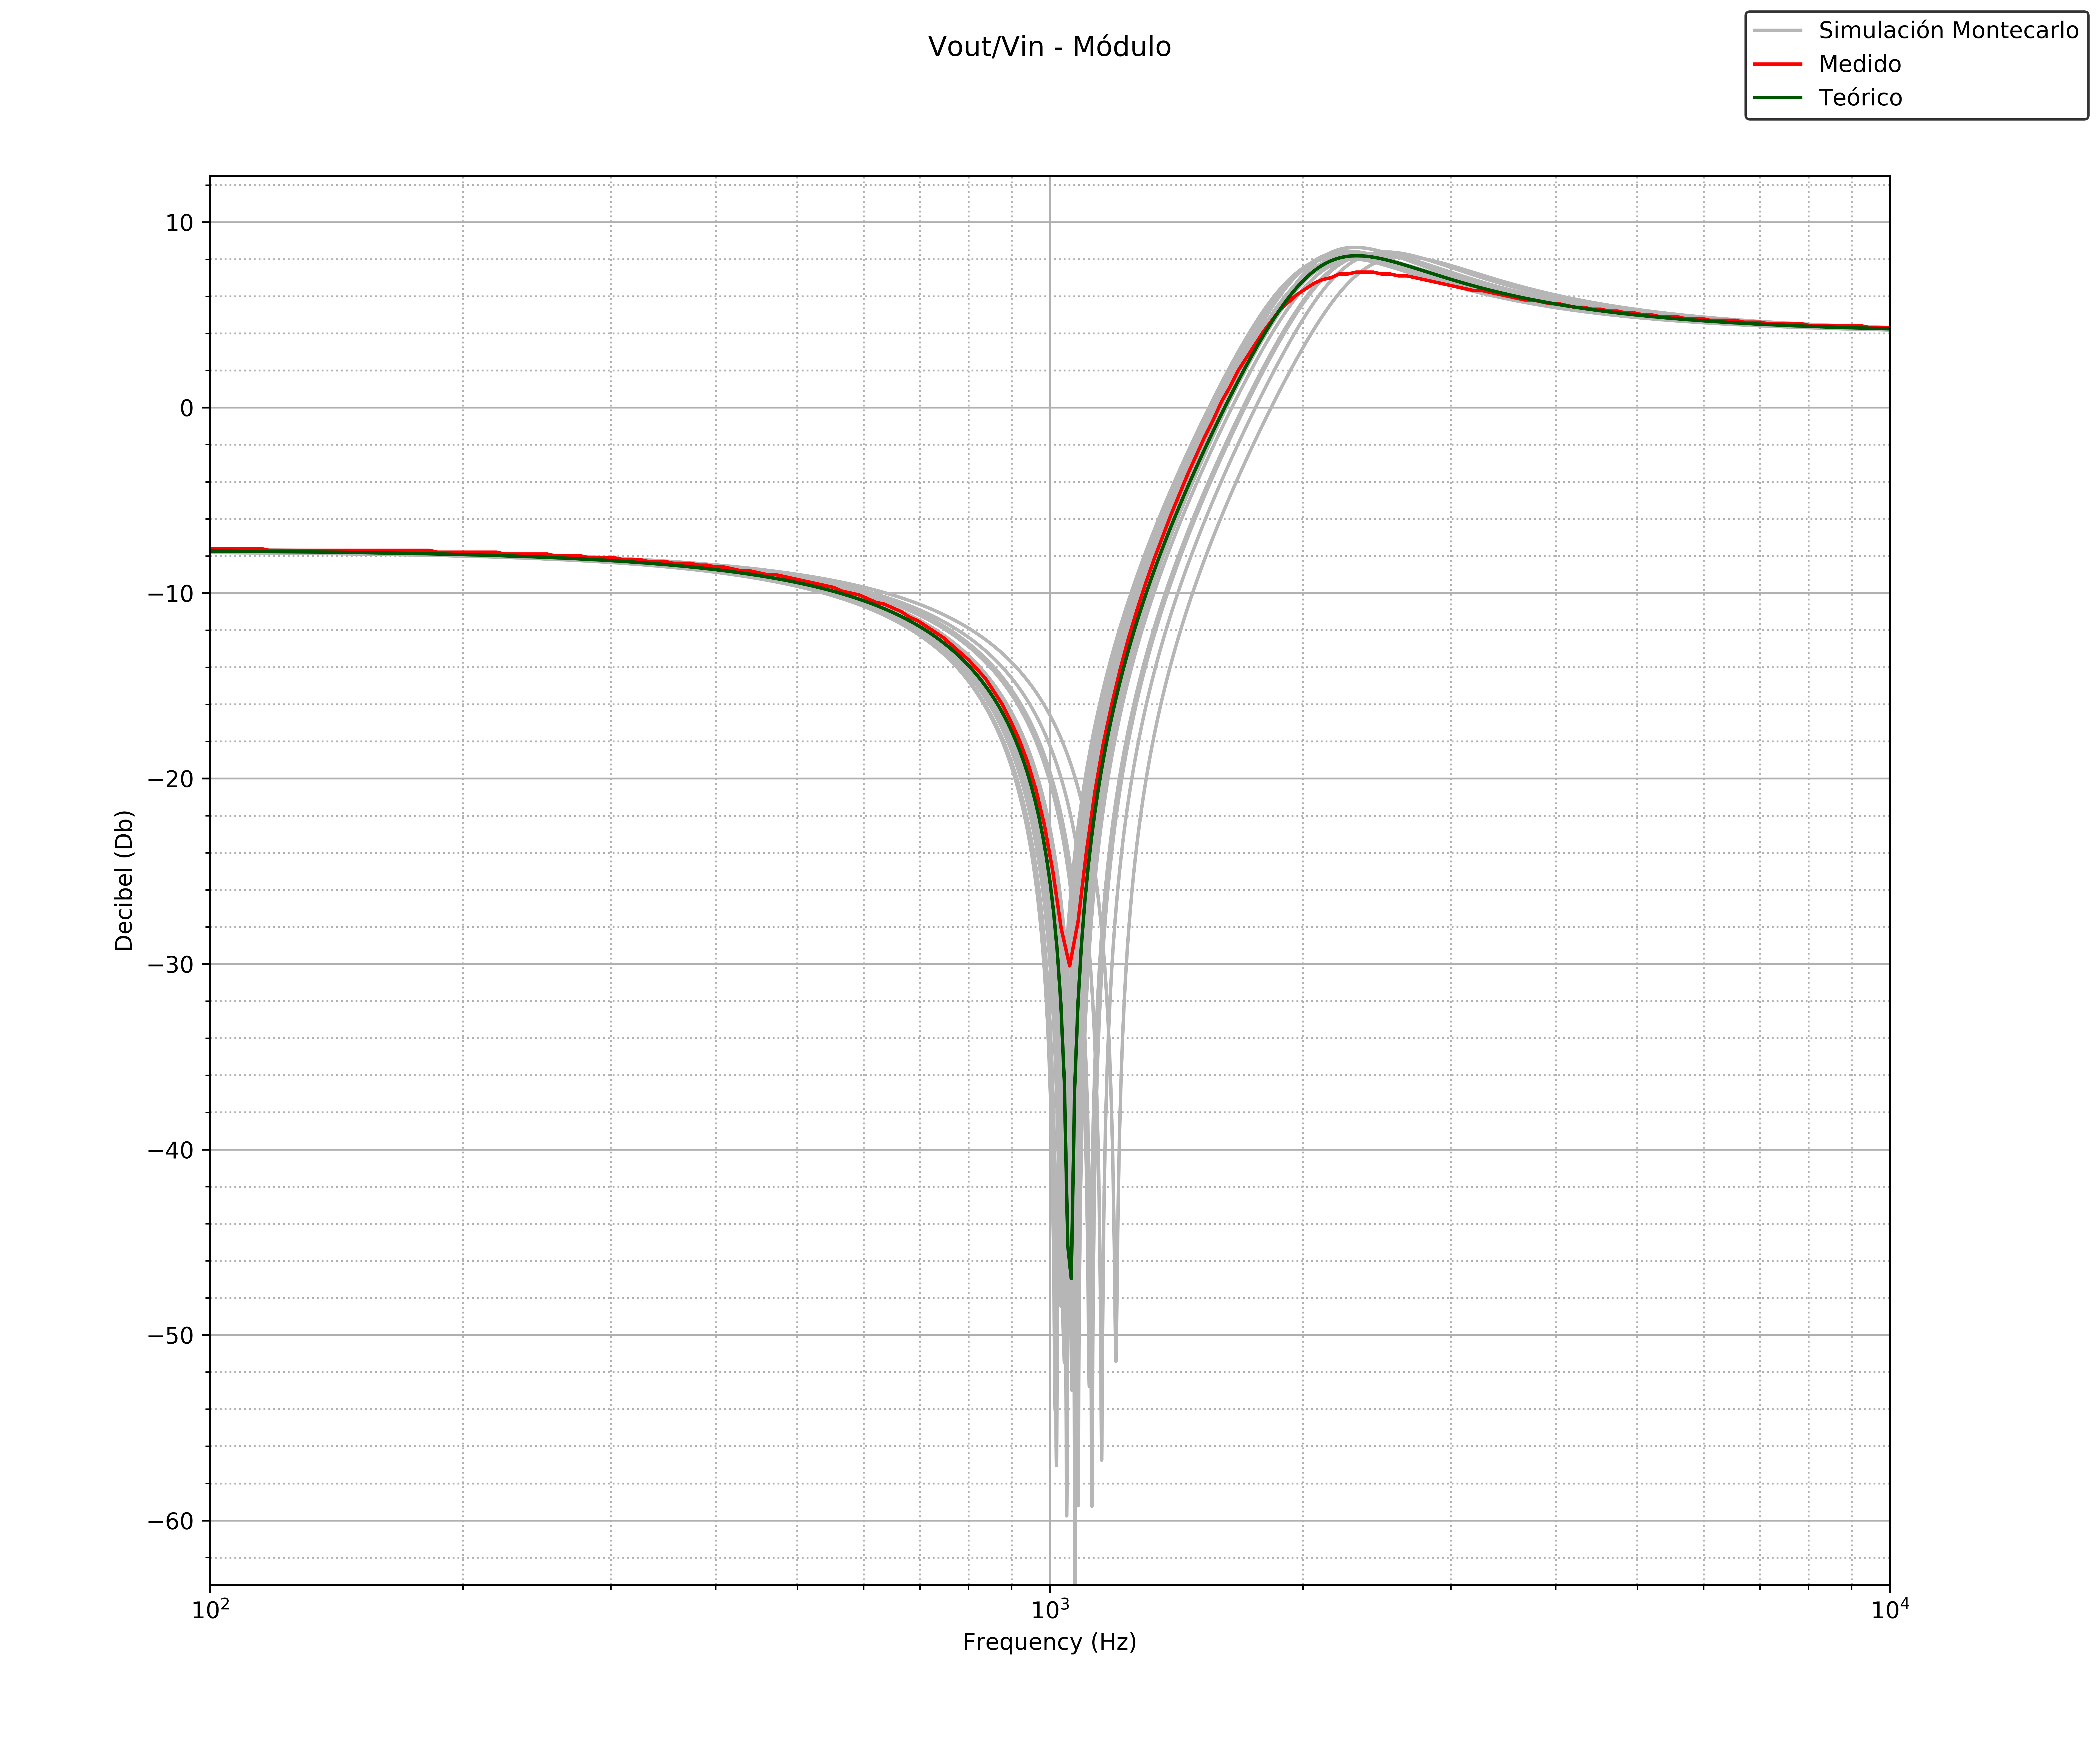
\includegraphics[width=10cm,height=10cm,keepaspectratio]{../EJ1/00GRAFICOS/vovi.png}
	\caption{M\'odulo de la transferencia del circuito.}
	\label{vovi_mod}
\end{figure}

\begin{figure}[H] %!ht
	\centering
	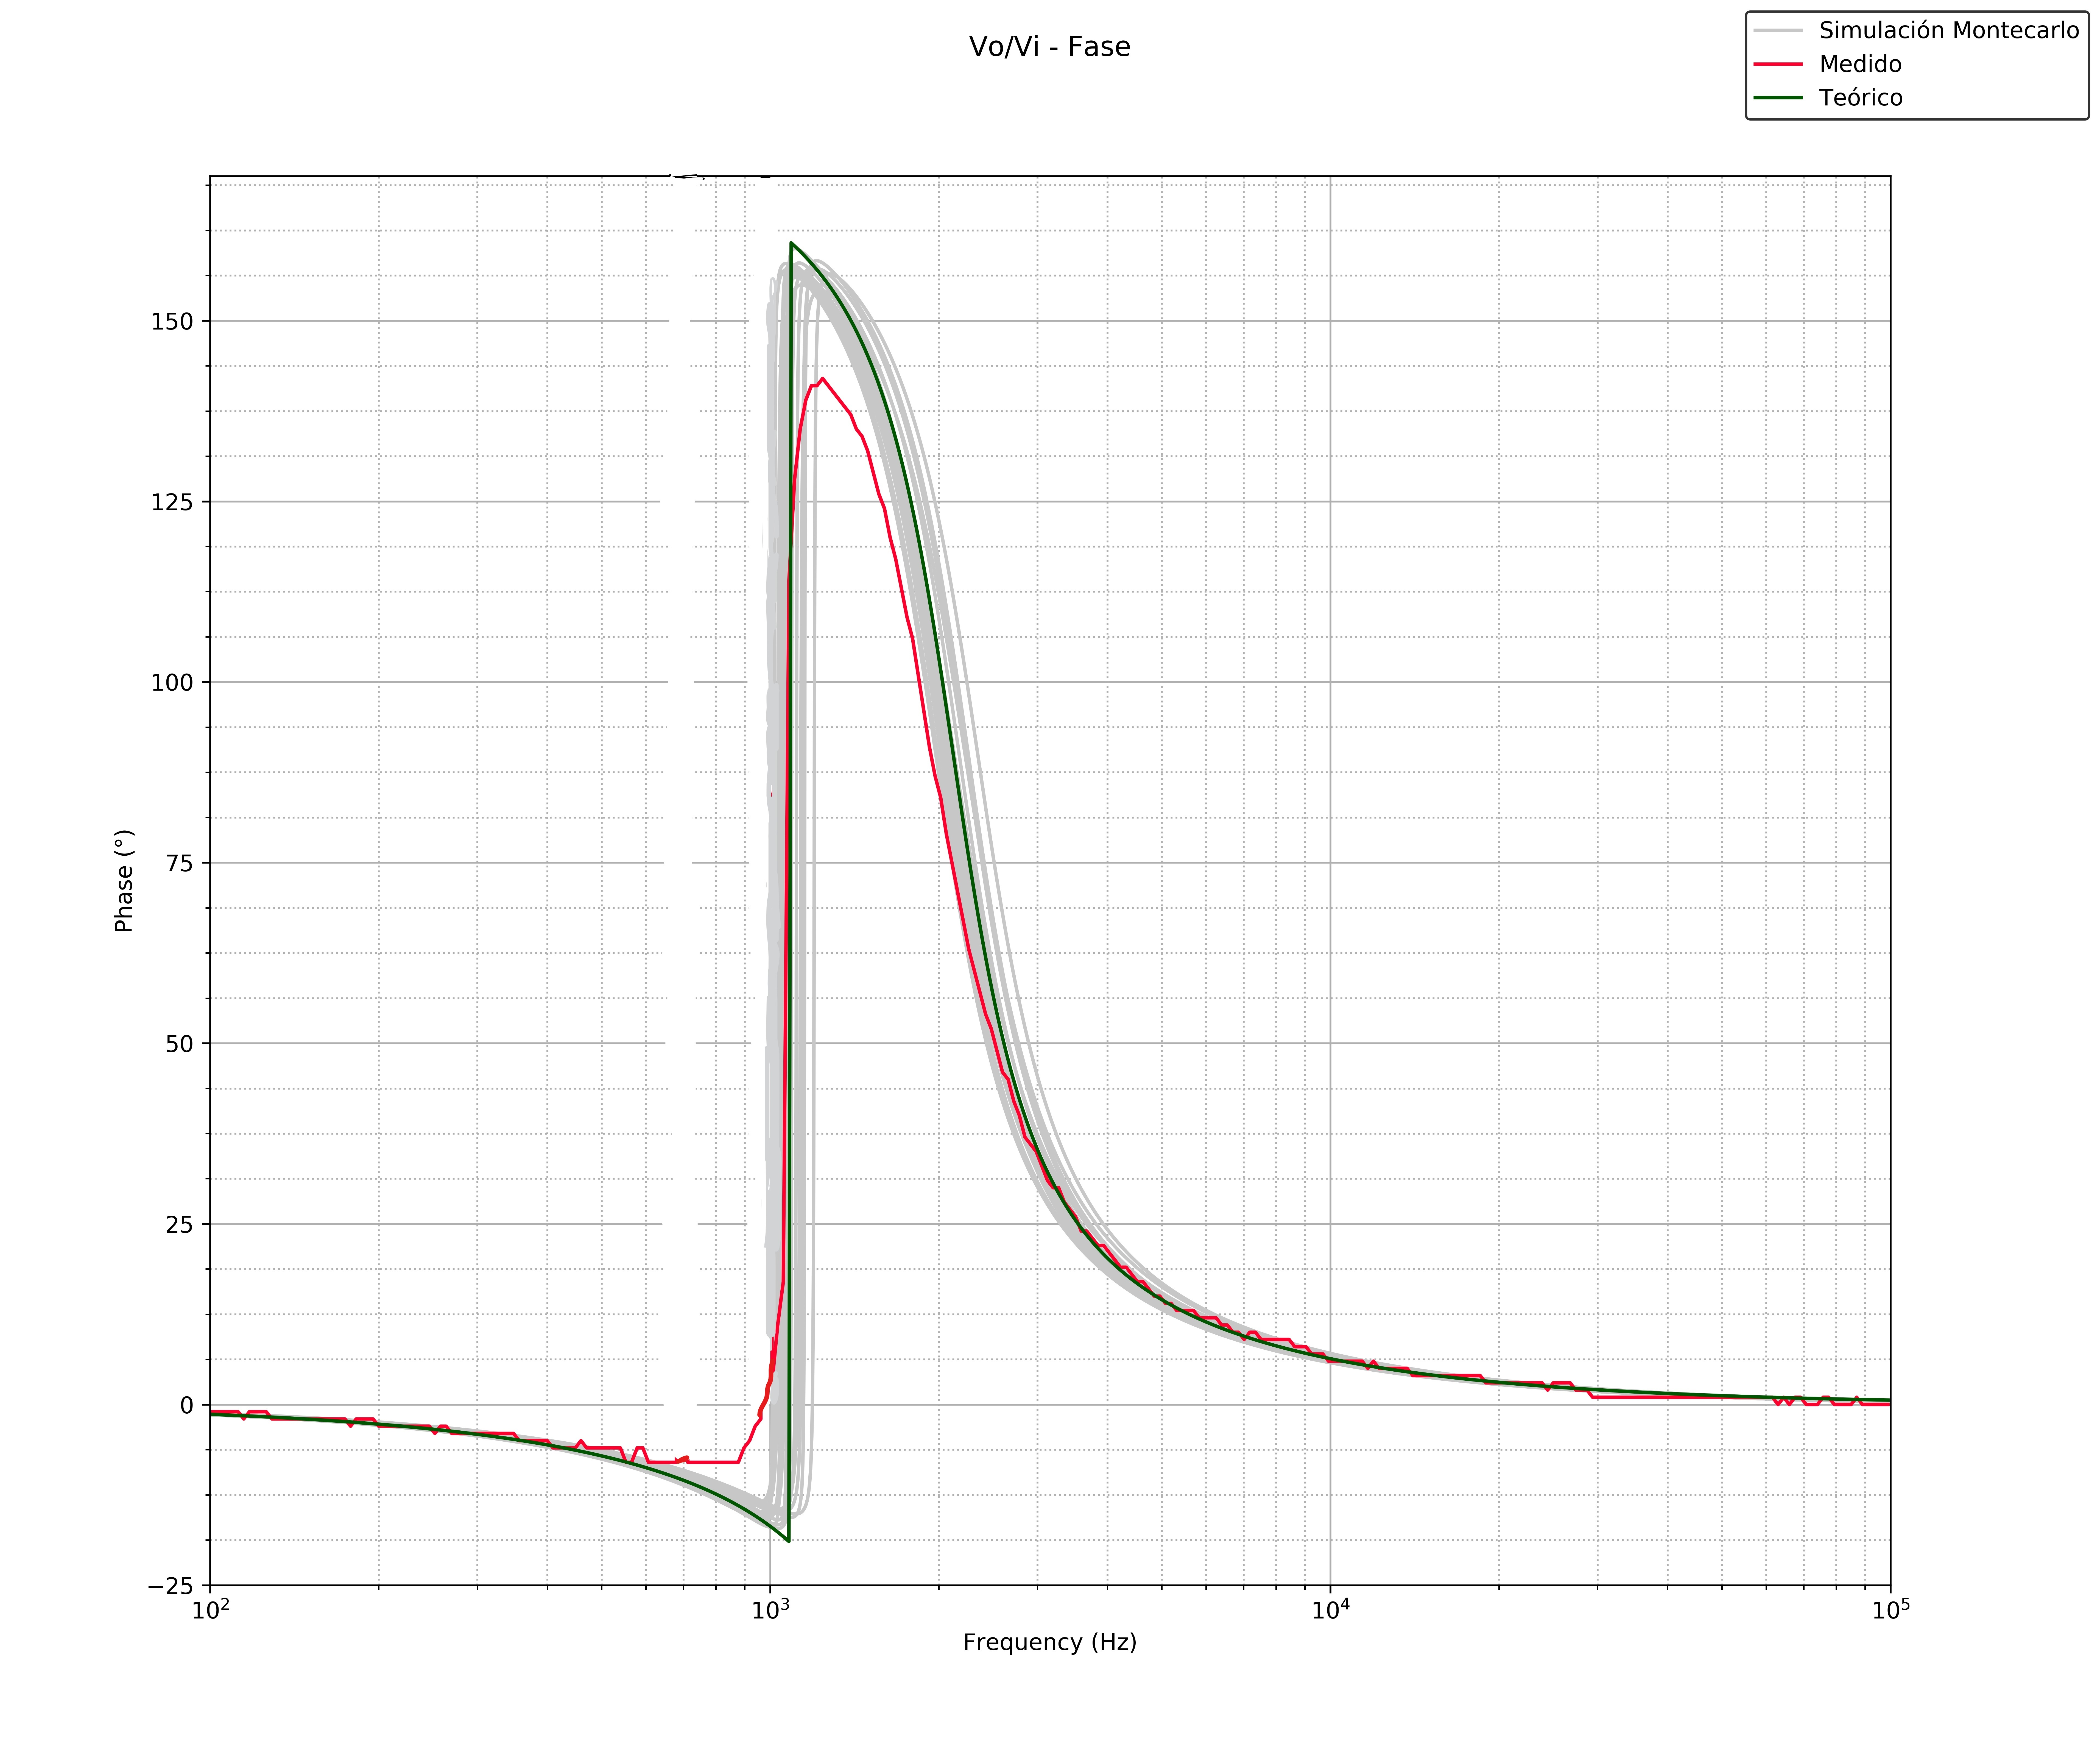
\includegraphics[width=10cm,height=10cm,keepaspectratio]{../EJ1/00GRAFICOS/vovifase.jpg}
	\caption{Fase de la transferencia del circuito.}
	\label{vovi_fase}
\end{figure}

El gr\'afico del m\'odulo de la funci\'on transferencia, figura \ref{vovi_mod}, permite ver que los Q de la medici\'on fueron menores que aquellos de los c\'alculos te\'oricos. Si bien el Q del polo presenta una peque\~na respecto a la especificada te\'oricamente en el dise\~no del circuito, el Q del cero presenta un cambio notable. Te\'oricamente el mismo deb\'a ser infinito, pero en la implementaci\'on eso no ocurre. Sin embargo, la atenuaci\'on no deja de ser considerable.


\subsection{ ''Notch Depth''}

Se llama $notch$  $depht$ a la profundidad del pico del filtro notch. Esta profundidad es la m\'axima atenuaci\'on que presentar\'a la se\~nal de entrada.

\paragraph*{C\'alculo anal\'itico:} Observando la funci\'on transferencia ideal del circuito, que se transcribe a continuaci\'on:

\begin{equation}
H(s) = \frac{2}{1+k^2} \cdot \frac{s^2 + \left( \frac{k}{RC}\right)^2}{s^2 + \frac{1}{RCQ} s + \left(\frac{1}{RC}\right)^2}
\label{vovi_simple2}
\end{equation}

Se puede decir que dado que el Q del cero es $\infty$, el pico del notch deber\'a tener una atenuaci\'on infinita. Esto es para el caso ideal, el cual no se cumple al momento de medir. Para ver anal\'iticamente lo que ocurre con el pico del notch, se evalu\'o $H(s=j2\pi f)$ para obtener la funci\'on transferencia en funci\'on de la frecuencia en Hz. Luego se tom\'o su m\'odulo y se busc\'o su m\'inimo, obteniendo para este una frecuencia de $1,082kHz$. A esta frecuencia deber\'ia estar te\'oricamente el pico del notch.

\paragraph*{Medici\'on:} Para medir la frecuencia y la atenuaci\'on del pico del notch, primero se intent\'o hacerlo con el bodeador. Al ir achicando el rango de frecuencias en la zona del pico y al exigirle al programa la obtenci\'on de m\'as puntos de medici\'on, se not\'o que la atenuaci\'on del pico iba variando, haciendose cada vez mayor. La atenuaci\'on m\'axima que se logr\'o obtener de esta forma fue de $\approx 30dB$. Este resultado se muestra en el gr\'afico \ref{pico}. En este gr\'afico se compara lo medido con lo te\'orico y con simulaci\'on Montecarlo, pero tambi\'en se contrasta con la simulaci\'on del valor exacto (ideal y deseado) de los componentes elegidos y teniendo en cuenta las puntas. Al estar analizando una zona de detalle, se compar\'o con la simulaci\'on reci\'en aclarada y no solo con el Montecarlo ya que el mismo presenta curvas muy exparsidas y pod\'ia ser relevante observar a qu\'e ser\'a mejor aproximarse y poder entender qu\'e tan lejos o cerca se logr\'o llegar de la frecuencia y de la atenuaci\'on del pico del notch.

\begin{figure}[H] %!ht
	\centering
	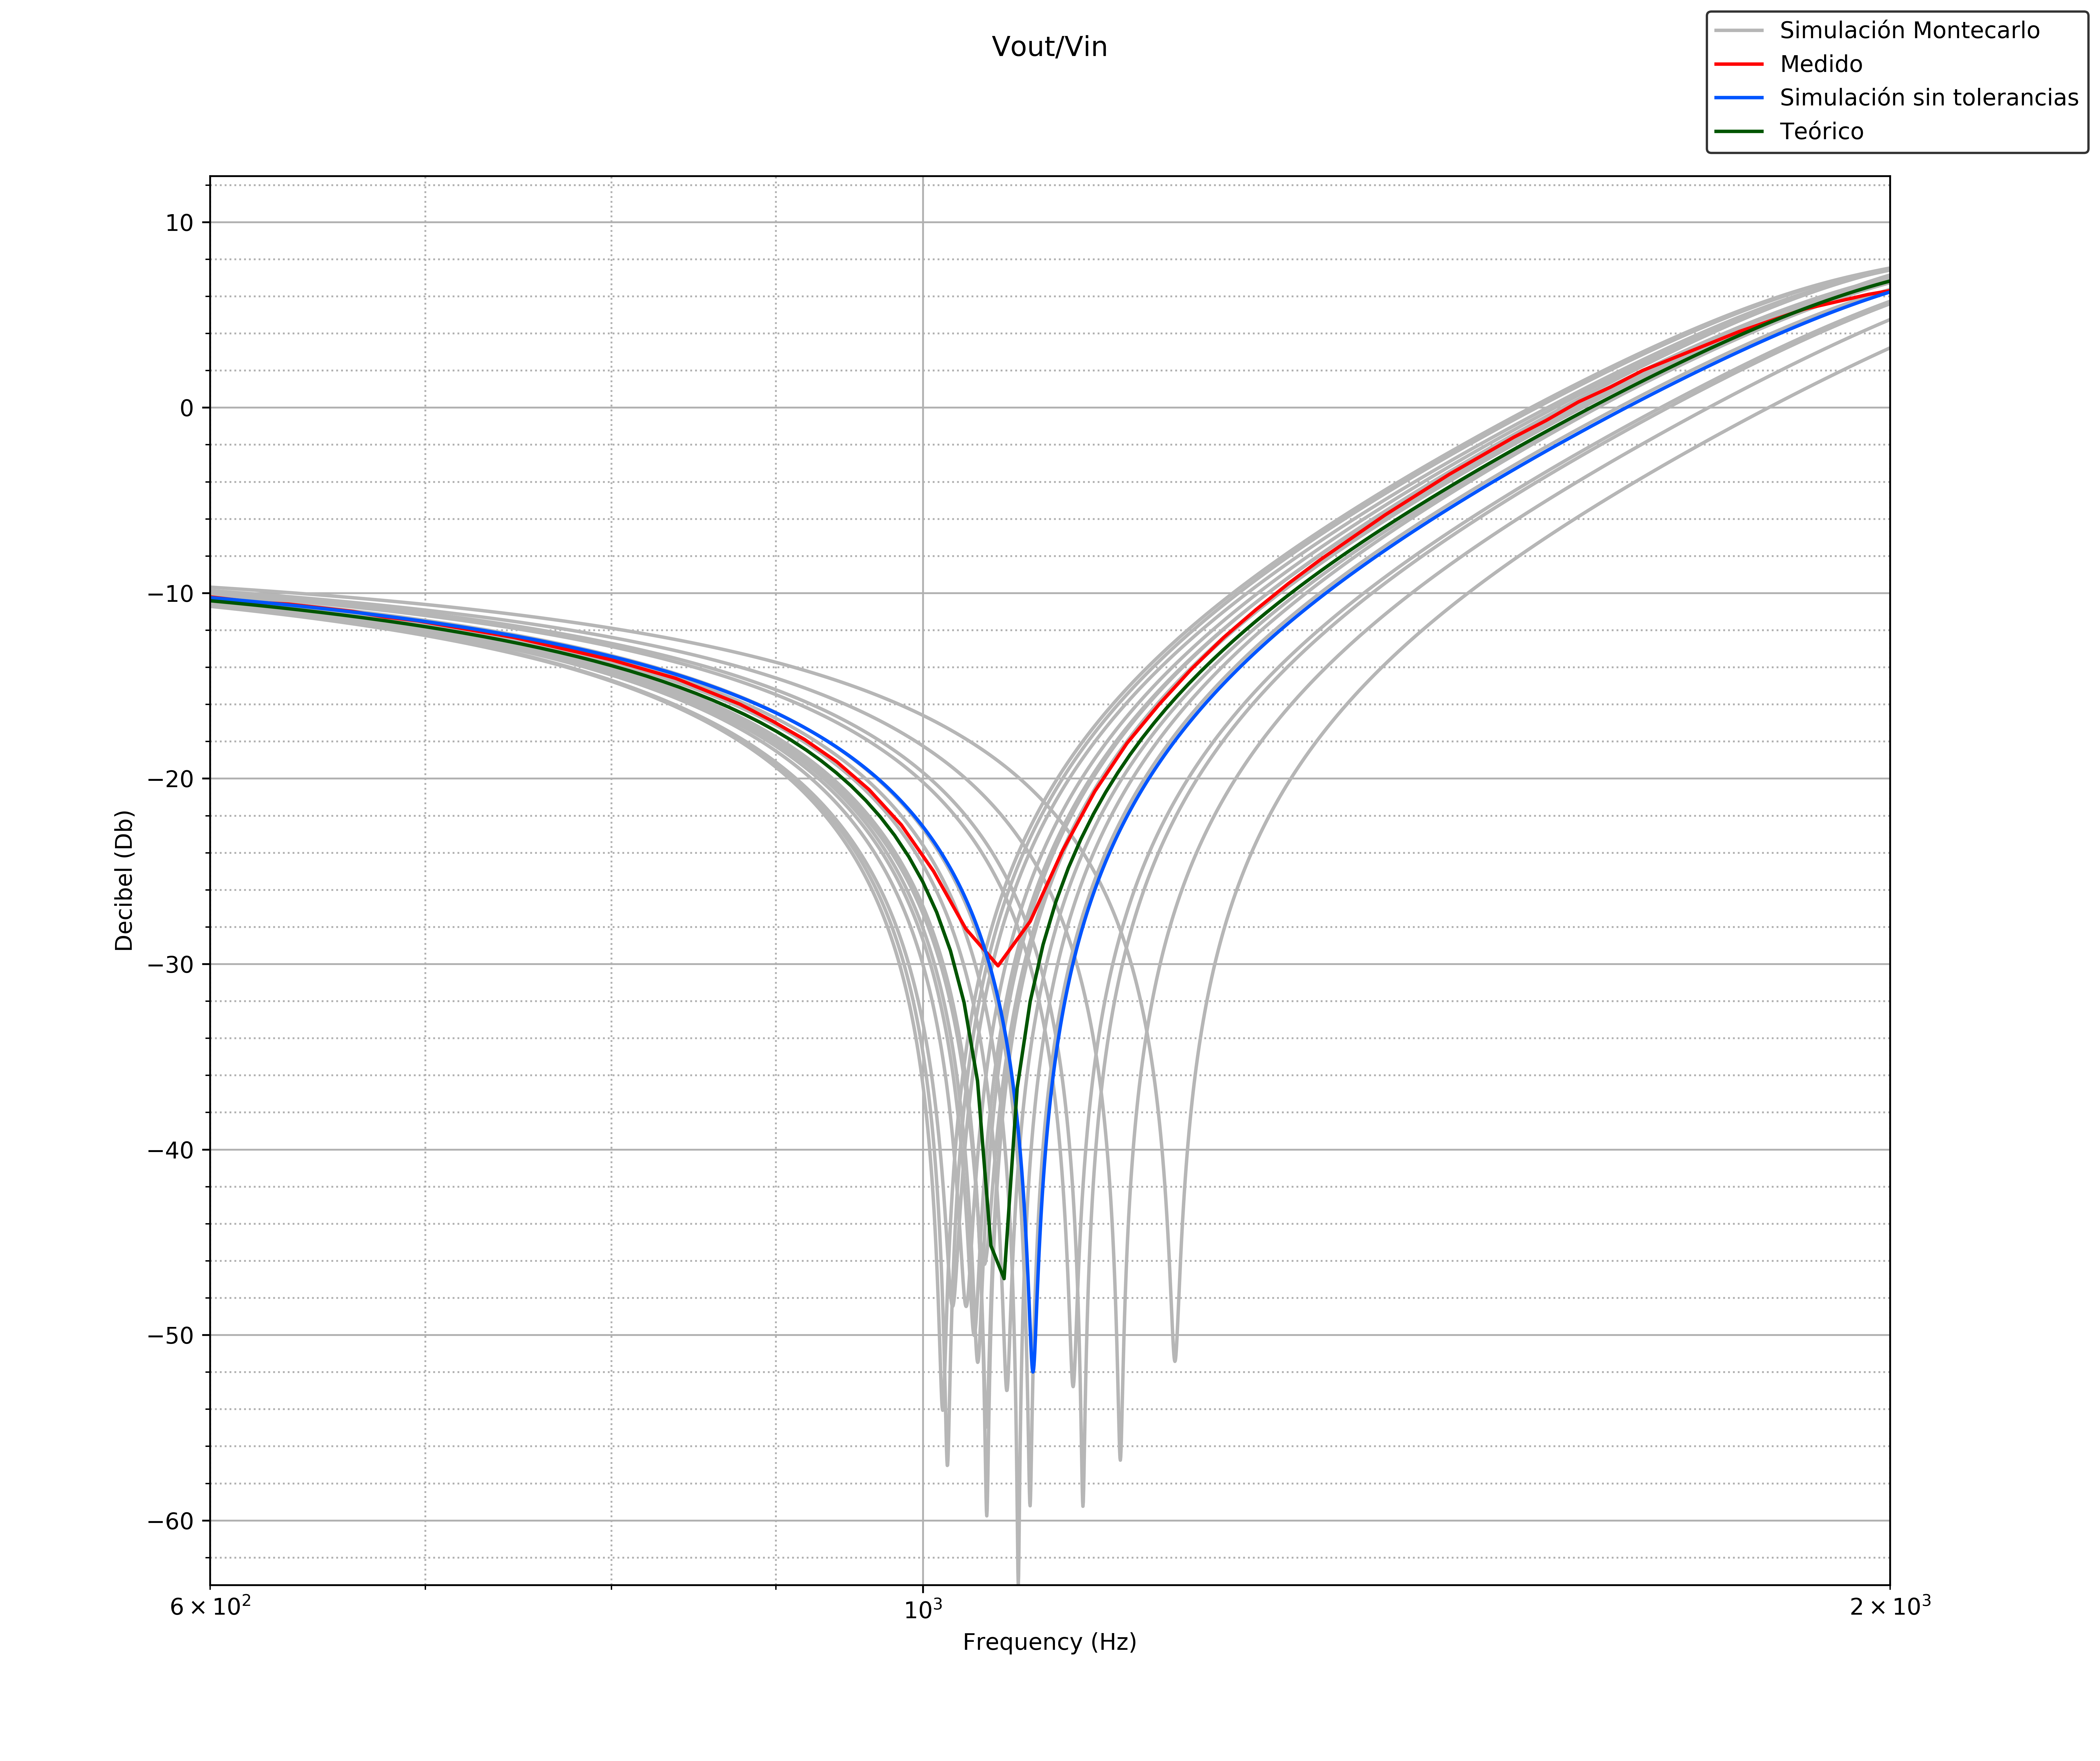
\includegraphics[width=10cm,height=10cm,keepaspectratio]{../EJ1/00GRAFICOS/pico.png}
	\caption{Detalle del pico del notch.}
	\label{pico}
\end{figure}

Al percatarse de que pod\'ian no ser suficientes los puntos tomados en la zona del pico, luego, empleando el osciloscopio manualmente, se busc\'o la frecuencia para la cual la salida es m\'inima, obteniendo $1,097kHz$. Para dicho punto se obtuvo una atenuaci\'on de $\approx35dB$, la cual es menor que la predicha con los c\'alculos te\'oricos al no tratarse de un filtro notch ideal, pero con una atenuaci\'on de $5dB$ m\'as que la previamente obtenida con el bodeador. Por lo tanto, se verific\'o que en el proceso de medici\'on de la funci\'on transferencia este pico tambi\'en se lo vio con menor atenuaci\'on debido al m\'etodo de medici\'on.


\subsection{Impedancia de entrada}
Para medir la impedancia de entrada del circuito en funci\'on de la frecuencia, 
deb\'iamos hacer el cociente $V_{in}/I_{in}$. Si bien se puede medir la tensi\'on 
de entrada al circuito de forma directa con el osciloscopio, 
no es tan sensillo obtener la corriente que entra al circuito, ya que el osciloscopio 
mide tensiones y no corrientes. Se busc\'o una resistencia $R_L$ cuyo valor comerical 
fuera lo m\'as parecido posible (igual o el primero mayor) al valor obtenido en 
el c\'alculo te\'rico para cada uno de los casos de resistencias. Se coloc\'o dicha 
resistencia en serie al generador, a la entrada del circuito. Luego se midi\'o la ca\'ida 
de tensi\'on sobre ella, ya que al dividirla por el valor de la $R_L$ colocada se obtendr\'ia 
la corriente de entrada al circuito $I_{in}$. El criterio de buscar una resistencia similar 
al valor calculado de $Z_{in}$ surge de que si se pusiese una resistencia muy chica, 
la diferencia entre las tensiones medidas sobre sus bornes ser\'ia muy chica 
(aumentando incertidumbre) y si se colocase una resistencia muy grande, 
la tensi\'on que caer\'ia ser\'ia mucho mayor a la que caer\'ia en el circuito, 
haciendo que la tensi\'on luego de la resistencia sea muy chica (se podr\'ia 
acercar al nivel de ruido) y que la diferencia de tensi\'on entre sus bornes tienda 
a la tensi\'on entregada por el generador. Por eso se consider\'o \'optimo que la 
resistencia tenga un valor similar al calculado de forma te\'orica y en caso de no 
conseguir el mismo valor, prefiri\'endose un valor mayor y no menor. 

En la expresi\'on \ref{zinn} se presenta la impedancia de entrada del circuito luego de haber reemplazado por los valores de los componentes:
\begin{equation}
Zin(s) =  (R_7 // C_6 // R_8)+(R_5//R_6)=\frac{21,94 \cdot 10^8 s + 8,55 \cdot 10^13}{53,22 \cdot 10^5 s + 7,846 \cdot 10^7}
\label{zinn}
\end{equation}


En los siguientes gr\'aficos se observa la impedancia de entrada medida y simulada con el m\'etodo de Montecarlo.
\begin{figure}[H] %!ht
	\centering
	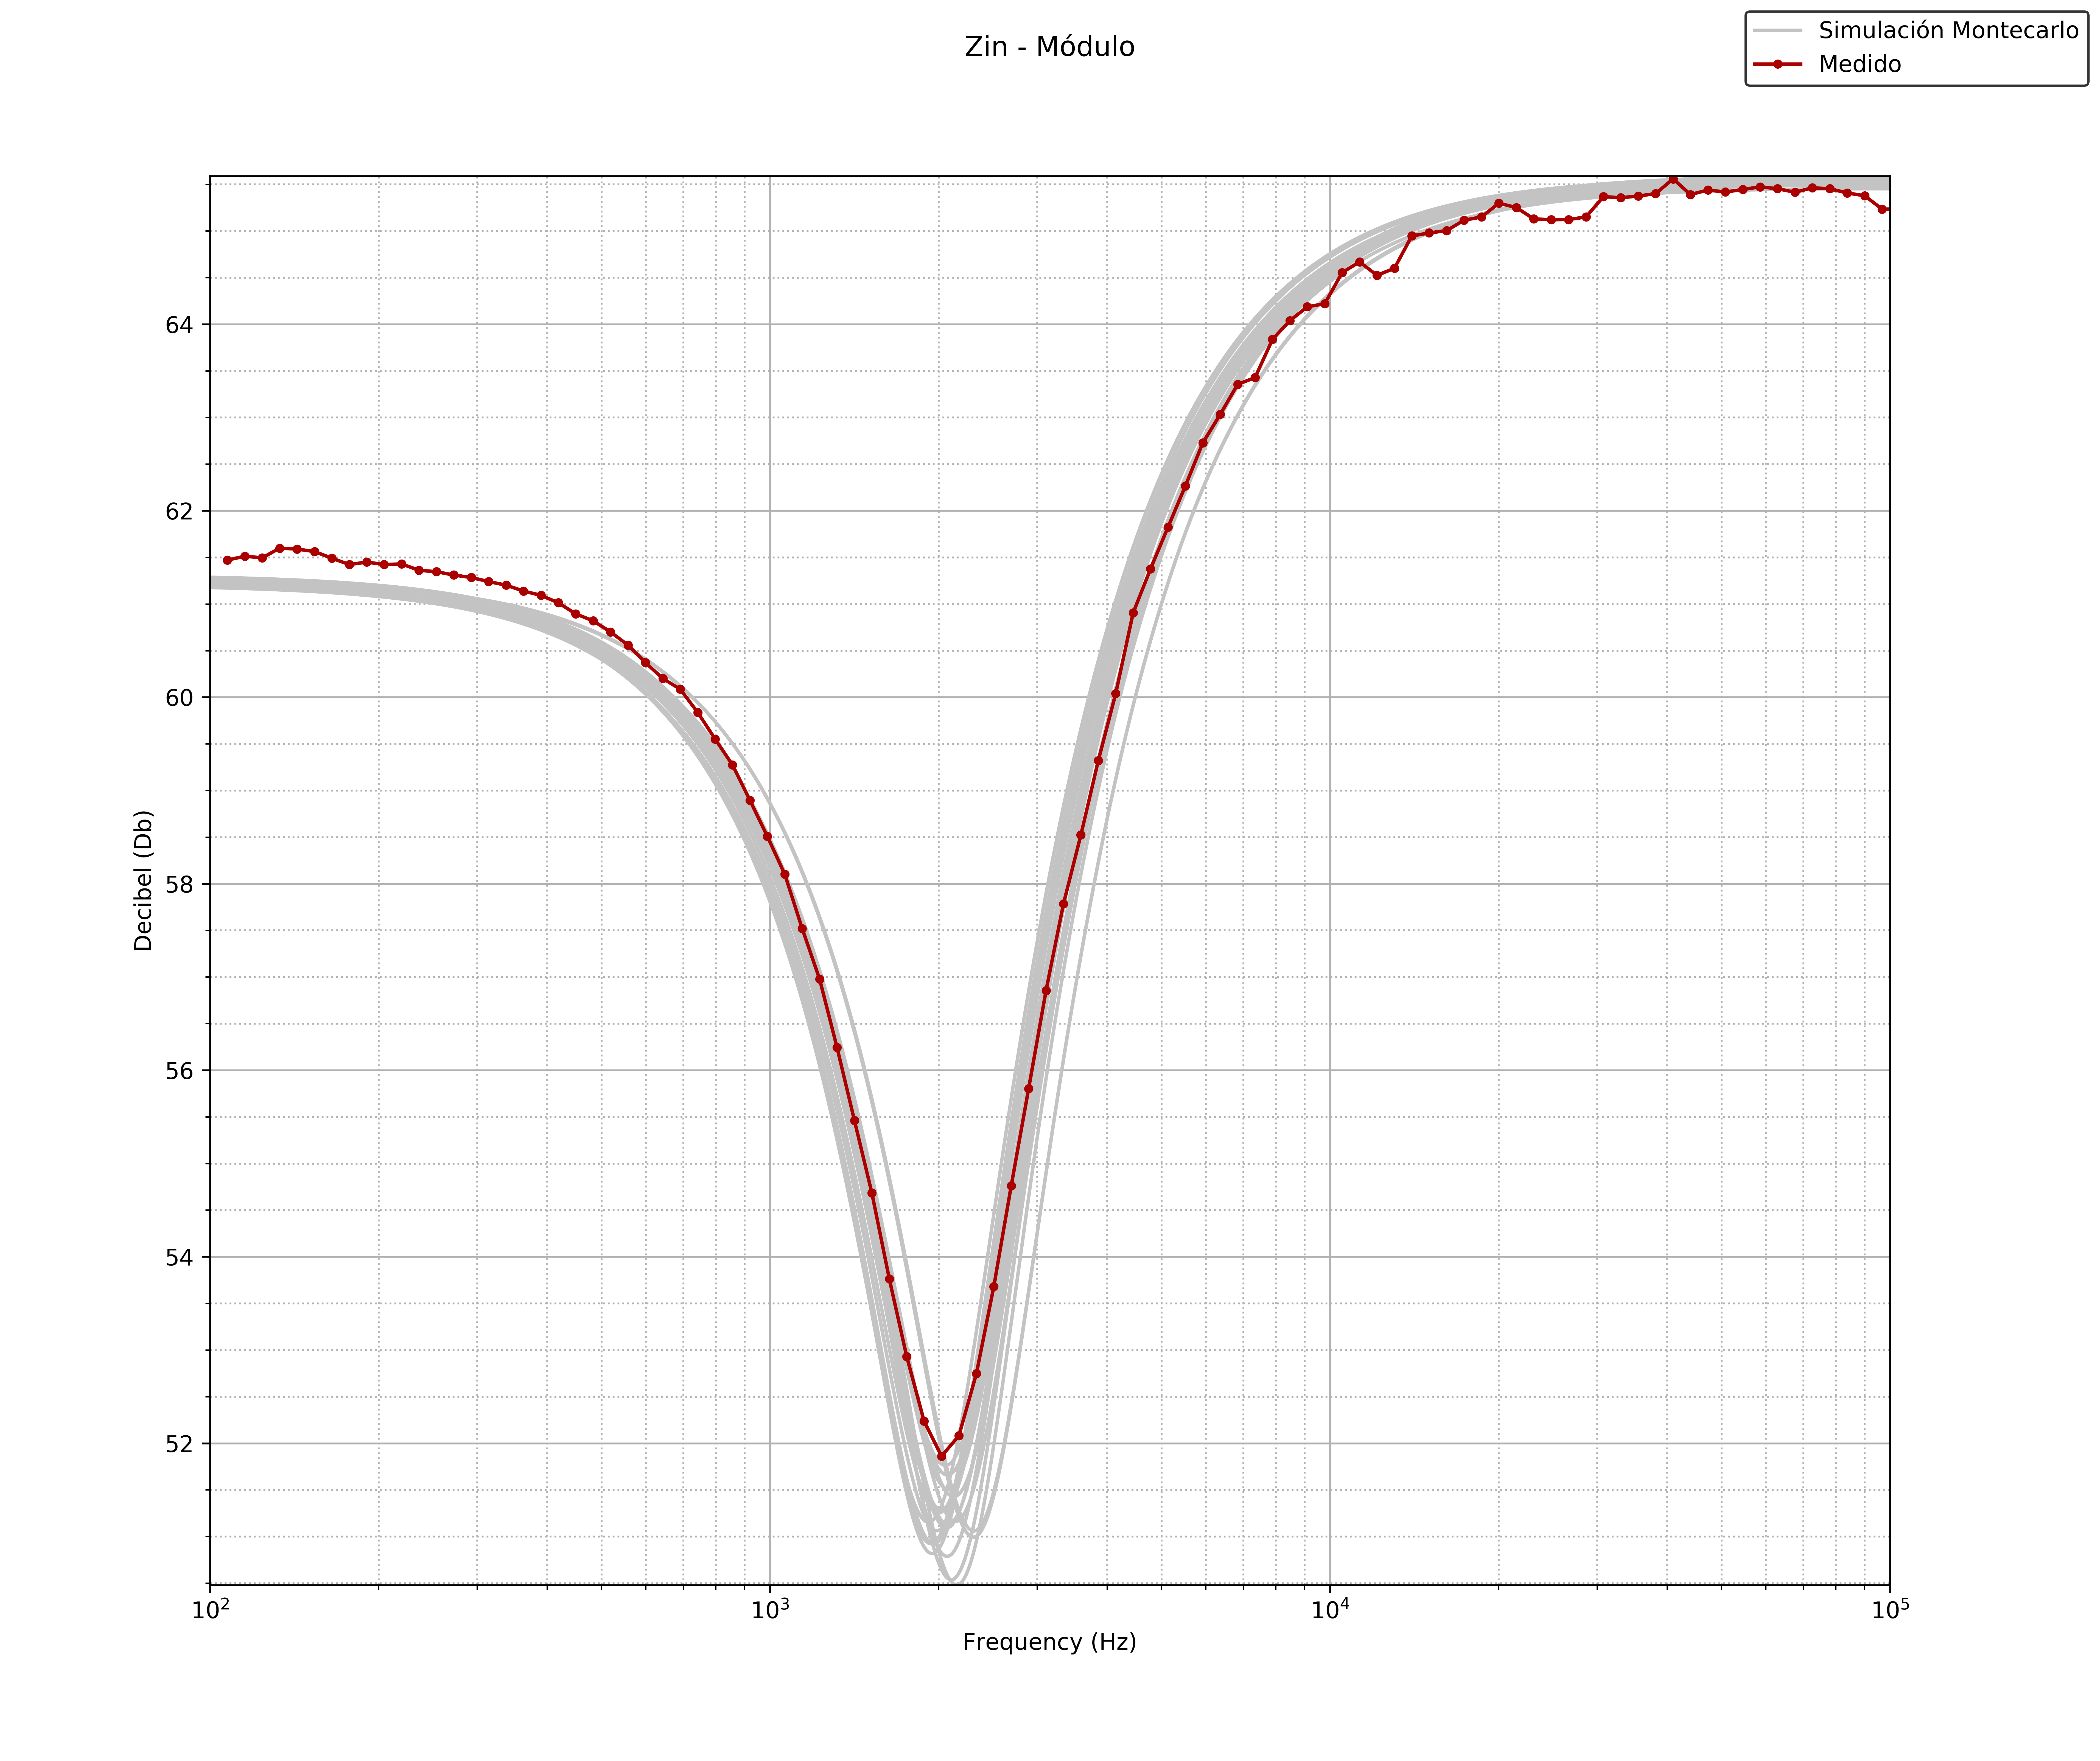
\includegraphics[width=10cm,height=10cm,keepaspectratio]{../EJ1/00GRAFICOS/zin_modulo_sinTeorico.png}
	\caption{Impedancia de entrada.}
	\label{zin_mod}
\end{figure}

\begin{figure}[H] %!ht
	\centering
	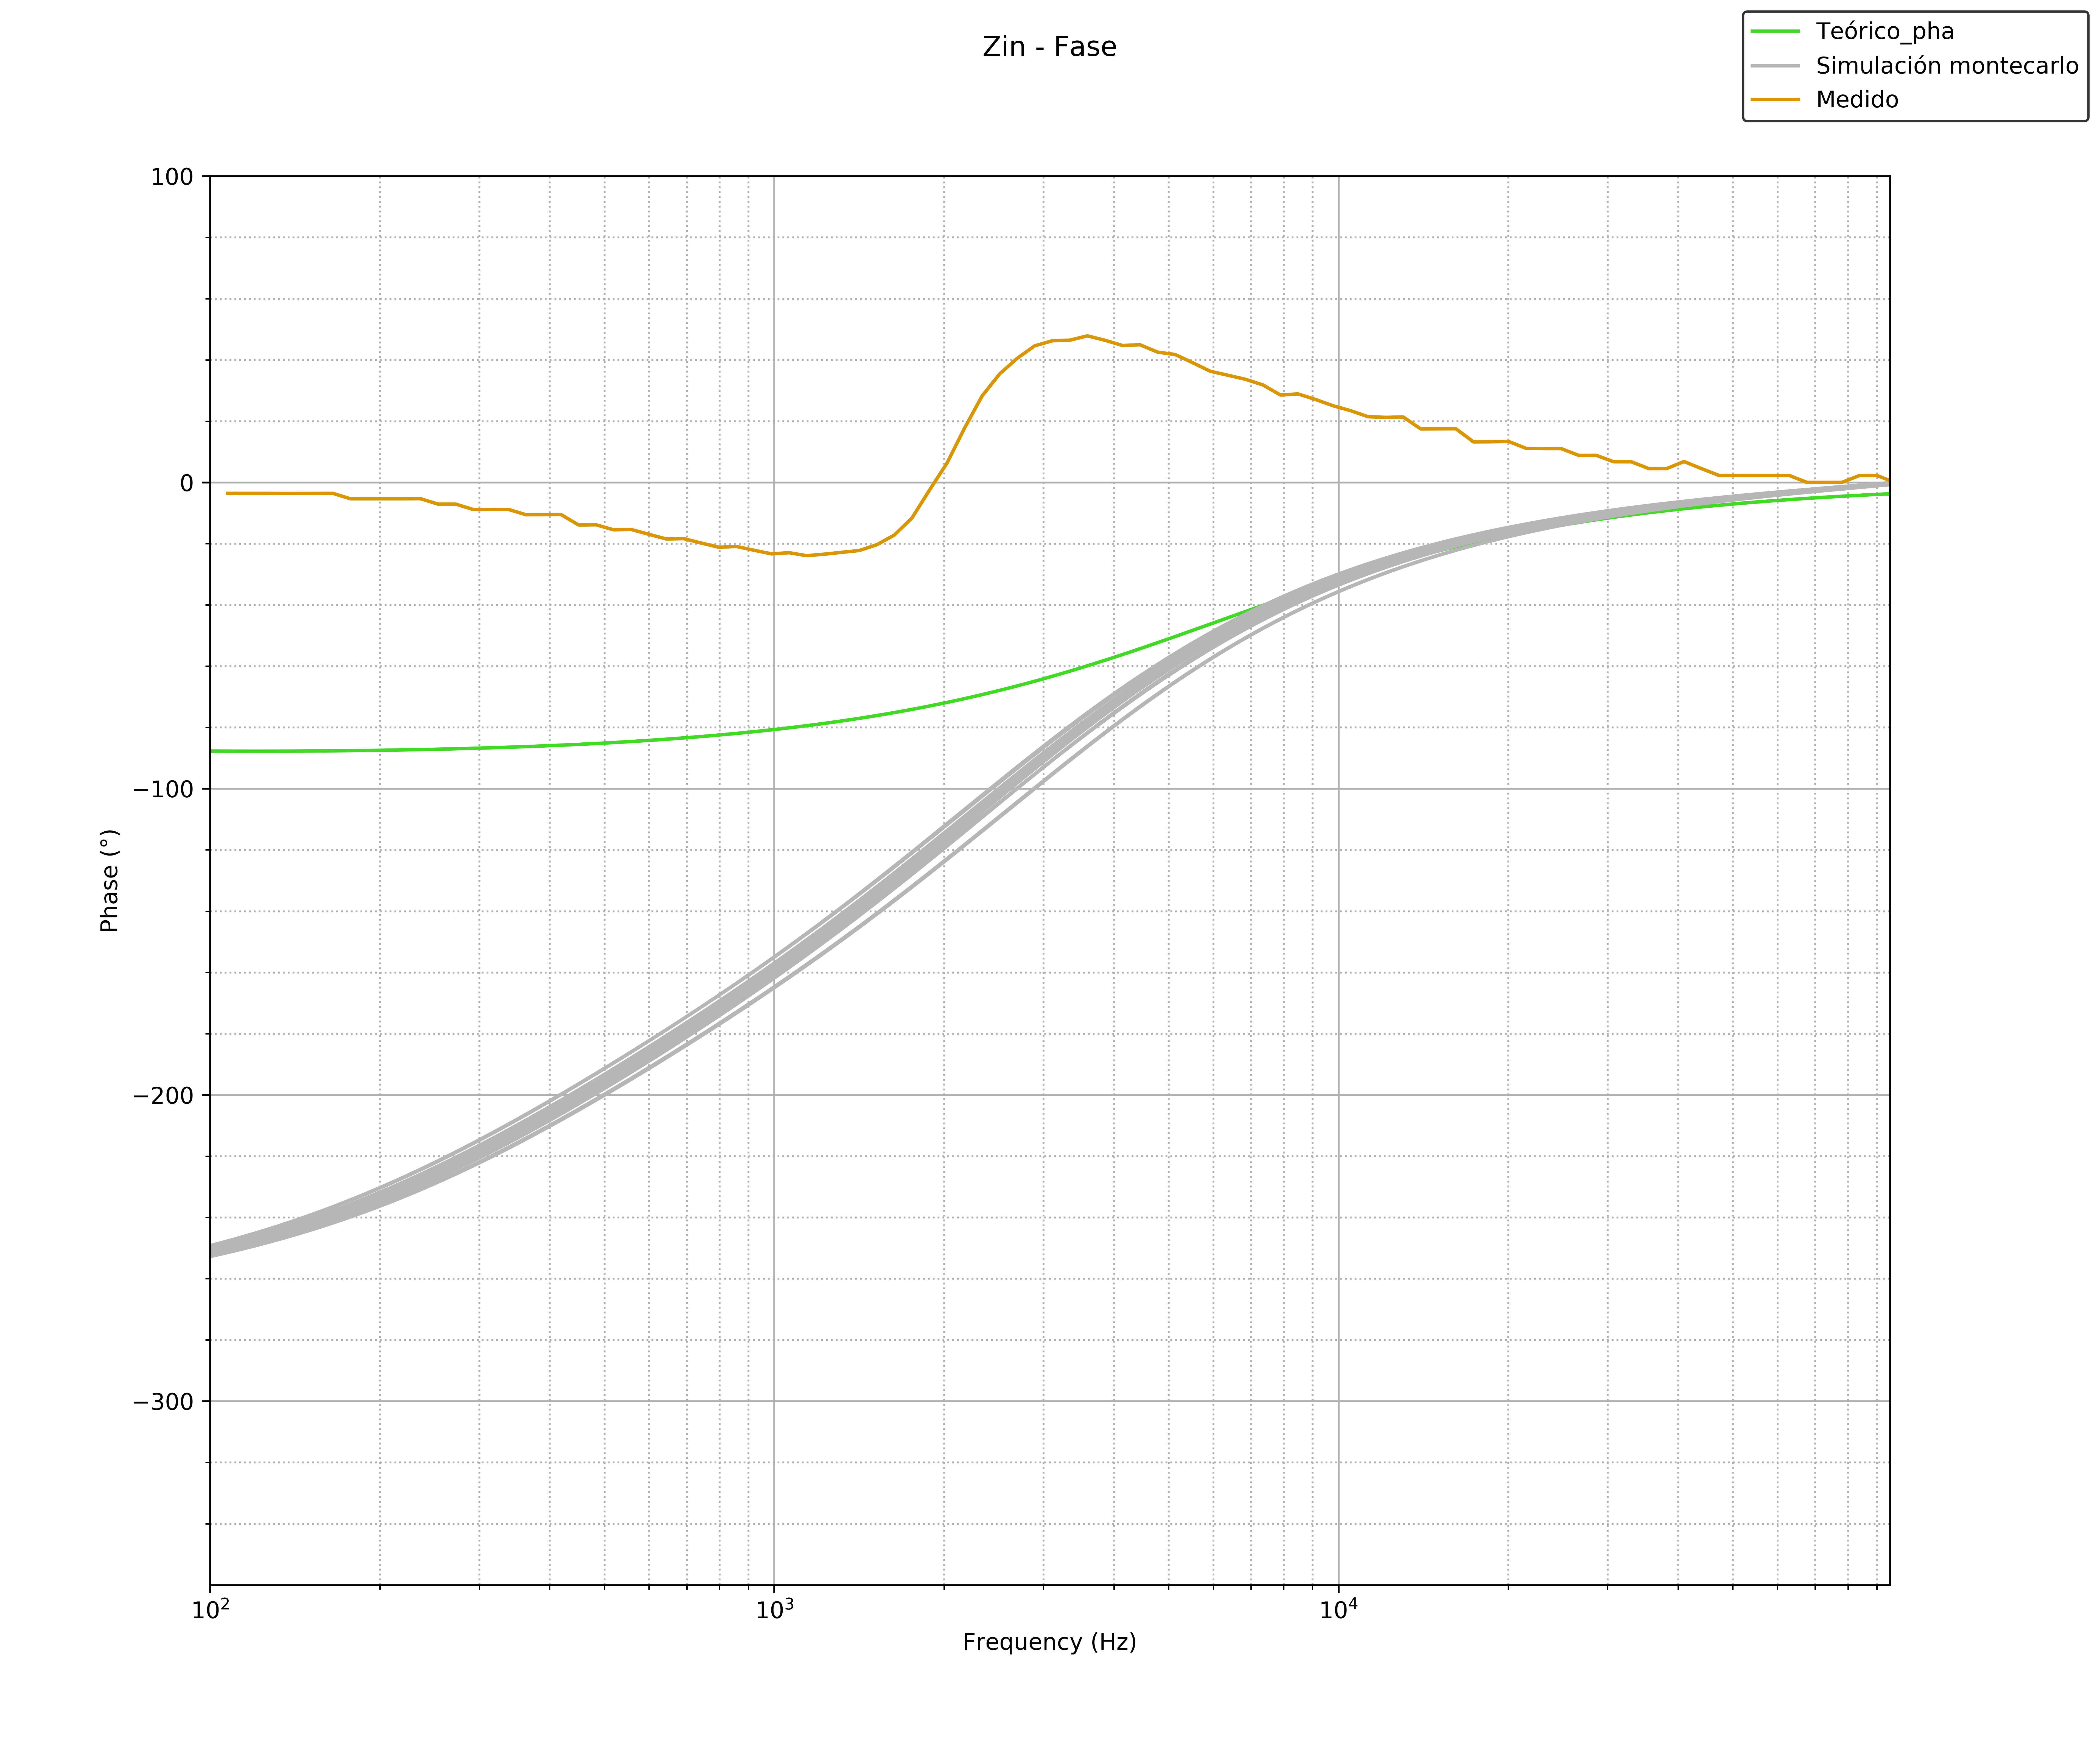
\includegraphics[width=10cm,height=10cm,keepaspectratio]{../EJ1/00GRAFICOS/zinn.png}
	\caption{Impedancia de entrada.}
	\label{zin_fase}
\end{figure}

Se considera que hay algo mal en la fase de la impedancia de entrada.

\subsection{Impedancia de salida}

En esta parte se detallar\'a el m\'etodo empleado para medir la impedancia de salida, pero se anticipa al lector que no se considera que el mismo haya funcionado como se esperaba. 

Al tener un circuito con componentes activos, desde un primer momento se descart\'o la opci\'on de medir la impedancia de salida pasivando la fuente de entrada y colocando una fuente a la salida para medirla como si esta fuera una impedancia de entrada vista desde la nueva fuente. Por esta raz\'on se prosigui\'o de la siguiente forma.

\begin{figure}[H] %!ht
	\centering
	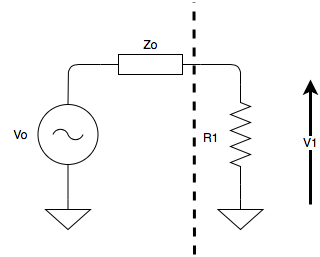
\includegraphics[width=8cm,height=8cm,keepaspectratio]{../EJ1/00GRAFICOS/zout.png}
	\caption{Impedancia de entrada.}
	\label{zout}
\end{figure}

El circuito de la figura \ref{zout} representa a nuestro circuito en el momento de medir. Se considera como circuito equivalente para el high pass notch a una fuente de tensi\'on $Vo$ en serie con la $Zo$ que se quiere medir. Primero se conecta a la salida del circuito una resistencia R1 y se mide la tensi\'on $V1$ sobre sus bornes. Luego se hace lo mismo con una resistencia R2, y se mide la tensi\'on sobre sus bornes, $V2$. Por divisor resistivo de tensi\'on:

\begin{equation}
\begin{cases}
V_1 = \frac{Vo R_1}{Zo + R_1}\\
V_2 = \frac{Vo R_2}{Zo + R_2}
\end{cases}
\label{v1v2}
\end{equation}

Considerando la misma $Vo$ para ambos casos, se dividen ambas expresiones de forma que se cancele dicha tensi\'on y se obtenga:

\begin{equation}
\frac{V_1}{V_2} = \frac{R_1}{Zo + R_1 } \cdot \frac{Zo + R_2}{R_2}
\end{equation}

Luego llamando $K = \frac{V_1}{V_2}\cdot \frac{R_2}{R_1} = \frac{Zo + R_2}{Zo + R_1}$, se obtiene:

\begin{equation}
\begin{cases}
Zo = \frac{R_2 - R_1 \cdot K}{K - 1}\\
K=\frac{V_1 R_2}{V_2 R_1}
\end{cases}
\label{zo}
\end{equation}

Para este m\'etodo, las resistencias empleadas a la salida deb\'ian ser, en nuestro caso, del orden de los $k\Omega$, para evitar que se rompiera la realimentaci\'on del opamp de salida, debido a la corriente. Se usaron resistencias de $33k\Omega$, $2k7\Omega$ y $10k\Omega$ con la finalidad de chequear el valor luego obtenido de la Zo a partir de m\'as de un par de resistencias, para disminuir la posibilidad de error.
Previamente se simularon las tensiones de salida con las mismas resistencias y considerando las puntas del osciloscopio y se observ\'o que daban igual. Esto implicar\'ia que al momento de medir no podr\'ia haber mucha diferencia de tensi\'on a la salida y dificultar\'ia el m\'etodo. Y as\'i fue. Se obtuvo una diferencia de tensi\'on de salida entre los distintos casos del orden de los $mV$, de forma que para calcular la Zo esa diferencia de tensi\'on estar\'ia en el nivel del piso de ruido. Realizar operaciones matem\'aticas sobre esta diferencia de tensi\'on tan chica, no ser\'ia un m\'etodo confiable.

\begin{figure}[H] %!ht
	\centering
	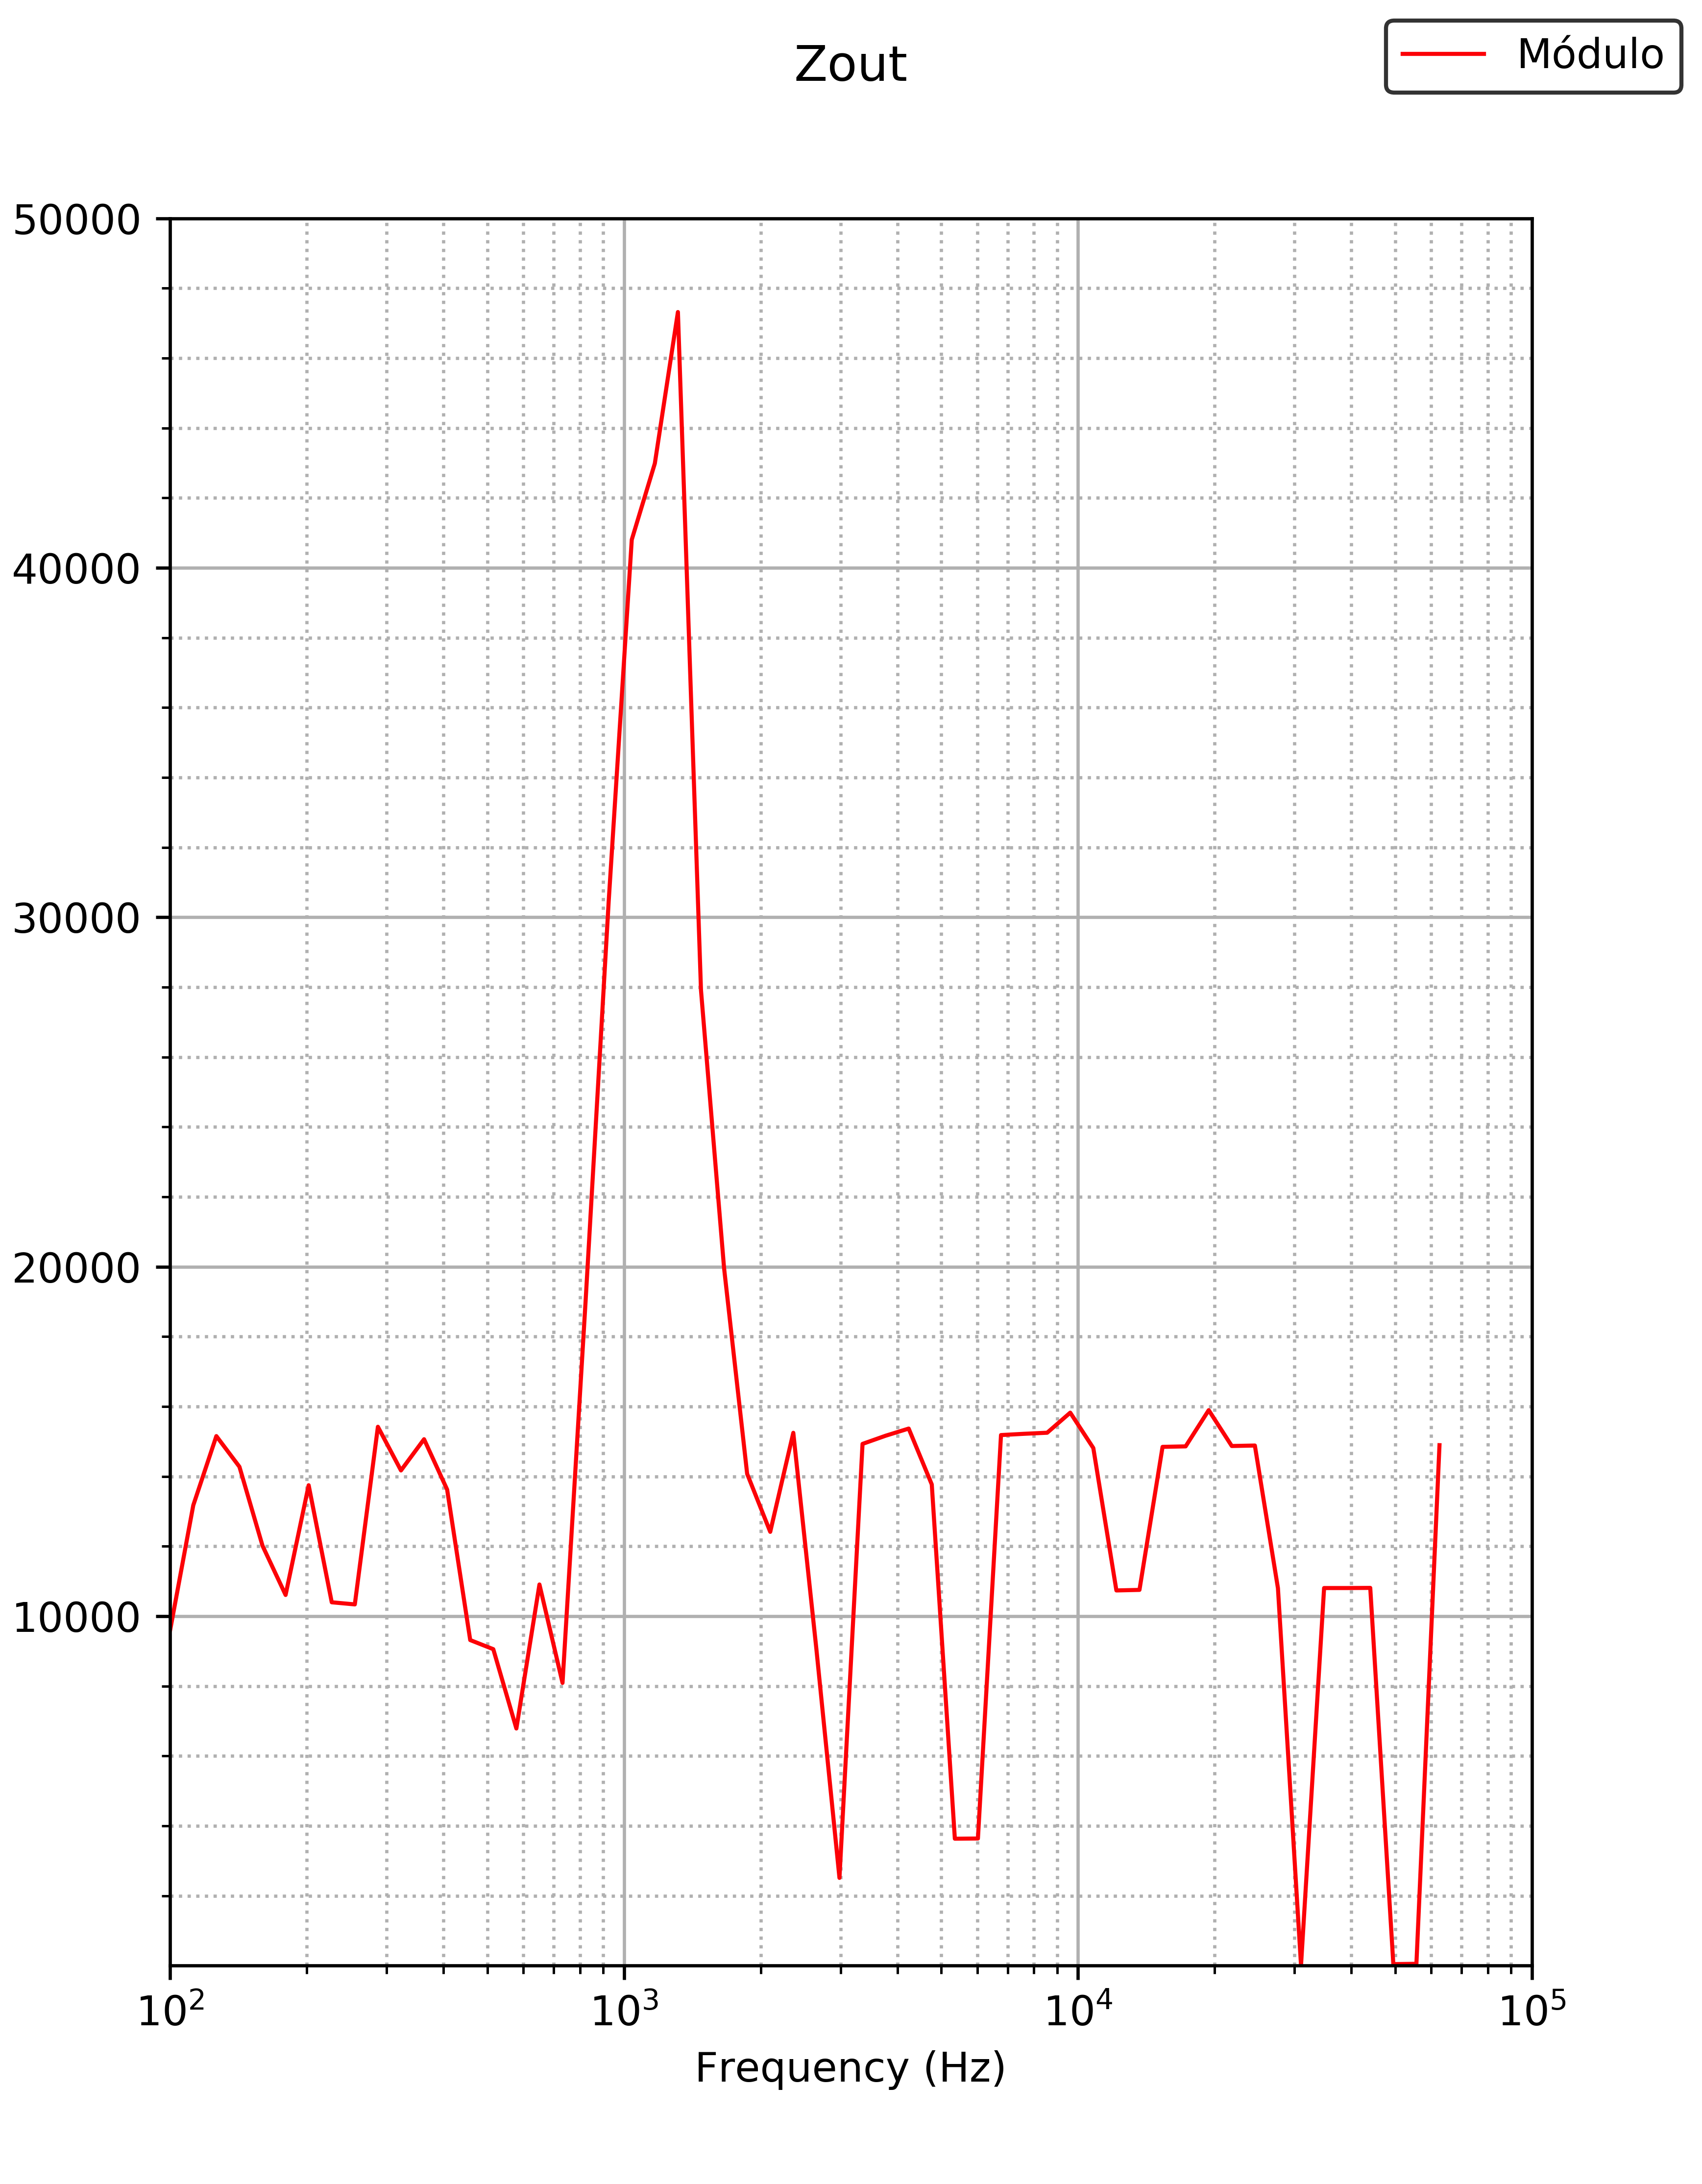
\includegraphics[width=10cm,height=10cm,keepaspectratio]{../EJ1/00GRAFICOS/zom.png}
	\caption{"Impedancia de salida" medida.}
	\label{zom}
\end{figure}

Algo interesante que se observa en el gr\'afico \ref{zom} es que hay un pico en su amplitud en la zona de frecuencias donde se encuentra el pico del filtro Notch. Sin embargo, no podemos afirmar que est\'e bien o mal lo obtenido. El gr\'afico fue logrado mediante c\'alculos con n\'umeros complejos para poder obtener Zo, pero las simulaciones, al haber sido tambi\'en sobre las tensiones medidas, requerir\'ian pasar por los mismos c\'alculos, lo cual impide que de forma r\'apida se sepa si est\'a bien lo obtenido (m\'as all\'a de la limitaci'on previamente mencionada sobre la gran probabilidad de tener error en el resultado al tener una diferencia de tensi\'on en el orden del piso de ruido).



\subsection{Limitación de tensi\'on de entrada}

La tensión de entrada máxima del circuito está limitada principalmente por el slew rate y la saturaci\'on. 

\subsubsection*{Influenccia del slew rate en $V_{in_{max}}$}

Partiendo de:
\begin{equation}
\begin{cases}
SR = m\'ax\bigg\{\frac{ dV_{out}}{dt}\bigg\} \\
V_{in} (f, t) = V_{in_{max}} \cdot sin(2\pi f t) \\
V_{out} (f, t) = \rvert H(f)\rvert \cdot V_{in_{max}} \cdot sin(2 \pi f t)
\end{cases}
\label{srecs}
\end{equation}

Siendo $SR$ el slew rate, $V_{in}$ y $V_{out}$ las se\~nales de entrada y de salida respectivamente y $\rvert H(f)\rvert = V_{out}/V_{in}$ la ganancia del circuito.


\begin{equation}
\frac{dV_{out}}{dt} = \rvert H(f)\rvert V_{in_{max}} 2 \pi f cos(2 \pi f t)
\label{deriv}
\end{equation}

Maximizando la ecuaci\'on \ref{deriv} se obtiene que:

\begin{equation}
SR = m\'ax\bigg\{\frac{dV_{out}}{dt}\bigg\} = \rvert H(f)\rvert 2 \pi f V_{in_{max}} 
\label{max}
\end{equation}

Despejando de la ecuaci\'on \ref{max}:

\begin{equation}
V_{in_{max}}  = \frac{SR}{\rvert H(f)\rvert 2\pi f}
\label{vinmax}
\end{equation}

El valor de SR, para el c\'alculo te\'orico, fue sacado de hojas de datos del amplificador operacional LM833 de Texas Instrument\footnote{Hoja de datos del operacional LM833: https://html.alldatasheet.com/html-pdf/784648/TI1/LM833/52/1/LM833.html}. 
Se encontr\'o que $SR = 7 \frac{V}{\mu s}$. Reemplazando con este valor en la expresi\'on \ref{vin_max}, se obtiene que la tensi\'on de entrada m\'axima limitada por el slew rate es:

\begin{equation}
V_{in_{max}}  = \frac{\left(17,36 \cdot 10^8 f^{4} - 1.37 \cdot 10^{16} f^{2} + 3.52 \cdot 10^{22}\right)}{f \sqrt{61,19 \cdot 10^5 f^{8} - 62,49 \cdot 10^{12} f^{6} + 2.45 \cdot 10^{20} f^{4} - 3.57 \cdot 10^{26} f^{2} + 1.70 \cdot 10^{32}}}		
\label{vin_max}
\end{equation}


\begin{figure}[H] %!ht
	\centering
	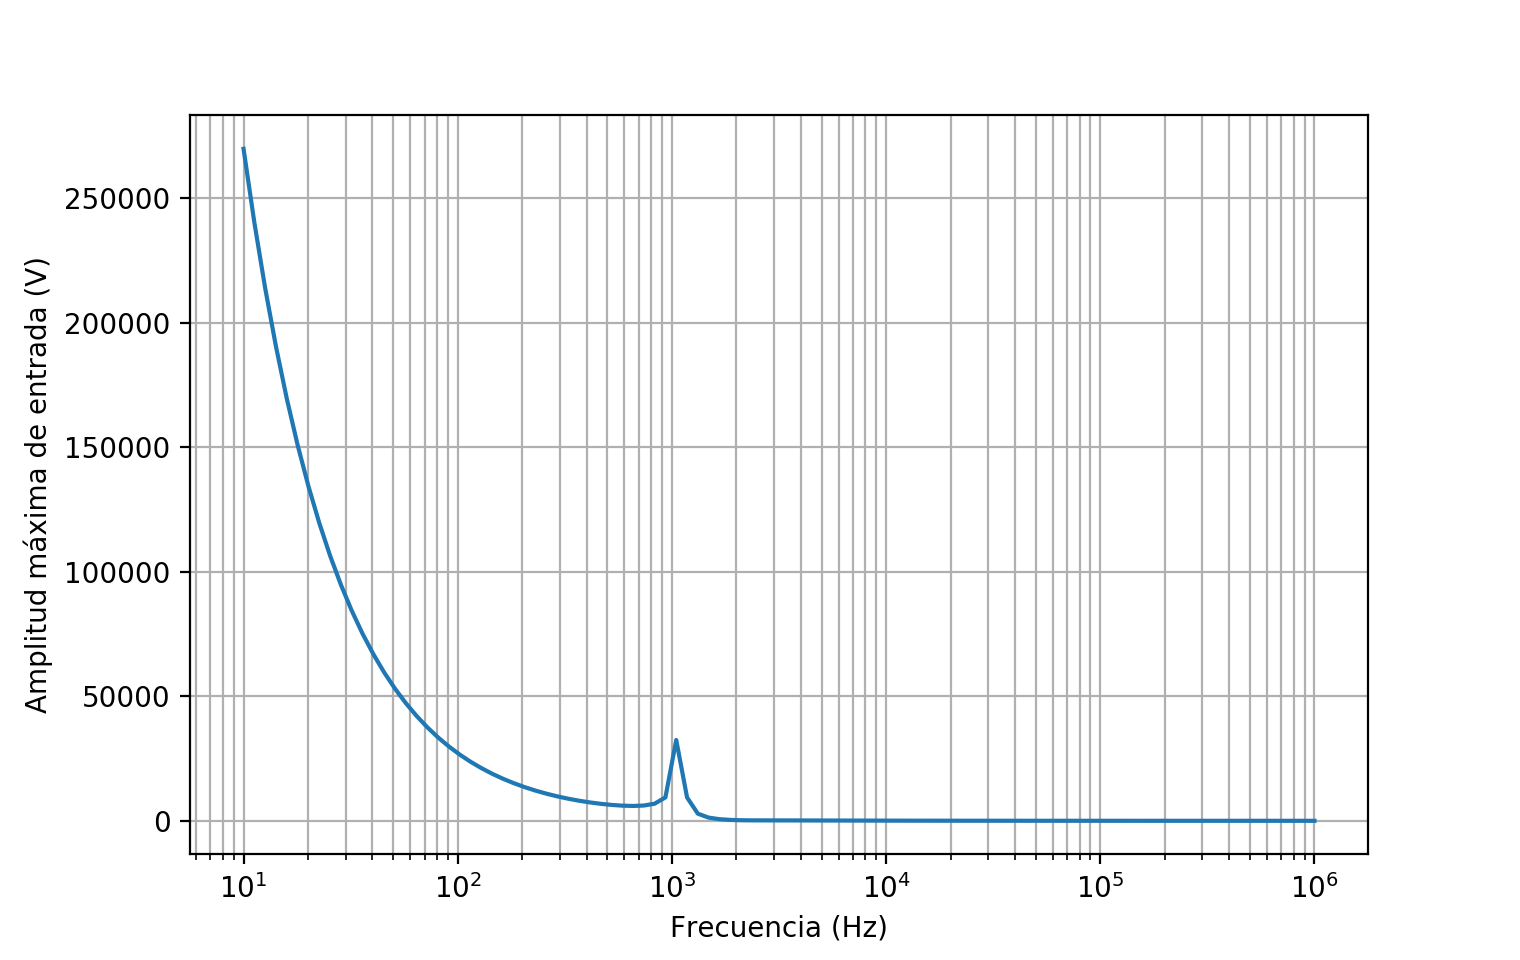
\includegraphics[width=10cm,height=10cm,keepaspectratio]{../EJ1/00GRAFICOS/vinmaxsr.png}
	\caption{Tensi\'on de entrada m\'axima limitada por slew rate.}
	\label{vinmaxsr}
\end{figure}

\subsubsection*{Influenccia de la saturaci\'on en $V_{in_{max}}$}
La tensi\'on pico a pico m\'axima de salida del amplificador operacional es llamada 
tensi\'on de saturasi\'on $V_{sat}$. Te\'oricamente, este valor es igual a $V_{CC}$. Dado que $V_{out} = \rvert H(s) \rvert V_{in}$:

\begin{equation}
V_{in_{max}} = \frac{V_{out_{max}}}{\rvert H(s) \rvert} = \frac{V_{sat}}{\rvert H(s) \rvert} = \frac{V_{CC}}{\rvert H(s) \rvert}
\end{equation}

Dado que en nuestro caso usamos $V_{CC} = \pm15V$, la expresi\'on que se obtiene es:

\begin{equation}
V_{in_{max}} = \frac{15V}{\rvert H(s) \rvert} 
\end{equation}


\begin{figure}[H] %!ht
	\centering
	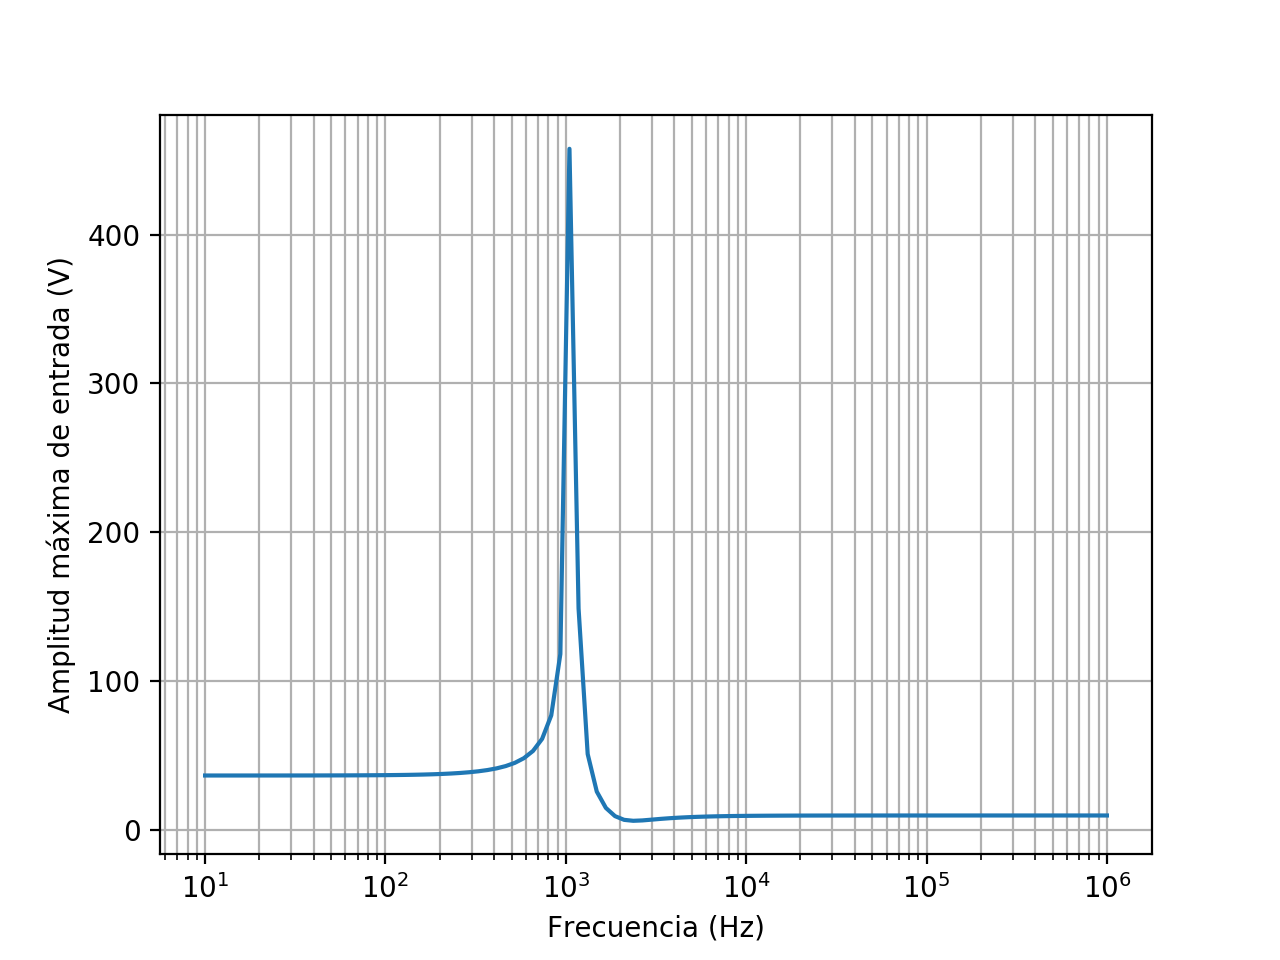
\includegraphics[width=10cm,height=10cm,keepaspectratio]{../EJ1/00GRAFICOS/vinmaxsat.png}
	\caption{Tensi\'on m\'axima de entrada limitada por saturaci\'on.}
	\label{vinmaxsat}
\end{figure}

\subsubsection*{Combinaci\'on del efecto de slew rate y saturaci\'on sobre la tensi\'on m\'axima de entrada}


\begin{figure}[H] %!ht
	\centering
	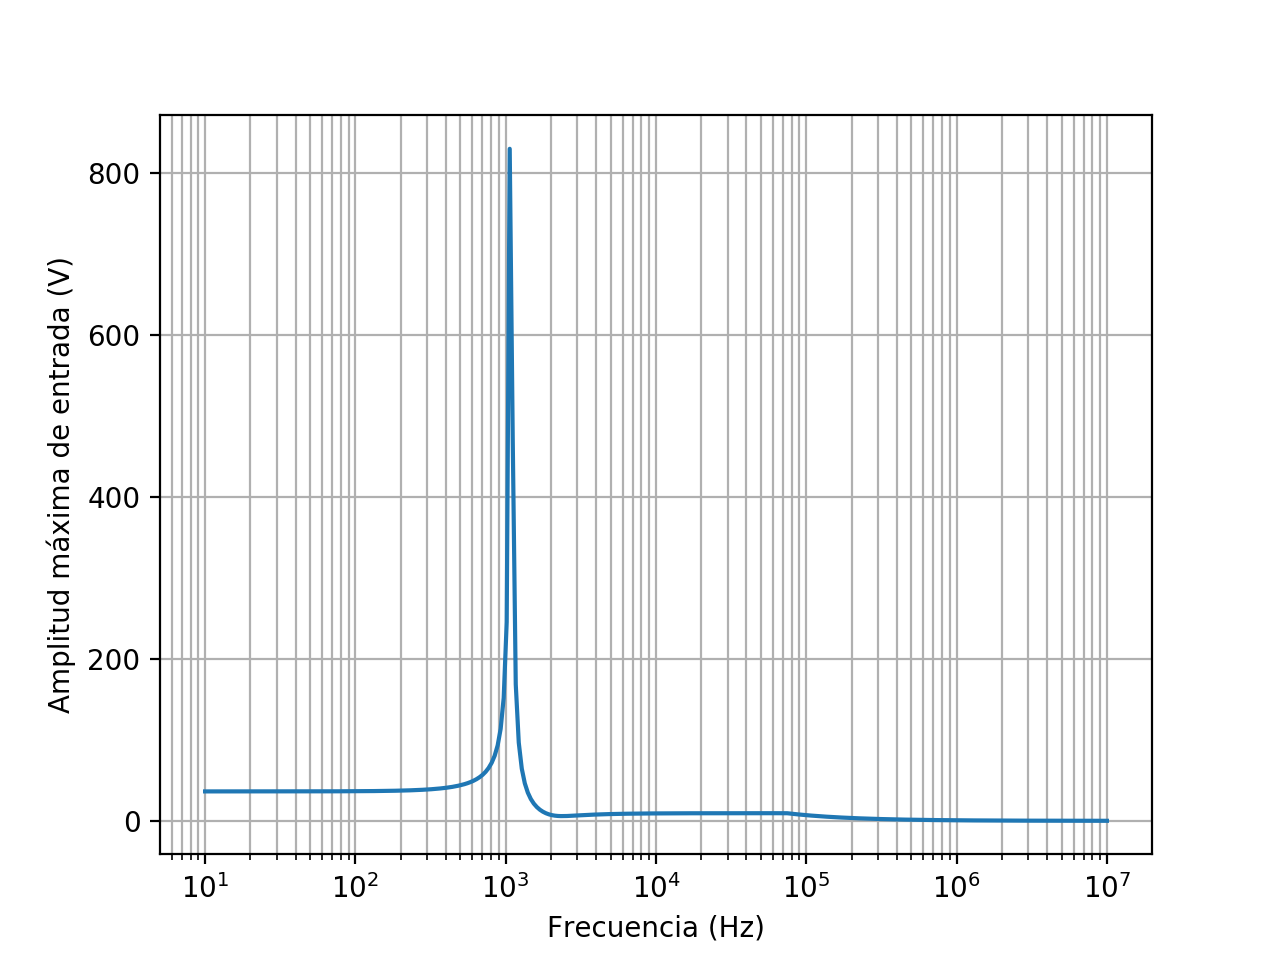
\includegraphics[width=10cm,height=10cm,keepaspectratio]{../EJ1/00GRAFICOS/vinmaxtotal.png}
	\caption{Tensi\'on m\'axima de entrada limitada por slew rate y saturaci\'on.}
	\label{vinmaxtotal}
\end{figure}

En el gr\'afico \ref{vinmaxtotal} se puede ver que la forma que presenta la curva correspondiente a la tensi\'on de entrada m\'axima al circuito respecto a la frecuencia, es inversa a aquella de la funci\'on transferencia. Esto se debe a que al tratarse de un high pass notch, donde hay ganancia de tensi\'on, disminuye la tensi\'on m\'axima de entrada ya que la misma puede saturar al superar la tensi\'on de Vcc. Cerca de la frecuencia del pico del notch, al haber mucha atenuaci\'on, la tensi\'on m\'axima de entrada aumenta enormemente ya que igual ser\'a atenuada al ingresar al ciruito.



\subsection{Conclusiones}
Es importante remarcar de esta parte del trabajo pr\'actico, c\'omo los valores de los componentes afectan al comportamiento del circuito. Se pudo ver que variando la $R_8$ el circuito deja de funcionar como un high pass notch. Al variar $R_1$ o $R_3$ se desplaza hacia la derecha o horizontalmente el pico del notch. Hay ciertos componentes que por la sensibilidad que tiene el Q frente a ellos, son los elegidos en caso de querer variar dicho par\'ametro del circuito. Estos son algunos ejemplos sobre los an\'alisis ellos anteriormente. Si bien se podr\'ian haber elegido componentes para disminuir los efectos de las sensibilidades m\'as que en el caso implementado, no se hizo ya que las especificaciones de dise\~no solicitadas pr\'acticamente determinaban los valores de los componentes sin mucha libertad. Es decir, no siempre se podr\'a elegir lo mejor en cuanto a las sensibilidades ya que si se necesitan cumplir ciertos requerimientos, no ser\'ia correcto pasarlos por algo para mejorar otra cosa. Por \'ultimo, queda pendiente encontrar un buen m\'etodo que permita medir impedancia de salida de forma convincent.

	\newpage
	\section{Ejercicio 2: Introducci\'on al dise\~no de filtros}
En esta secci\'on se propone el dise\~no de cuatro filtros de segundo orden, cada uno de un diferente tipo,
ya sea un pasabajo, pasaalto, pasabanda y rechazabanda. El objetivo de tal dise\~no es encontrar una funci\'on matem\'atica
que desde un punto de vista te\'orico modele o describa a los filtros, y luego analizar su implementaci\'on a trav\'es del uso de lo que se
denomina un Gyrator, lo cual ser\'a abordado y explicado posteriormente. Se establecen como criterios de dise\~no para los filtros la siguiente tabla:

\begin{table}[H]
    \centering
    \begin{tabular}{c c c c}
        Tipo de filtro & $f_p [Hz]$ & $f_a [Hz]$ & $f_c [Hz]$ \\
        \hline \\
        Pasabajos & $3kHz$ & $10.5kHz$ & $-$ \\
        Pasaaltos & $3.5kHz$ & $1kHz$ & $-$ \\
        Pasabanda & $-$ & $-$ & $6kHz$ \\
        Rechazabanda & $-$ & $-$ & $1kHz$ \\
        \hline
    \end{tabular}
    \caption{Condiciones de dise\~no}
\end{table}

En el caso particular de los filtros pasabajos y pasaaltos, se requiere que las bandas pasantes se encuentren por encima de los $-3dB$ y las bandas de rechazo por debajo
de los $-10dB$.

Una vez se haya obtenido los desarrollos te\'oricos para fundamentar las implementaciones de cada uno de los circuitos requeridos, se los simular\'a e
implementar\'a pr\'acticamente, para poder contrastar los comportamientos en estos diferentes contextos, con el fin de evaluar el resultado obtenido.

\subsection{Introducci\'on Te\'orica}
El objetivo de esta introducci\'on te\'orica es presentar brevemente algunos conceptos \'utiles para comprender el an\'alisis realizado posteriormente a lo largo del desarrollo.

\subsubsection{Filtros de segundo orden}
Para los prop\'ositos del desarrollo a realizar, se entiende un filtro como un sistema descripto por una funci\'on transferencia $H(s)$ que se asume lineal, de tiempo invariante
y bibo-estable, tal que su respuesta en frecuencia $H(f)$ modula en amplitud y fase las se\~nales de entrada, produciendo efectos diferenciados seg\'un la frecuencia de las mismas. Por ende,
se puede realizar una clasificaci\'on de tipos de filtros seg\'un la forma en la cual la respuesta en frecuencia del sistema modula las se\~nales de entrada. Usualmente para describir a los filtros se toman
frecuencias cr\'iticas o de referencia denominadas frecuencias de corte, en donde cambia la curva de respuesta.

\begin{itemize}
    \item Filtros pasabajos: Aten\'uan \'unicamente para frecuencias superiores a la frecuencia de corte.
    \item Filtros pasaaltos: Aten\'uan \'unicamente para frecuencias inferiores a la frecuencia de corte.
    \item Filtros pasabanda: Aten\'uan todas las frecuencias exceptuando un rango de frecuencias en torno a la frecuencia de corte.
    \item Filtros rechazabanda: Aten\'uan para un rango de frecuencias en torno a la frecuencia de corte.
\end{itemize}

\subsubsection{Gyrator}

\begin{figure}[H]
    \centering
    \includegraphics[scale=0.7]{../EJ2/Recursos/gyrator.png}
    \caption{Modelo del Gyrator}
    \label{fig:gyrator_modelo}
\end{figure}

El Gyrator es un dispositivo que inicialmente surgi\'o como un modelo te\'orico caracterizado por ser un cuadripolo no rec\'iproco con par\'ametros de impedancia
descriptos como se muestra en la expresi\'on de la Ec. \ref{eq:parametros_gyrator}. La funci\'on principal de un Gyrator es la de girar o invertir una impedancia, permitiendo
de esta forma simular la presencia de componentes inductivos a partir de componentes capacitivos, lo cual era buscado ya que la implementaci\'on real de un inductor a trav\'es de una bobina
no tiene un buen rendimiento para bajas frecuencias, suelen ser elementos grandes y funcionan bien para una frecuencia particular de construcci\'on.

\begin{equation*}
    \begin{pmatrix}
        V_1 \\ V_2
    \end{pmatrix}
    =
    \begin{pmatrix}
        0 & -r \\
        r & 0
    \end{pmatrix}
    \cdot 
    \begin{pmatrix}
        I_1 \\ -I_2
    \end{pmatrix}
    \label{eq:parametros_gyrator}
\end{equation*}

Existen diversas configuraciones en las cuales un amplificador operacional permite implementar un circuito de Gyrator, en la Fig. \ref{fig:circuito_gyrator} se ilustra una de ellas
empleando \'unicamente un s\'olo amplificador. El objetivo de este circuito en particular es simular un comportamiento inductivo como impedancia de entrada al circuito, a partir de algunas resistencias y un capacitor.

\begin{figure}[H]
    \centering
    \includegraphics[scale=0.6]{../EJ2/Recursos/circuito_gyrator.png}
    \caption{Circuito Gyrator con un amplificador operacional}
    \label{fig:circuito_gyrator}
\end{figure}

Para comprender en detalle el funcionamiento del circuito se lo estudia desde diferentes enfoques. Es importante aclarar que todo an\'alisis realizado tiene en cuenta condiciones ideales,
dado que cualquier apreciaci\'on de las caracter\'isticas no ideales del circuito ser\'a realizada durante las implementaciones para estudiar el rango de operaci\'on donde son v\'alidos los criterios ideales.

\paragraph*{An\'alisis circuital: } Desde un punto de vista circuital, analizando al circuito como un cuadripolo al cual se busca la impedancia de entrada $Z_{IN} = \frac{V_{IN}}{I_{IN}}$, se considera inicialmente un amplificador operacional ideal en una configuraci\'on conocida como seguidor de tensi\'on o buffer.

\begin{eqnarray*}
    I_{IN} & = I_L + I_C \\
    I_C & = \frac{V_{IN}}{R_C + \frac{1}{s \cdot C}} \\
    I_L & = \frac{V_{IN}}{R_L} \cdot \frac{1}{1 + s \cdot C \cdot R}
\end{eqnarray*}

\begin{equation}
    \Rightarrow Z_{IN} = \frac{V_{IN}}{I_{IN}} = \frac{R_L + s \cdot C \cdot R_C \cdot R_L}{1 + s \cdot C \cdot R_L}
\end{equation}

Resulta interesante que tal circuito tiene una representaci\'on equivalente que puede ser demostrada llegando en ambos casos a la misma impedancia de entrada,
desde un punto de vista ideal puede ser empleado tal modelo equivalente para el dise\~no de los circuitos deseados. En la Fig. \ref{fig:equivalente_gyrator} se ilustra tal modelo equivalente para el circuito propuesto.

\begin{figure}[H]
    \centering
    \includegraphics[scale=0.6]{../EJ2/Recursos/equivalente_gyrator.png}
    \caption{Circuito equivalente para el Gyrator con un opamp}
    \label{fig:equivalente_gyrator}
\end{figure}

\begin{equation}
    Z_{IN} = \frac{V_{IN}}{I_{IN}} = (s \cdot C \cdot R_C \cdot R_L + R_L) // (\frac{1 + s \cdot R_C \cdot C}{s \cdot C})
    \Rightarrow Z_{IN} = \frac{R_L \cdot (1 + s \cdot C \cdot R_C)}{1 + s \cdot C \cdot R_L}
\end{equation}

En una primera instancia, el an\'alisis que podr\'ia realizarse de este circuito es que si se considera una dada frecuencia de corte 
$\omega_o = \frac{1}{C \cdot R_L}$, luego puede establecerse que para frecuencias que cumplan ser $\omega << \omega_o \Rightarrow \frac{\omega}{\omega_o} << 1$ y bajo esta consideraci\'on
ser\'ia posible caracterizar al circuito como una bobina, donde la impedancia de entrada se puede aproximar como $Z_{IN} = R_L + s \cdot C \cdot R_C \cdot R_L$. Este an\'alisis final busca ver en el Gyrator condiciones para las cuales pueda ser pensado como lo que dio inicio a la b\'usqueda de este circuito, que es la simulaci\'on de un inductor, m\'as all\'a de que con la aproximaci\'on tomada
el resultado haya sido una bobina de inductancia equivalente $L = C \cdot R_C \cdot R_L$ y factor de calidad $Q = \omega \cdot R_C \cdot C$.

\paragraph*{An\'alisis del circuito realimentado:} si bien pudieron obtenerse resultados concretos del an\'alisis circuital del Gyrator, se buscan otros enfoques
para obtener una mayor comprensi\'on del funcionamiento de este circuito. 

En un principio, si se observa nuevamente el circuito de la Fig. \ref{fig:circuito_gyrator} e imaginariamente se desconecta el buffer y la resistencia $R_L$, lo que se tiene es un circuito simple RC,
no obstante al agregar la otra parte de la configuraci\'on se crea una realimentaci\'on dentro del circuito. Consid\'erese este sistema donde inicialmente s\'olo se posee la rama de $C$ y $R_C$ y asumiendo valores arbitrarios la corriente por dicha rama se encuentra en el primer cuadrante por su car\'acter capacitivo, luego cuando
se conecta el lazo, el mismo agrega una componente de corriente a la total que es proporcional a la $I_C$ pero se encuentre en contrafase. Esto \'ultimo produce constamente un desplazamiento de la corriente
total desde el $1^{\circ}$ al $4^{\circ}$ cuadrante. Esto mismo se puede observar en el diagrama fasorial con valores arbitrarios de la Fig. \ref{fig:fasores_gyrator}. Bajo las condiciones donde ese cambio de cuadrante en la corriente implique un cambio en su fase de positivo a negativo,
implicar\'a que la impedancia de entrada se vio invertida del comportamiento capacitivo al inductivo.

\begin{figure}[H]
    \centering
    \includegraphics[scale=0.8]{../EJ2/Recursos/fasores_gyrator.png}
    \caption{Diagrama fasorial para caracterizar la inversi\'on de impedancia del Gyrator}
    \label{fig:fasores_gyrator}
\end{figure}

Luego pasando a un an\'alisis m\'as cuantitativo del sistema realimentado, consid\'erese al sistema caracterizado por su impedancia de entrada, para lo cual se modeliza al mismo con entrada de corriente $I_{IN}$ y salida en $V_{IN}$,
entonces partiendo de las ecuaciones ya empleadas en el an\'alisis circuital, se puede considerar el siguiente diagrama en bloques del sistema a lazo cerrado, ilustrado en la Fig. \ref{fig:sistema_gyrator}.

\begin{figure}[H]
    \centering
    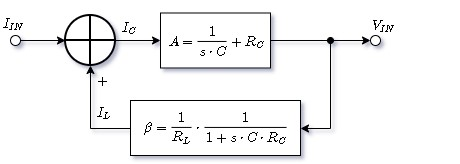
\includegraphics[scale=0.7]{../EJ2/Recursos/sistema_gyrator.jpg}
    \caption{Sistema a lazo cerrado del circuito Gyrator propuesto}
    \label{fig:sistema_gyrator}
\end{figure}

Se caracteriza la funci\'on transferencia, es decir la impedancia de entrada del circuito, en t\'erminos generales se llega a que:

\begin{equation}
    Z_{IN}(s) = \frac{A}{1 + \beta \cdot A}
\end{equation}

Particularmente para los casos donde, como suele suceder con los sistemas a lazo cerrado, la magnitud de $A >> 1$, entonces se puede aproximar
la funci\'on como:

\begin{equation}
    Z_{IN}(s) \approx \frac{1}{\beta} = R_L + s \cdot C \cdot R_C \cdot R_L
\end{equation}

Estudiando al Gyrator como el sistema realimentado que se propuso aqu\'i, resulta evidente una posible interpretaci\'on f\'isica del l\'imite superior en frecuencia
hasta el cual funciona tal configuraci\'on. Este l\'imite que fue definido por el capacitor $C$ y la resistencia $R_L$ influye en el hecho de que el funcionamiento del sistema se encuentre en torno
a la realimentaci\'on de corriente en contrafase que permite invertir el fasor y simular un comportamiento inductivo a partir de uno capacitivo. Es por esto \'ultimo que para las frecuencias donde la impedancia del capacitor se vuelva despreciable, luego 
 la componente capacitiva habr\'a disminuido consecuentemente la componente inductiva tambi\'en lo har\'a.
Por otro lado, la resistencia $R_L$ influye porque es lo que define la constante proporcional entre lo que se mide y lo que se inyecta, si fuera demasiado grande  la corriente inyectada no ser\'ia suficiente para invertir la fase.

\paragraph*{Gyrator con referencia a generador:} Para terminar con este an\'alisis te\'orico del Gyrator, es importante observar que el circuito estudiado tiene una impedancia equivalente
que bajo ciertas condiciones coincide con la de una bobina, pero se encuentra en referencia con masa. Esto \'ultimo puede ser un inconveniente en circuitos donde se busca utilizar una bobina flotante,
pero para ello desde un punto de vista te\'orico se necesitar\'ian dos Gyrators o circuitos m\'as complejos.

Por otro lado, la implementaci\'on de algunos filtros en configuraci\'on RLC requieren que la bobina se encuentre en la rama serie, y como no se tiene la posibilidad de fabricar una bobina flotante,
se propone conectar el circuito referenciado al generador y estudiar si esta configuraci\'on puede resultar beneficiosa. Se propone entonces, estudiar el circuito de la Fig. \ref{fig:circuito_gyrator_referencia_generador}.

\begin{figure}[H]
    \centering
    \includegraphics[scale=0.65]{../EJ2/Recursos/gyrator_referenciado_generador.png}
    \caption{Circuito Gyrator con referencia a generador}
    \label{fig:circuito_gyrator_referencia_generador}
\end{figure}

Se estudiar\'a el circuito analiz\'andolo al mismo como un dipolo activo que se compone del conjunto generador y gyrator,
de esta forma se buscan los par\'ametros de la impedancia de Thevenin o salida, as\'i como su tensi\'on de Thevenin correspondiente. Para esto \'ultimo,
se plantea un sistema de ecuaciones que caracteriza al circuito y se lo resuelve:

\begin{align*}
    & V_p = \frac{V_o \cdot (R_G + R_C)}{R_G + R_C + \frac{1}{s \cdot C}} + \frac{V_i \cdot \frac{1}{s \cdot C}}{R_G + R_C + \frac{1}{s \cdot C}} \\
    & A_{vol} = \frac{GBP}{s + \omega_p} \\
    & V_n = (V_p - V_n) \cdot A_{vol} \\
    & V_o = \frac{(V_p - V_n) \cdot R_L}{R_L + \frac{1}{s \cdot C}} + V_n
\end{align*}

Entonces, operando correctamente sobre estas expresiones se puede llegar a que la tensi\'on de Thevenin ser\'a:

\begin{equation}
    V_{TH} = V_i \cdot \frac{GBP}{GBP + \omega_p} \cdot
    \frac{s^{2} \cdot \frac{C \cdot R_L}{GBP} + s \cdot \frac{C \cdot R_L \cdot (GBP + \omega_p)}{GBP} + 1}
    {s^{2} \cdot \frac{C \cdot (R_C + R_G + R_L)}{GBP + \omega_p} + s \cdot \left[ 1 + \frac{C \cdot \omega_p \cdot (R_C+ R_G + R_L)}{GBP + \omega_p}  + \frac{C \cdot GBP \cdot R_L}{GBP + \omega_p}\right] + 1}
\end{equation}

En primer lugar, se considera que $GBP >> \omega_p \Rightarrow GBP + \omega_p \approx GBP$. Luego, $\frac{GBP}{GBP+\omega_p} \approx 1$. Por otro lado, reutilizando la condici\'on empleada para aproximar el funcionamiento del Gyrator en el an\'alisis con referencia a masa, donde se denomin\'o
una frecuencia $\omega_o = \frac{1}{C \cdot R_L}$, se opera en frecuencias mucho m\'as bajas y resulta que $\frac{\omega}{\omega_o} << 1$. Partiendo de esto \'ultimo,
adem\'as si se considera que $R_G << R_C < R_L$ entonces se puede considerar que $\frac{\omega^{2}}{GBP \cdot \frac{1}{C \cdot(R_C + R_L)}} << 1$. De esta forma se puede concluir que, bajo la consideraci\'on de estas aproximaciones,
entonces:

\begin{equation}
    V_{TH} \approx V_i
\end{equation}

Y si se analiza la impedancia de Thevenin, o de salida del circuito, implica pasivar al generador y utilizar un generador de prueba $V_{op}$ en la salida, donde la impedancia que se ver\'ia
es la que ya se analiz\'o inicialmente en el circuito del Gyrator referenciado a masa, por lo tanto si adem\'as se incluyen las consideraciones anteriores:

\begin{equation}
    Z_{TH} \approx R_L + s \cdot C \cdot R_C \cdot R_L
\end{equation}

\begin{figure}[H]
    \centering
    \includegraphics[scale=0.5]{../EJ2/Recursos/equivalente_gyrator_referenciado_generador.png}
    \caption{Equivalente del Gyrator referenciado a generador}
    \label{fig:equivalente_referenciado}
\end{figure}

\begin{figure}[H]
    \centering
    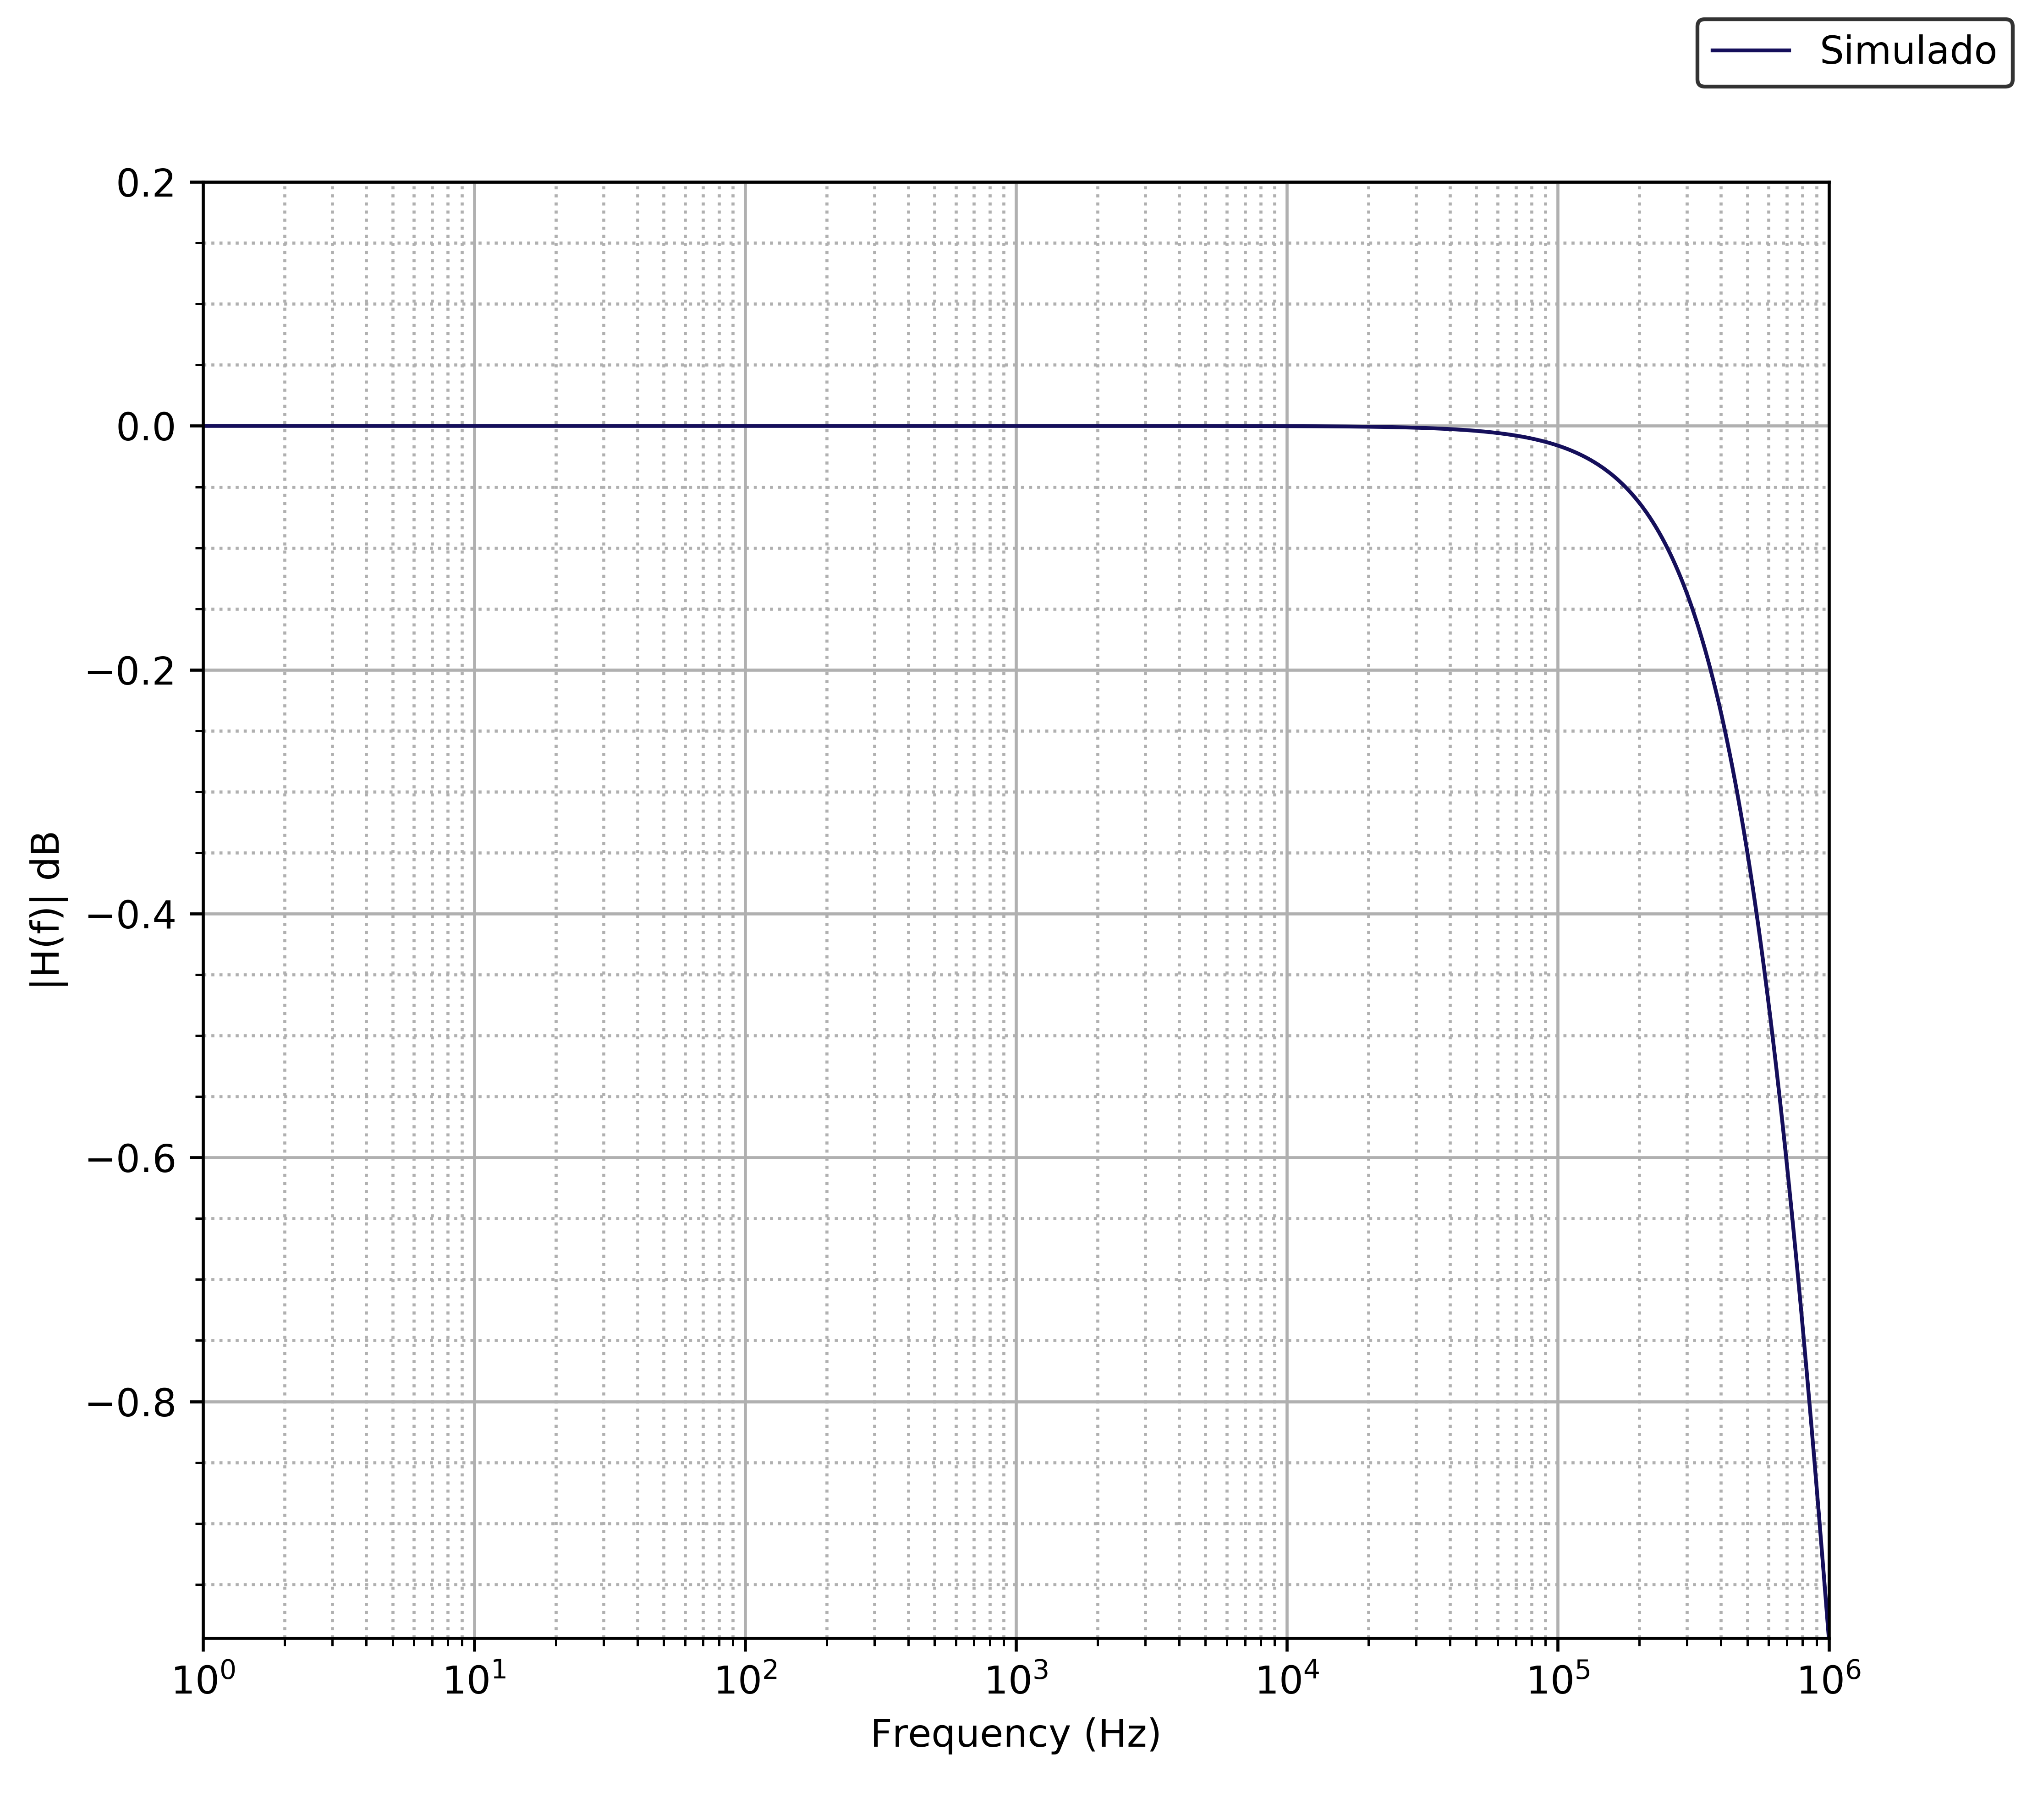
\includegraphics[scale=0.5]{../EJ2/Recursos/gyrator_simulado.png}
    \caption{Simulaci\'on de $H(s) = \frac{V_{TH}}{V_i}$}
    \label{fig:resultados_gyrator_referenciado}
\end{figure}

Finalmente, como se puede observar en la Fig. \ref{fig:resultados_gyrator_referenciado}, efectivamente bajo las apreciaciones realizadas
puede emplearse el modelo equivalente propuesto. Lo que se ilustra es la simulaci\'on del circuito completo para valores arbitrarios de componentes,
pues \'unicamente es de inter\'es mostrar que hasta una frecuencia dada el comportamiento es el aproximado.

\subsection{Filtro Pasabajos}

\subsubsection{Dise\~no de funci\'on transferencia}
Consid\'erese un sistema de segundo orden lineal, de tiempo invariante y bibo-estable, donde se propone para un filtro pasabajos la Ec. \ref{eq:funcion_pasabajos}.

\begin{equation}
    H(s) = \frac{V_o(s)}{V_i(s)} = \frac{1}{1 + \frac{s}{\omega_o \cdot Q} + \left( \frac{s}{\omega_o}\right)^{2}}
    \label{eq:funcion_pasabajos}
\end{equation}

En un principio el sistema propuesto
puede estar dado como un subamortiguado, cr\'iticamente amortiguado o un sobreamortiguado. Se descarta la posibilidad de que se encuentre subamortiguado ya que presentar\'ia un sobrepico en un entorno de la frecuencia de corte
que modificar\'ia el comportamiento buscado, por otro lado se busca que idealmente sea un cr\'iticamente amortiguado porque de esa forma tiene una pendiente de decrecimiento mayor. Para tal caso, el sistema presenta dos polos reales e iguales, ubicados en $\omega_o$. De esta forma se reduce la expresi\'on a la forma:

\begin{equation}
    H(s) = \frac{1}{\left(1 + \frac{s}{\omega_o}\right)^{2}}
    \label{eq:funcion_pasabajos_ideal}
\end{equation}

Para cumplir con la plantilla del filtro requerido, se eval\'ua en las frecuencias pasante y atenuante y se toma $1dB$ de margen respecto de lo consignado.

\begin{eqnarray*}
    & |H(\omega_p)|dB \geq -2dB \Rightarrow 20 \cdot \log{\left(\frac{1}{1 + \left(\frac{\omega_p}{\omega_o}\right)^{2}}\right)} \geq -2dB\\
    & \Rightarrow \omega_o \geq 2\pi \cdot 5.9kHz
\end{eqnarray*}

\begin{eqnarray*}
    & |H(\omega_a)|dB \leq -11dB \Rightarrow 20 \cdot \log{\left(\frac{1}{1 + \left(\frac{\omega_a}{\omega_o}\right)^{2}}\right)} \leq -11dB \\
    & \Rightarrow \omega_o \leq 2 \pi \cdot 6.57kHz
\end{eqnarray*}

Por lo tanto, si se ubica la frecuencia de corte dentro del rango $5.9kHz < f_o < 6.57kHz$ luego se puede garantizar que se cumple con la plantilla. Si se lo ubica en el valor medio del rango,
se logra que ante cualquier variaci\'on por la dispersi\'on de las caracter\'isticas de los componentes tenga el mayor margen de forma sim\'etrica. 
Entonces $f_o = \frac{5.9kHz + 6.57kHz}{2} = 6.235kHz$. Desde este punto de vista, la m\'axima variaci\'on para la frecuencia de corte sin que se salga de lo requerido,
est\'a dado como $\Delta f = \frac{6.57kHz - 5.9kHz}{2} = 370Hz$, por lo tanto la frecuencia de corte puede desviarse un $5\%$ aproximadamente. Lo cual si bien no es tan amplio como se quisiera, hay que recordar
que se parte de sobredimensionamientos iniciales.

\subsubsection{Dise\~no de circuito con Gyrator}
Desde un punto de vista matem\'atico se encontr\'o que la Ec. \ref{eq:funcion_pasabajos_ideal} describe un sistema que se comporta como un filtro pasabajos. En general, en el dise\~no de filtros an\'alogicos pasivos se utilizar\'ia un circuito RLC . No obstante, como bien se mencion\'o con anterioridad, en la pr\'actica para bajas frecuencias no suele utilizarse un inductor por su tama\~no y limitado rango de funcionamiento,
adem\'as de los efectos par\'asitos que suele traer consigo. Por esto mismo, se utilizar\'a el circuito Gyrator.

En rasgos generales, el proceso de dise\~no consiste inicialmente en proponer una configuraci\'on con el circuito Gyrator con la cual pueda llegarse a una funci\'on transferencia deseada,
luego utilizando un an\'alisis ideal determinar los valores de componentes y, finalmente, realizar un an\'anisis no ideal para determinar condiciones de operaci\'on o limitaciones sobre
el amplificador operacional, para que se cumpla lo mayor posible el resultado ideal.

\paragraph*{Circuito equivalente aproximado:} Considerando que con un Gyrator bajo ciertas condiciones se puede simular un inductor con una resistencia en serie, si se agrega un capacitor adicional puede armarse un simple circuito RLC para el filtro,
por tanto se analiza el circuito que se ilustra en la Fig. \ref{fig:equivalente_gyrator}. Consid\'erese que en la determinaci\'on de los valores de componentes se establecer\'a $R_L >> R_G$ con lo cual el efecto de 
la resistencia del generador puede despreciarse y no produce una desviaci\'on notable. 

\begin{figure}[H]
    \centering
    \includegraphics[scale=0.6]{../EJ2/Recursos/equivalente_pasabajos.png}
    \caption{Circuito pasabajos equivalente}
    \label{fig:equivalente_pasabajos}
\end{figure}

\begin{eqnarray*}
    & H(s) = \frac{V_o(s)}{V_i(s)} = \frac{ \frac{1}{s \cdot C_2} }{ s \cdot L + R_L + \frac{1}{s \cdot C_2}} = \frac{1}{s^{2} \cdot L \cdot C + s \cdot C_2 \cdot R_L + 1} \\
    & \Rightarrow \omega_o = \frac{1}{\sqrt{(LC)}} \Rightarrow L = \frac{1}{C_2 \cdot (2\pi \cdot 6.235kHz)^{2}} \\
    & \Rightarrow \xi = 1 \rightarrow C_2 \cdot R_L = \frac{2}{\omega_o} \Rightarrow R_L = \frac{1}{\pi \cdot 6.235kHz \cdot C_2}
\end{eqnarray*}

Parametrizando los valores de componentes en funci\'on del capacitor de salida, luego se puede determinar un valor de capacidad el cual sea lo suficientemente grande para que no se vea afectado
por capacidades par\'asitas o capacidades correspondientes a las puntas de medici\'on del osciloscopio, con lo cual utilizando $C_2 = 33nF$ luego se obtiene que $R_L = 1.5k \Omega$ y $L = 19.74mH$.

\paragraph*{Circuito completo:} En la Fig. \ref{fig:circuito_gyrator} se ilustra el esquema completo del circuito implementado con un Gyrator, donde se aplican los criterios ya considerados en el an\'alisis del Gyrator con referencia en el generador.

Respetando la condici\'on dada por el hecho de que se defin\'ia una frecuencia angular $\omega_o = \frac{1}{C \cdot R_L}$ y se estableci\'o que el comportamiento inductivo se dar\'ia siempre y cuando $\omega << \omega_o$,
se adopta como criterio que $f_o \geq 10 \cdot f_a = 100,5kHz$, es decir, una d\'ecada despu\'es de la frecuencia atenuante.

\begin{eqnarray}
    & C_{max} = \frac{1}{\omega_{o_{min}} \cdot R_L} = \frac{1}{1.5k \Omega \cdot 2\pi \cdot 100.5kHz} = 1.05nF\\
    & R = \frac{1}{C \cdot R_L} \Rightarrow C = 470pF \rightarrow R = 28k \Omega = 56k\Omega // 56k\Omega
\end{eqnarray}

\begin{figure}[H]
    \centering
    \includegraphics[scale=0.5]{../EJ2/Recursos/circuito_pasabajos.png}
    \caption{Circuito completo pasabajos con Gyrator}
    \label{fig:circuito_pasabajos}
\end{figure}

\paragraph*{An\'alisis no ideal:} Considerando que el amplificador operacional tiene un funcionamiento no ideal, esto es, con un $A_{vol}$ finito y con un polo dominante
a partir del cual decrece tal magnitud, y llamando como $V_A$ al potencial en la salida de dicho amplificador, luego se realiza un an\'alisis planteando las siguientes ecuaciones
sobre el circuito, de las cuales desarroll\'andolas se obtiene finalmente una expresi\'on para la transferencia del circuito sin aproximaciones ni idealidades.

\begin{align}
    & V_p = \frac{V_o \cdot R_2}{R_2 + \frac{1}{s \cdot C_2}} \\
    & A_{vol} = \frac{GBP}{s + \omega_p} \\
    & V_n = (V_p - V_n) \cdot A_{vol} \\
    & \frac{V_i - V_o}{R + \frac{1}{s \cdot C}} = \frac{V_o}{R_2 + \frac{1}{s \cdot C_2}} + \frac{V_o - V_n}{R_L}
\end{align}

\begin{align*}
    & a = \frac{R_L \cdot C}{GBP} \\
    & b = \frac{C \cdot R_L \cdot (GBP + \omega_p)}{GBP} \\
    & \alpha = \frac{C \cdot C_2 \cdot R \cdot R_L}{GBP + \omega_p} \\
    & \beta = \left[ C \cdot C_2 \cdot R \cdot R_L + \frac{C \cdot (R + R_L) + C_2 \cdot R_L}{GBP + \omega_p} \right] \\
    & \gamma = \left[C \cdot \frac{GBP \cdot R_L + R \cdot \omega_p + R_L \cdot \omega_p}{GBP + \omega_p} + C_2 \cdot R_L + \frac{1}{GBP + \omega_p} \right] \\
    & H(s) = \frac{GBP}{GBP + \omega_p} \cdot
    \frac{s^{2} \cdot a + s \cdot b + 1}
    {s^{3} \cdot \alpha + s^{2} \cdot \beta + s \cdot \gamma + 1} 
\end{align*}

Para demostrar que con los valores tomados se puede aproximar el comportamiento al ideal utilizado, debe considerarse que $GBP >> \omega_p$, entonces $\frac{GBP}{GBP + \omega_p} \approx 1$. Luego tomando que $\omega << \frac{1}{C \cdot R_L}$ y $\omega << GBP$, entonces se puede
considerar que el numerador de la funci\'on es $Num[H(s)] \approx 1$. Por otro lado se puede derivar de lo anterior que $\omega^{3} << \frac{GBP + \omega_p}{C_2 \cdot C \cdot R \cdot R_L}$ y asumiento que, dados los valores apropiados, $\frac{1}{C_2 \cdot R_L} << GBP + \omega_p$, entonces se puede aproximar
que la funci\'on transferencia es:

\begin{equation}
    H(s) \approx \frac{1}{s^{2} \cdot C \cdot C_2 \cdot R \cdot R_L + s \cdot C_2 \cdot R_L + 1}
\end{equation}

\subsubsection{Verificaci\'on del dise\~no}
Para el armado del circuito en la pr\'actica se utilizar\'an resistencias de una tolerancia de $1\%$, y capacitores con una tolerancia de $10\%$, esto provoca que en la realidad
pueda haber una dispersi\'on que modifique el resultado final del filtro. Para conocer la posible variaci\'on y asegurar que est\'e dentro de un rango aceptable, se simula en LTSpice
y obtiene la respuesta en frecuencia usando Monte Carlo para variar los componentes. S\'olo se ilustra el m\'odulo del resultado porque no es de inter\'es la fase a los prop\'ositos de estas observaciones. 
Los resultados pueden observarse en las figuras mostradas en \ref{fig:lp_montecarlo} y \ref{fig:lp_montecarlo_frecuencias} y puede observarse que para las frecuencias pasante y atenuante se cumple con los criterios
adoptados en el dise\~no.

\begin{figure}[H]
    \centering
    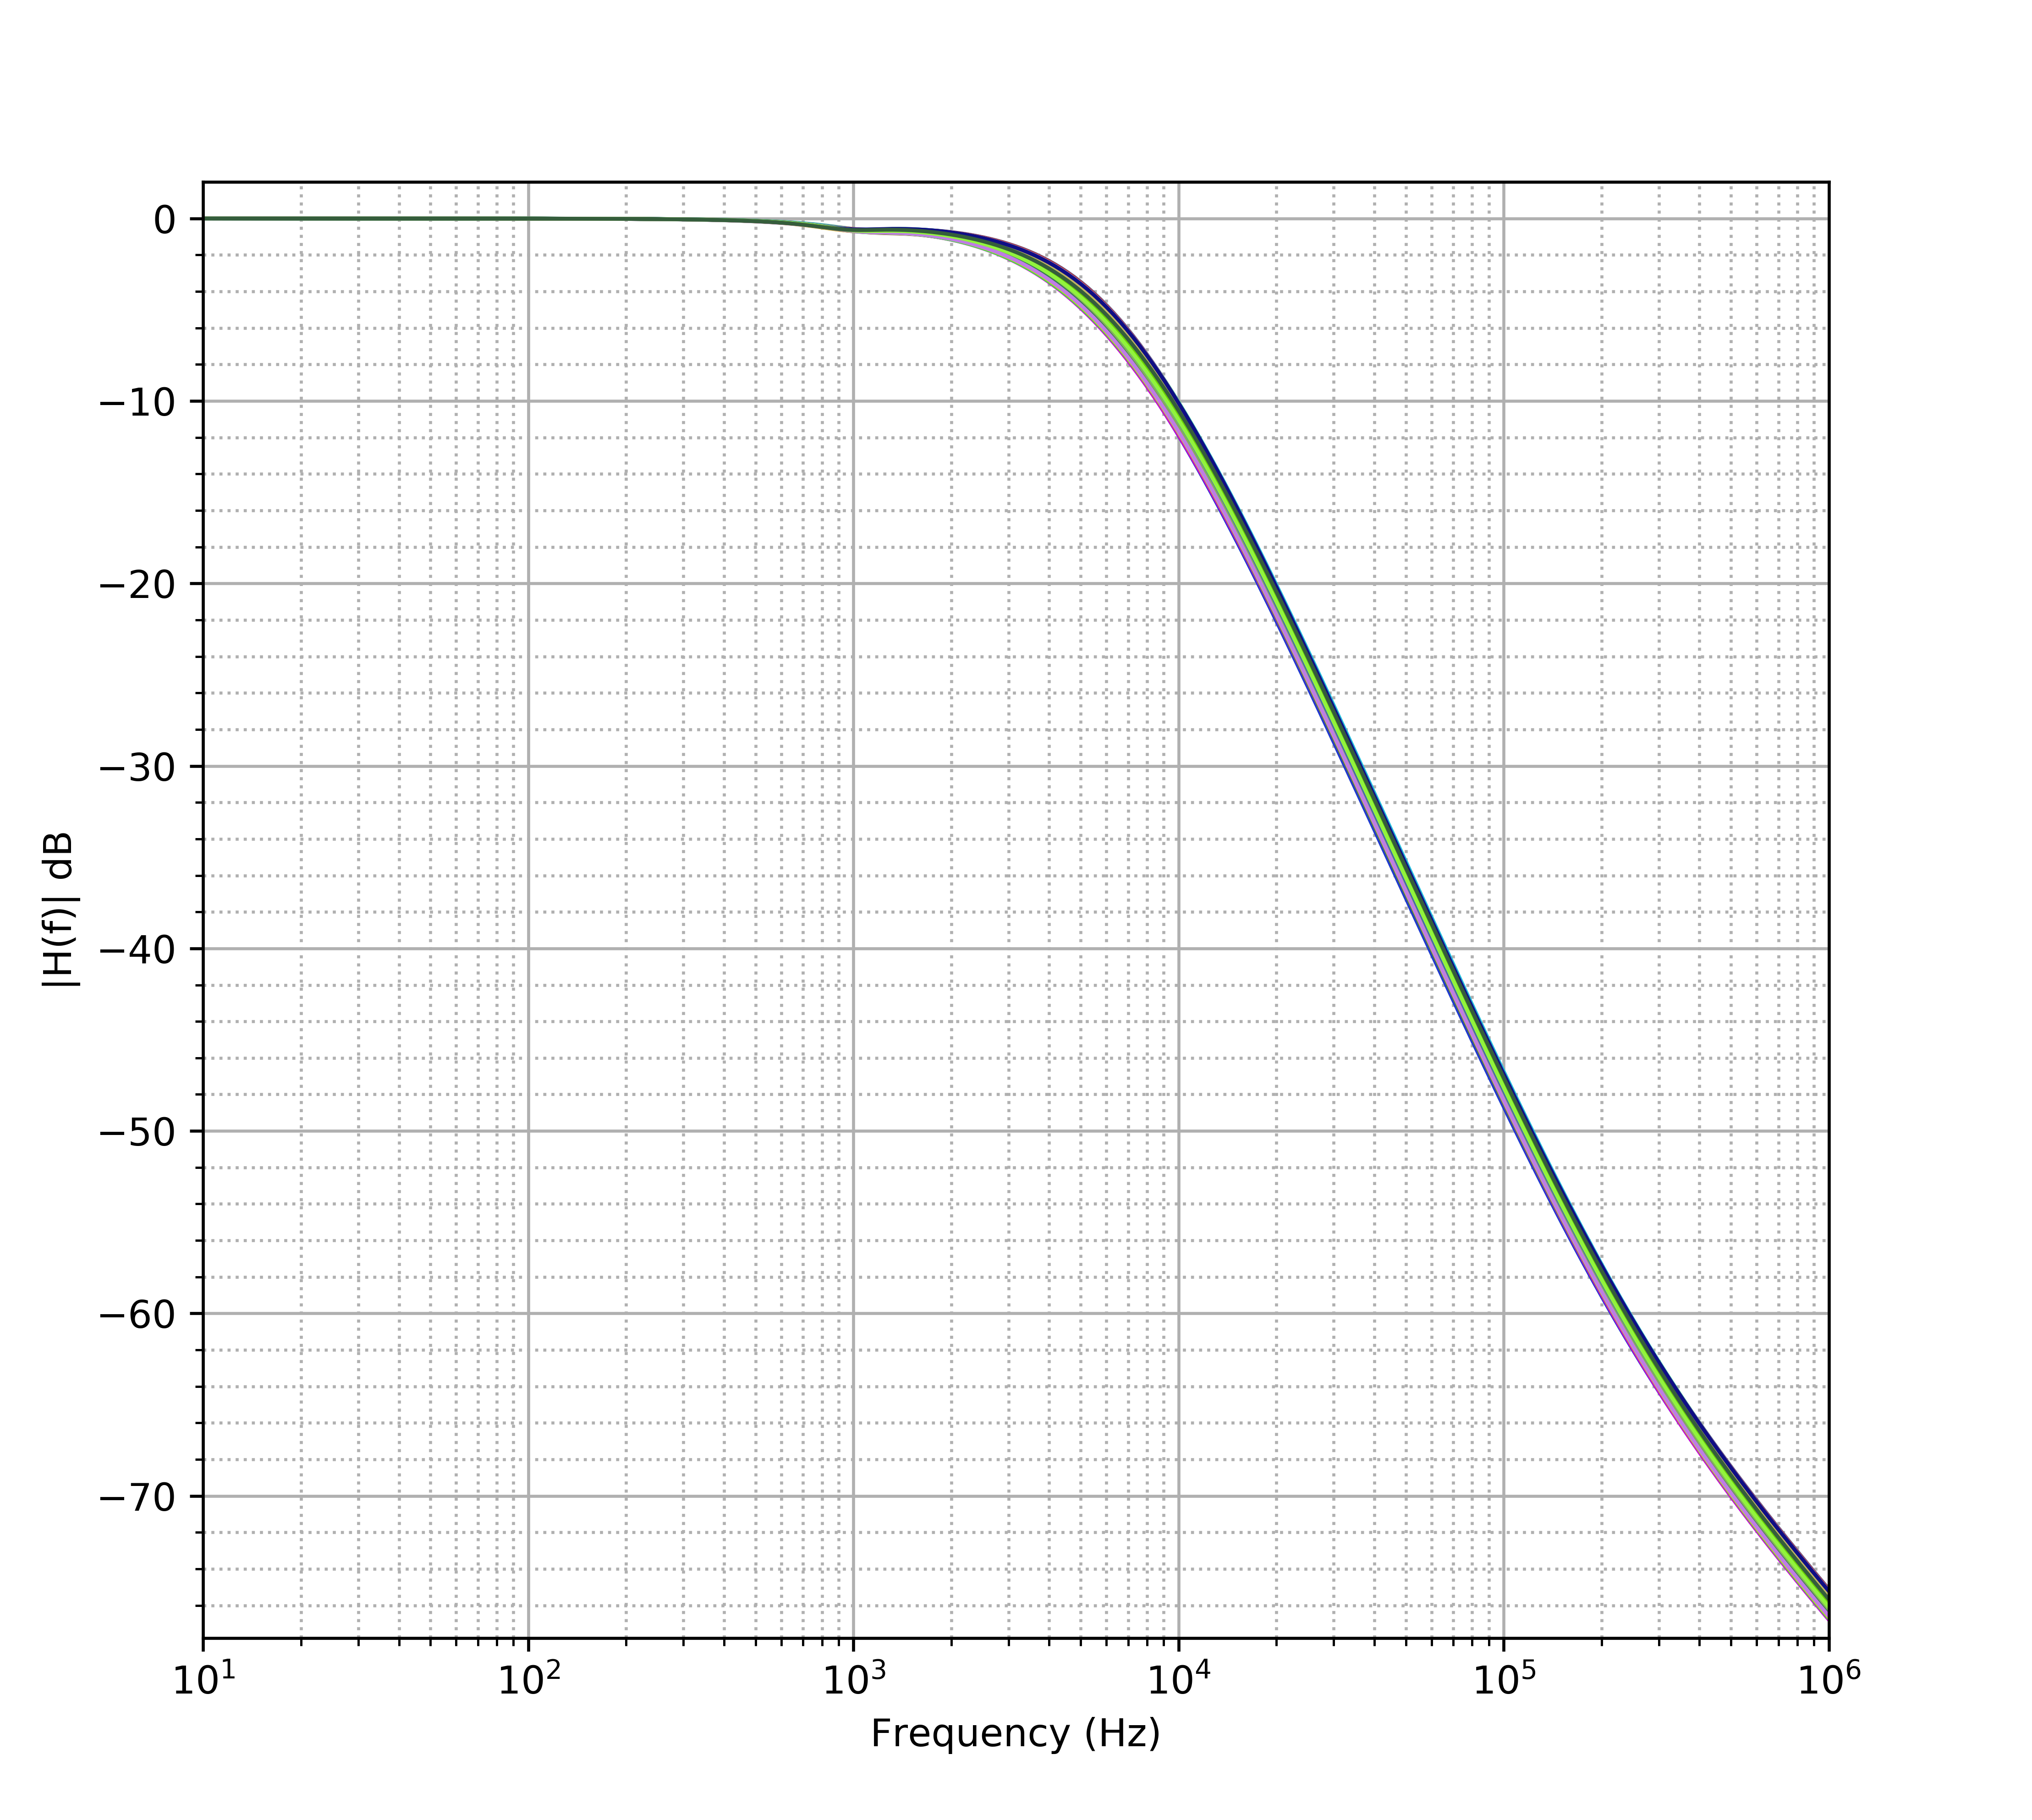
\includegraphics[scale=0.12]{../EJ2/Recursos/lp_montecarlo.png}
    \caption{M\'odulo de la respuesta en frecuencia del filtro pasabajos en escala semilogar\'itmica}
    \label{fig:lp_montecarlo}
\end{figure}

\begin{figure}[H]
    \centering
    \begin{tabular}{c c}
        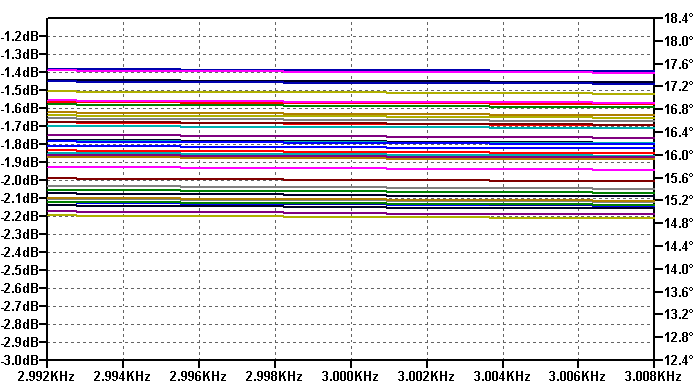
\includegraphics[scale=0.4]{../EJ2/Recursos/lp_montecarlo_fp.png}
        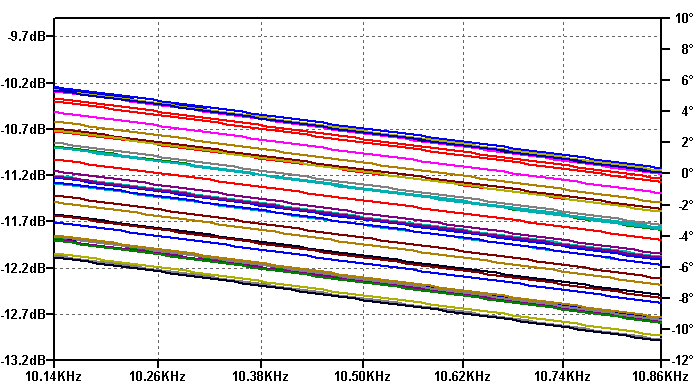
\includegraphics[scale=0.4]{../EJ2/Recursos/lp_montecarlo_fa.png}
    \end{tabular}
    \caption{Vista aumentada en frecuencias pasante y atenuante}
    \label{fig:lp_montecarlo_frecuencias}
\end{figure}

\subsubsection{Resultados}
En las Fig. \ref{fig:bode_pasabajos_modulo} y \ref{fig:bode_pasabajos_fase} se constrastan los resultados te\'oricos, simulados y las mediciones obtenidas sobre la implementaci\'on
pr\'actica del circuito.

Para $f = 3kHz$ se obtuvo que $|H(f)| = -2.7dB$ con una fase de $-53^{\circ}$.

Para $f = 10.5kHz$ se obtuvo que $|H(f)| = -12.4dB$ con una fase de $-117^{\circ}$.


\begin{figure}[H]
    \centering
        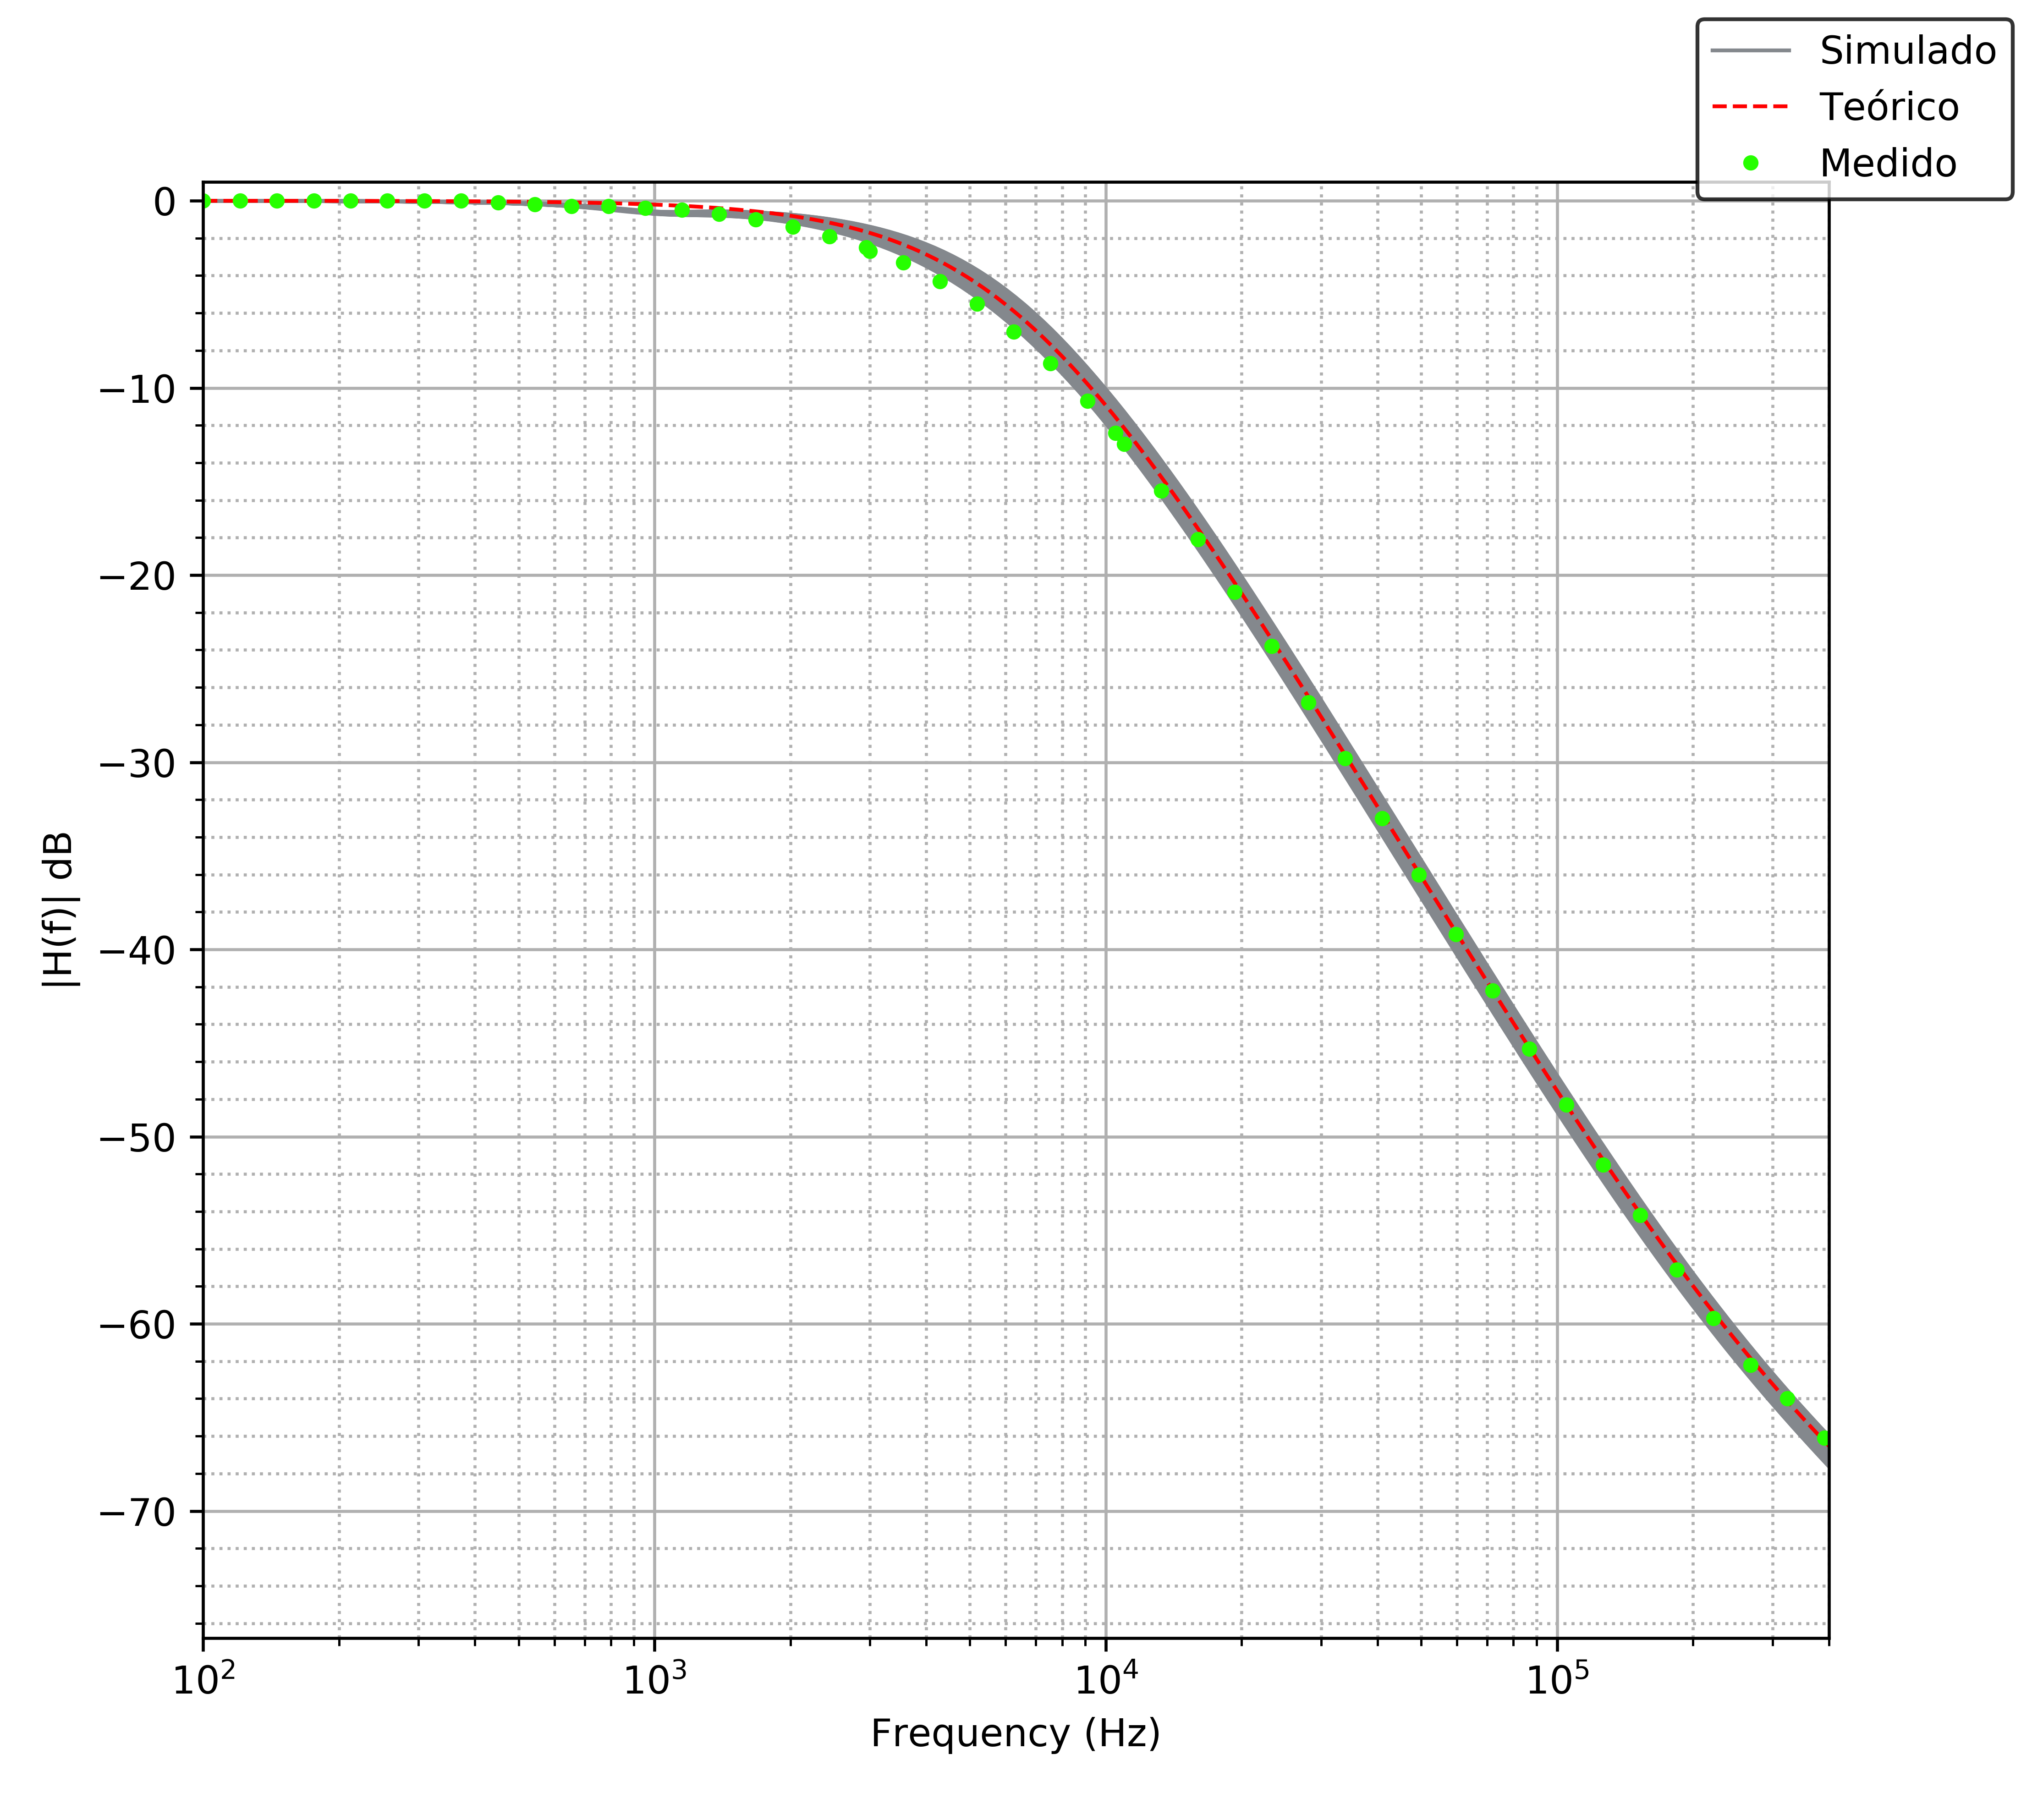
\includegraphics[scale=0.5]{../EJ2/Recursos/bode_pasabajos_modulo.png}
    \caption{Diagrama de bode en m\'odulo del filtro pasabajos}
    \label{fig:bode_pasabajos_modulo}
\end{figure}

\begin{figure}[H]
    \centering
        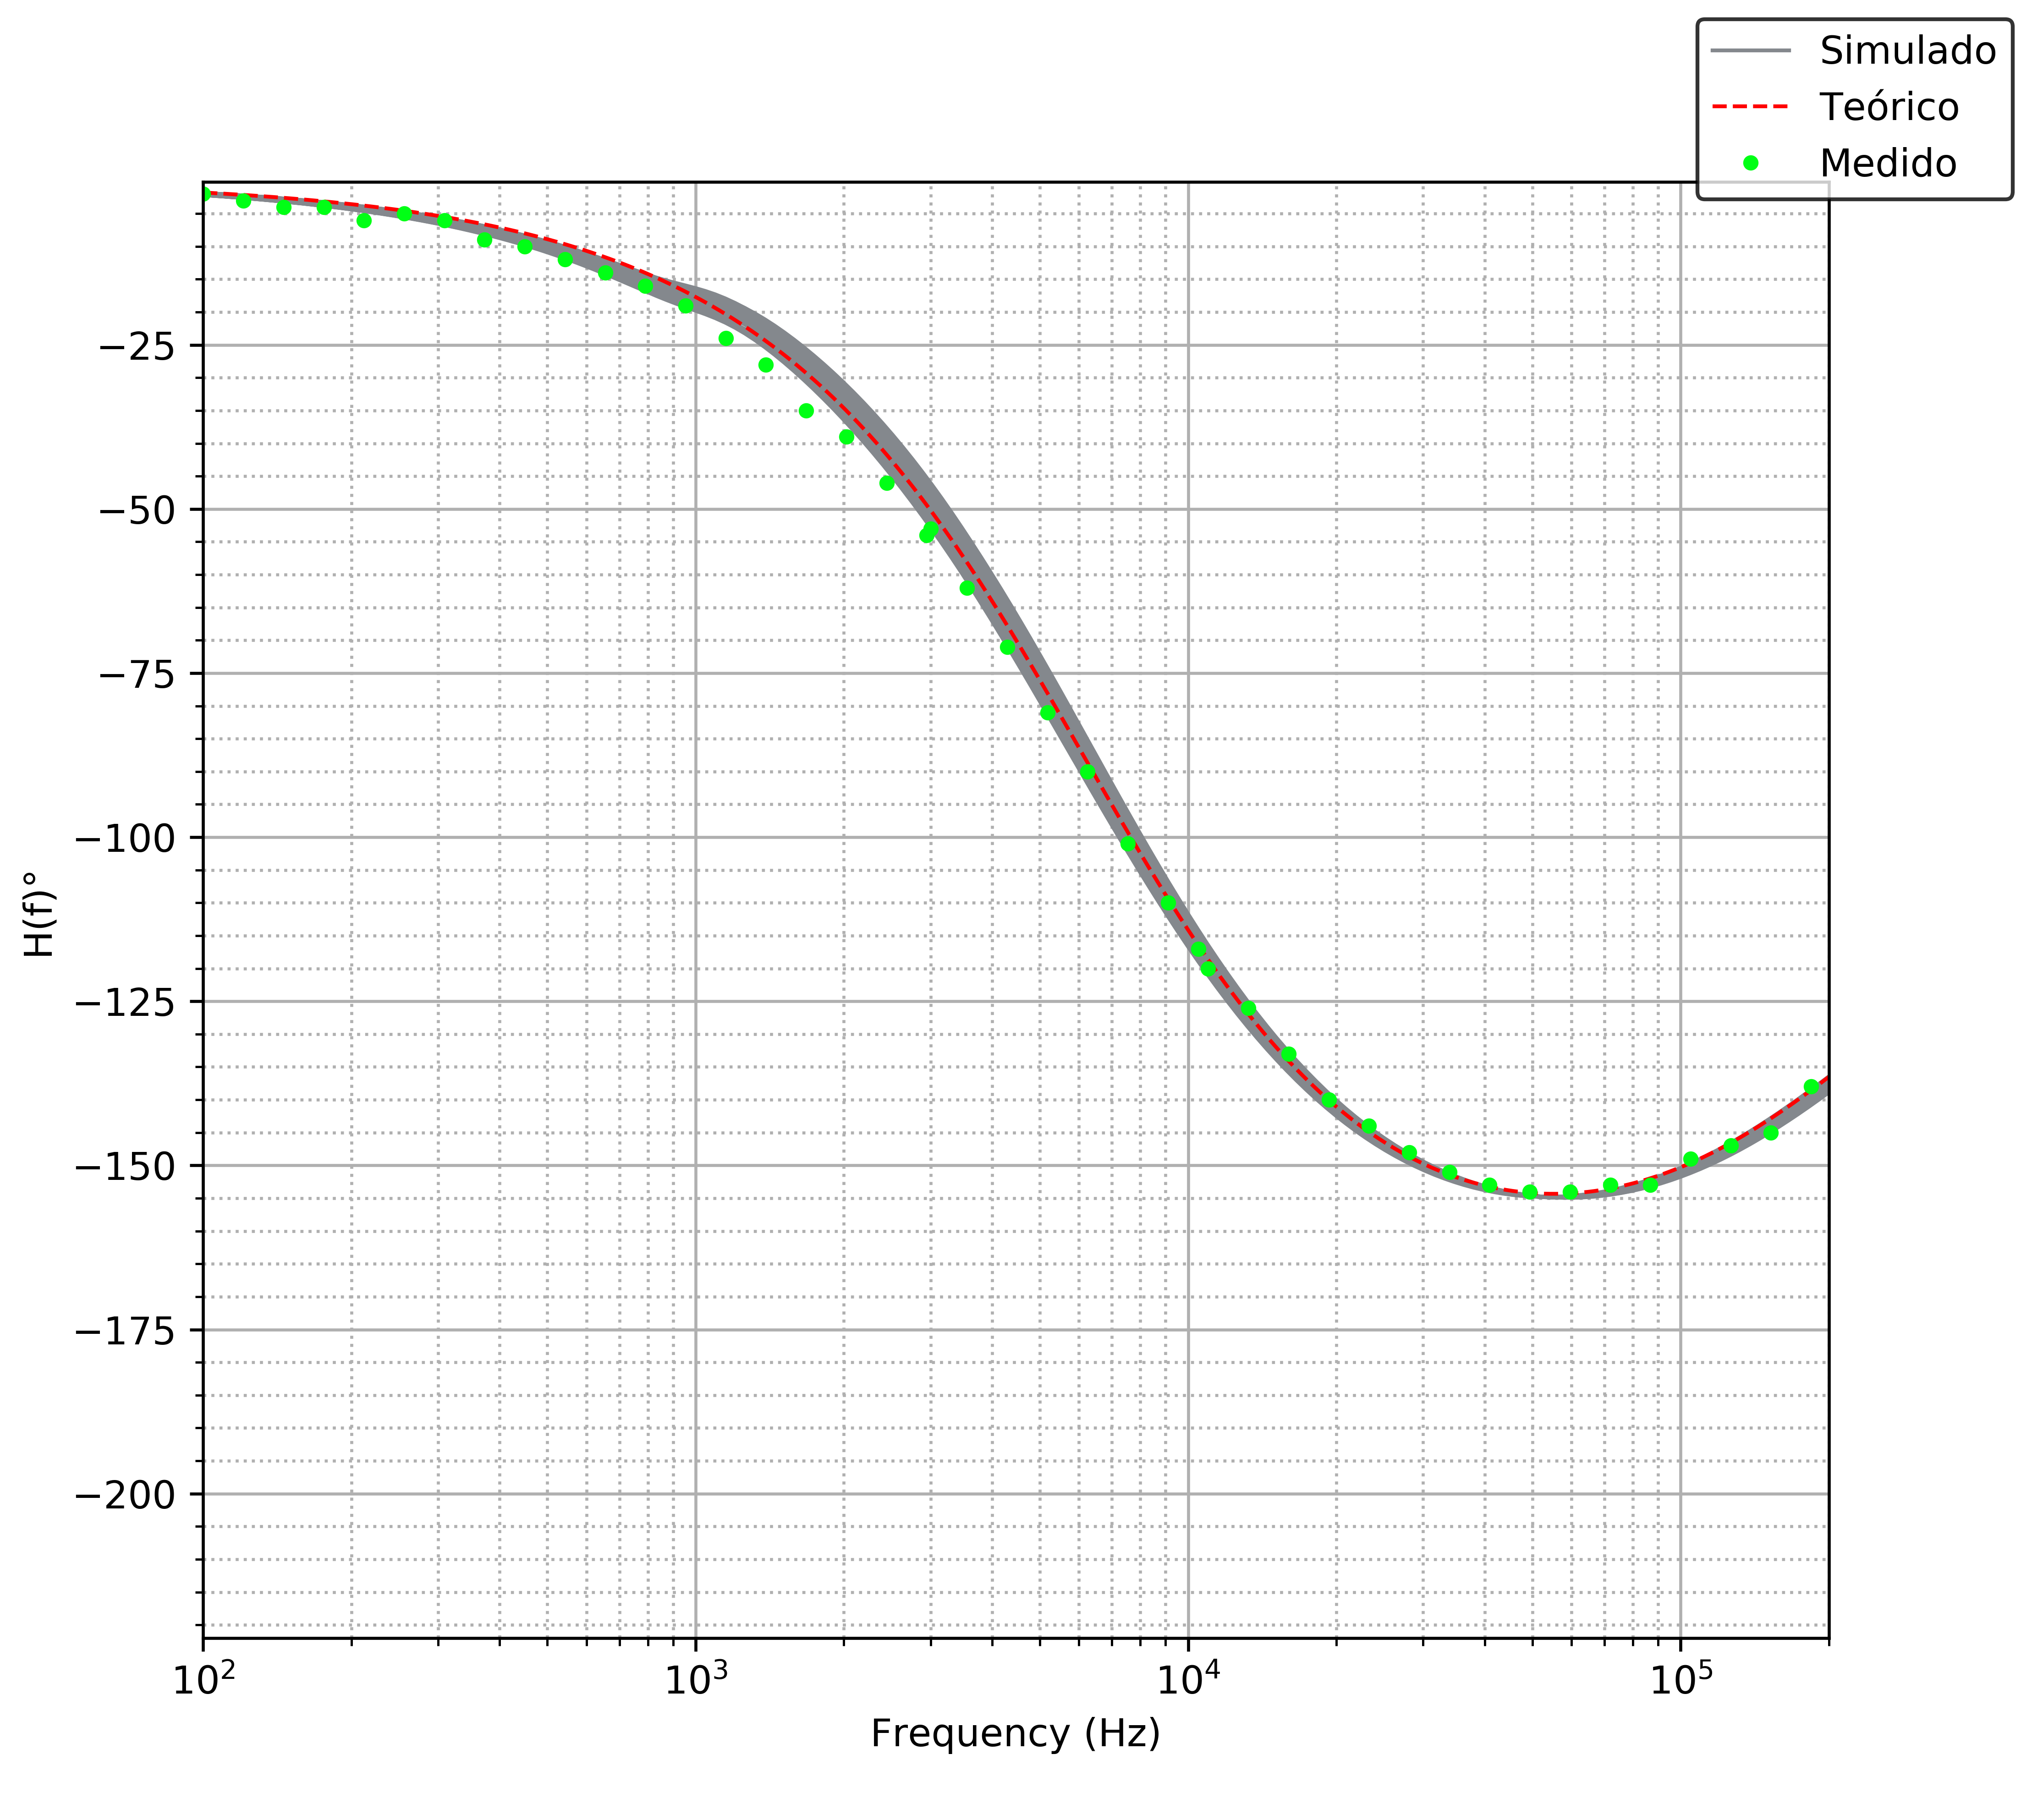
\includegraphics[scale=0.5]{../EJ2/Recursos/bode_pasabajos_fase.png}
    \caption{Diagrama de bode en fase del filtro pasabajos}
    \label{fig:bode_pasabajos_fase}
\end{figure}

\subsection{Filtro Pasaaltos}

\subsubsection{Dise\~no de funci\'on transferencia}
Consid\'erese un sistema de segundo orden lineal, de tiempo invariante y bibo-estable, tal que describe un comportamiento
pasaaltos, expresado por la Ec. \ref{eq:funcion_pasaaltos}.

\begin{equation}
    H(s) = \frac{ \frac{s^{2}}{\omega_o^{2}} }{\left(\frac{s}{\omega_o}\right)^{2} + s \cdot \frac{2 \cdot \xi}{\omega_o} + 1}
\end{equation}

La funci\'on transferencia caracteriza un sistema de segundo orden el cual se puede encontrar en tres diferentes condiciones, sea subamortiguado, sobreamortiguado o cr\'iticamente amortiguado,
para lo cual se descarta la primera posibilidad ya que provocar\'ia la aparici\'on de un sobrepico en el entorno de la frecuencia de corte, modificando la respuesta deseada. Por otro lado, se desea que el resultado
sea lo m\'as comparable con un filtro ideal, con lo cual para simular el cambio m\'as abrupto posible se busca que sea cr\'ticamente amortiguado para tener la mayor pendiente posible de decrecimiento, para el orden dado.
Esto \'ultimo implica que se condiciona al sistema a tener un valor de $\xi = 1$.

\begin{equation}
    H(s) = \frac{\left(\frac{s}{\omega_o}\right)^{2}}{\left(\frac{s}{\omega_o} + 1\right)^{2}}
    \label{eq:funcion_pasaaltos}
\end{equation}

Luego es necesario determinar la frecuencia de corte de dicho filtro. Para determinar este valor se toma como condici\'on de dise\~no cumplir con la plantilla presentada al inicio de la secci\'on, con lo cual
se eval\'ua la magnitud de la respuesta en frecuencia para las dos frecuencias de referencia y se imponen condiciones tomando un determinado margen de error.

\begin{eqnarray*}
    & |H(\omega_p)|dB > -2dB \Rightarrow 20 \cdot \log{\left( \frac{\frac{\omega_p^{2}}{\omega_o^{2}}}{1 + \frac{\omega_p^{2}}{\omega_o^{2}}} \right)} \\
    & \Rightarrow \omega_o < 2\pi \cdot 1.78kHz 
\end{eqnarray*}

\begin{eqnarray*}
    & |H(\omega_a)|dB < -11dB \Rightarrow 20 \cdot \log{ \left(  \frac{\frac{\omega_a^{2}}{\omega_o^{2}}}{1 + \frac{\omega_a^{2}}{\omega_o^{2}}} \right) } \\
    & \Rightarrow \omega_o > 2\pi \cdot 1.596kHz
\end{eqnarray*}

A partir de esto se puede considerar que siempre y cuando la frecuencia de corte que limite a quedar acotada dentro del rango $1.59kHz < f_o < 1.78kHz$ luego se cumplir\'an
las condiciones de dise\~no que fueron impuestas sobre el sistema. En caso de variar el valor de tal frecuencia, lo mejor es tomar como valor nominal el punto medio del rango, para tener la m\'axima
variaci\'on posible de forma sim\'etrico, con lo cual se escoge $f_o = 1.688kHz$. Con esta apreciaci\'on se puede ver que la variaci\'on de tal frecuencia que se permite es, porcentualmente,
un $5.4\%$.

\subsubsection{Dise\~no de circuito con Gyrator}

En un principio para poder implementar en un circuito un filtro pasaaltos descripto por la Ec. \ref{eq:funcion_pasaaltos} podr\'ia utilizarse una configuraci\'on RLC determinada,
con lo cual si se posee un Gyrator que ya de por s\'i corresponde equivalentemente a una inductor con una resistencia en serie, en principio se podr\'ia asumir que agregando un capacitor en serie ya es suficiente.
Esto fue lo que se intent\'o hacer con el circuito equivalente de la Fig. \ref{fig:equivalente_pasaaltos_fallido}.

\begin{figure}[H]
    \centering
    \includegraphics[scale=0.6]{../EJ2/Recursos/equivalente_pasaaltos_fallido.png}
    \caption{Circuito equivalente fallido}
    \label{fig:equivalente_pasaaltos_fallido}
\end{figure}

\begin{equation*}
    H(s) = \frac{s^{2} \cdot LC \cdot (1 + \frac{R_L}{s \cdot L})}{s^{2} \cdot LC + s \cdot C \cdot R_L + 1}
    \label{eq:funcion_pasaaltos_fallida}
\end{equation*}

El problema de este circuito o esta configuraci\'on propuesta se refleja en la Ec. \ref{eq:funcion_pasaaltos_fallida}, si se observa con atenci\'on difiere con respecto a la que idealmente se dise\~no por un factor
adicional en el numerador, esto se debe a la presencia de la resistencia $R_L$ en la rama de salida y lo que ser\'ia beneficioso a los fines de este an\'alisis ser\'ia poder despreciar el efecto de tal factor en la funci\'on, no obstante para ello
habr\'ia que plantear $\frac{R_L}{\omega \cdot L} << 1 \Rightarrow \frac{R_L}{L} << \omega$. Es ac\'a donde esta propuesta falla en el sentido en que su comportamiento se va a desviar mucho de lo buscado,
ya que ese t\'ermino muy dif\'ilmente cumpla tal condici\'on, y se puede ver si se plantean las condiciones sobre $R_L$ y $L$ para cumplir inicialmente con el valor de $\xi$ y de $\omega_o$ del sistema.

\begin{align*}
    & L = \frac{1}{(2 \pi \cdot f_o)^{2} \cdot C} \\
    & R_L = \frac{1}{\pi \cdot f_o \cdot C} \\
    & \Rightarrow \frac{R_L}{L} = 4 \pi \cdot f_o
\end{align*}

Esto quiere decir que para las frecuencias de inter\'es, ya sean las de referencia para el filtro o la de corte, el factor tendr\'a un efecto apreciable que modificar\'a
su comportamiento resultante. 

\paragraph*{Circuito equivalente aproximado:} Para solucionar esto, se propone una nueva forma del circuito, agregando una resistencia en serie al capacitor como se puede observar en la Fig. \ref{fig:equivalente_pasaaltos}.

\begin{figure}[H]
    \centering
    \includegraphics[scale=0.6]{../EJ2/Recursos/equivalente_pasaaltos.png}
    \caption{Circuito equivalente del filtro pasaaltos}
    \label{fig:equivalente_pasaaltos}
\end{figure}

En primer lugar, si bien el sistema a analizar es el que comienza posterior a la resistencia del generador, es importante tener en cuenta su valor y buscar que la resistencia
$R$ sea mucho m\'as grande para que las desviaciones al sistema por la presencia de $R_G$ sean m\'inimas, es decir, que se cumpla que $R_G << R$. De esta forma la resistencia total
del circuito RLC no se desviar\'a mucho del valor esperado para el caso amortiguado que se busca. Con esto en mente, se desarrolla y se llega a que la funci\'on transferencia est\'a dada:

\begin{align}
    & H(s) = \frac{s^{2} \cdot LC \cdot (1 + \frac{R_L}{s \cdot L})}{1 + s \cdot C \cdot (R_L + R) + s^{2} \cdot LC} \\
    & \xi = 1 \Rightarrow R + R_L = \frac{1}{\pi \cdot f_o \cdot C} = \frac{1}{\pi \cdot 1.688kHz \cdot C}\\
    & L = \frac{1}{(2 \pi \cdot f_o)^{2} \cdot C} = \frac{1}{(2 \pi \cdot 1.688kHz)^{2} \cdot C}
\end{align}

Nuevamente en este circuito se puede ver que hay un factor en el numerador que en la expresi\'on ideal no se encuentra, con lo cual se busca despreciar sus efectos. Para lograr esto, y de la misma forma que se analiz\'o en el caso del circuito fallido,
se debe imponer que se cumpla que $\frac{R_L}{L} << \omega$. Esta vez esto es posible, el por qu\'e se atribuye a que la presencia de una nueva resistencia en el circuito influye en el valor del coeficiente de amortiguamiento con lo cual no est\'a determinado
el valor de $R_L$ y este nuevo grado de libertad permite dividir los requisitos entre las resistencias. Se propone considerar que la frecuencia por debajo de la cual deberia volverse apreciable tal factor est\'e debajo de $f \approx 100Hz$ por considerar una d\'ecada
de separaci\'on con la primer frecuencia de referencia y evitar las desviaciones pertinentes. Entonces adem\'as se impone $R_L << 2\pi \cdot 100Hz \cdot L$.

Se propone un valor de capacidad $C = 33nF$, con lo cual la inductancia tiene que tener un valor de $L = 269.39mH$. Consecuentemente, la resistencia $R_L < 169.26 \Omega$, y luego la suma de ambas resistencia
tiene un valor de $R + R_L = 5714.3 \Omega$, por lo cual se toma $R_L = 120 \Omega$ y $R = 5.6k\Omega$. Si se tiene en cuenta que para la implementaci\'on pr\'actica de estos circuitos se utilizar\'an resistencia SMD
de potencia nominal 1/8W, resulta necesaria hacer una menci\'on sobre el valor bajo de $R_L$ y analizar la posibilidad de que implica una potencia disipada mayor. No obstante, como esta resistencia en el circuito equivalente se encuentre en la rama de 
salida en serie con la inductancia, para las frecuencias bajas en las cuales tal resistencia sea comparable con la magnitud de la impedancia del inductor, luego la salida se ver\'a atenuada demasiado como para producir una ca\'ida de tensi\'on que genere disipaci\'on
por encima de lo nominal, por otro lado, en las condiciones en las cuales la salida no se ve atenuada luego la impedancia del inductor crece en magnitud y la proporci\'on sobre la resistencia disminuye, con lo cual al igual que antes tampoco puede producir una disipaci\'on notable.

\paragraph*{Circuito completo:} En la Fig. \ref{fig:circuito_pasaaltos} se puede observar el esquema completo del circuito implementando la bobina, es decir el inductor con una resistencia en serie, empleando para ello un Gyrator.
Es necesario por ende determinar los valores del circuito para que simule efectivamente al inductor, para lo cual se parte inicialmente de una condici\'on, donde se pide que $\frac{1}{C_2 \cdot R_L} > 2 \pi \cdot 500kHz$. Esto \'ultimo es para alejar los efectos no deseados del Gyrator, despreciandolos
y considerando que para frecuencias bajas del filtro luego se comporte como inductor, no obstante el valor dado de frecuencia es una elecci\'on arbitraria. Por otro lado, a partir de tal consideraci\'on se propone $C_2 = 2.7nF$ y se obtiene que como $L = R_L \cdot C_2 \cdot R_2$, entonces $R_2 = 820k\Omega$.

\begin{figure}[H]
    \centering
    \includegraphics[scale=0.55]{../EJ2/Recursos/circuito_pasaaltos.png}
    \caption{Circuito completo del pasaaltos}
    \label{fig:circuito_pasaaltos}
\end{figure}

\paragraph*{An\'alisis no ideal:} Si se considera un amplificador operacional no ideal, esto es, con un $A_{vol}$ finito y con polo dominante, luego adem\'as
se considera que la corriente de entrada es despreciable, entonces planteando diferentes ecuaciones para caracterizar al circuito se puede llegar a la funci\'on transferencia
del mismo.

\begin{align}
    & V_p = \frac{V_o \cdot R_2}{R_2 + \frac{1}{s \cdot C_2}} \\
    & A_{vol} = \frac{GBP}{s + \omega_p} \\
    & V_n = (V_p - V_n) \cdot A_{vol} \\
    & \frac{V_i - V_o}{R + \frac{1}{s \cdot C}} = \frac{V_o}{R_2 + \frac{1}{s \cdot C_2}} + \frac{V_o - V_n}{R_L}
\end{align}

\begin{align*}
    & a = \frac{C_2 \cdot R_2}{GBP + \omega_p}\\
    & b = C_2 \cdot R_2 \cdot (1 + \frac{1}{C_2 \cdot R_2 \cdot(GBP + \omega_p)})\\
    & \alpha = C \cdot C_2 \cdot \frac{R \cdot R_2 + R \cdot R_L + R_2 \cdot R_L}{GBP + \omega_p}\\
    & \beta = \frac{ C \cdot C_2 \cdot R_L \cdot GBP \cdot (R + R_2) + C \cdot C_2 \cdot \omega_p \cdot (R \cdot R_2 + R \cdot R_L + R_2 \cdot R_L) + C \cdot (R + R_L) + C_2 \cdot (R_2 + R_L)}{GBP + \omega_p} \\
    & \gamma = \frac{C \cdot (GBP + \omega_p) \cdot (R + R_L) + C_2 \cdot (GBP \cdot R_L + \omega_p \cdot (R_2 + R_L)) }{GBP + \omega_p}\\
    & H(s) = \frac{s \cdot C \cdot R_L \cdot \left[s^{2} \cdot a + s \cdot b + 1 \right]}
    {\alpha \cdot s^{3} + \beta \cdot s^{2} + \gamma \cdot s + 1}
\end{align*}

Considerando que $GBP >> \omega_p$, luego si se considera que $\omega << \frac{1}{C_2 \cdot R_2 \cdot(GBP + \omega_p)}$ entonces el numerador de la expresi\'on se puede reducir
a considerar que $Num[H(s)] \approx s^{2} \cdot C \cdot C_2 \cdot R_2 \cdot R_L$. Por otro lado si se estima que $R_L < R < R_2$, entonces despreciando una con respecto a la otra dentro de la funci\'on,
y considerando que $\frac{GBP}{GBP + \omega_p} \approx 1$ se puede reducir la expresi\'on del t\'ermino cuadr\'atico. Luego el factor c\'ubico del denominador puede ser despreciado para las frecuencias de operacion
ya que $\omega^{3} << \frac{GBP}{C \cdot C_2 \cdot R \cdot R_2}$ en las frecuencias de operaci\'on. Finalmente, el t\'ermino lineal del denominador se puede reducir aplicando las aproximaciones ya tomadas, entonces se obtiene:

\begin{equation}
    H(s) = \frac{s^{2} \cdot C \cdot C_2 \cdot R_L \cdot R_2}{s^{2} \cdot C \cdot C_2 \cdot R_2 \cdot R_L + s \cdot C \cdot (R + R_L) + 1}
\end{equation}
 
\subsubsection{Verificaci\'on del dise\~no}
Se verifica a continuaci\'on el funcionamiento del dise\~no del filtro empleando una herramiento de simulaci\'on LTSpice y graficando usando Monte Carlo para considerar las variaciones
por la dispersi\'on de los componentes. Los resultados son ilustrados en las figuras \ref{fig:hp_montecarlo} y \ref{fig:hp_montecarlo_frecuencias}.

\begin{figure}[H]
    \centering
        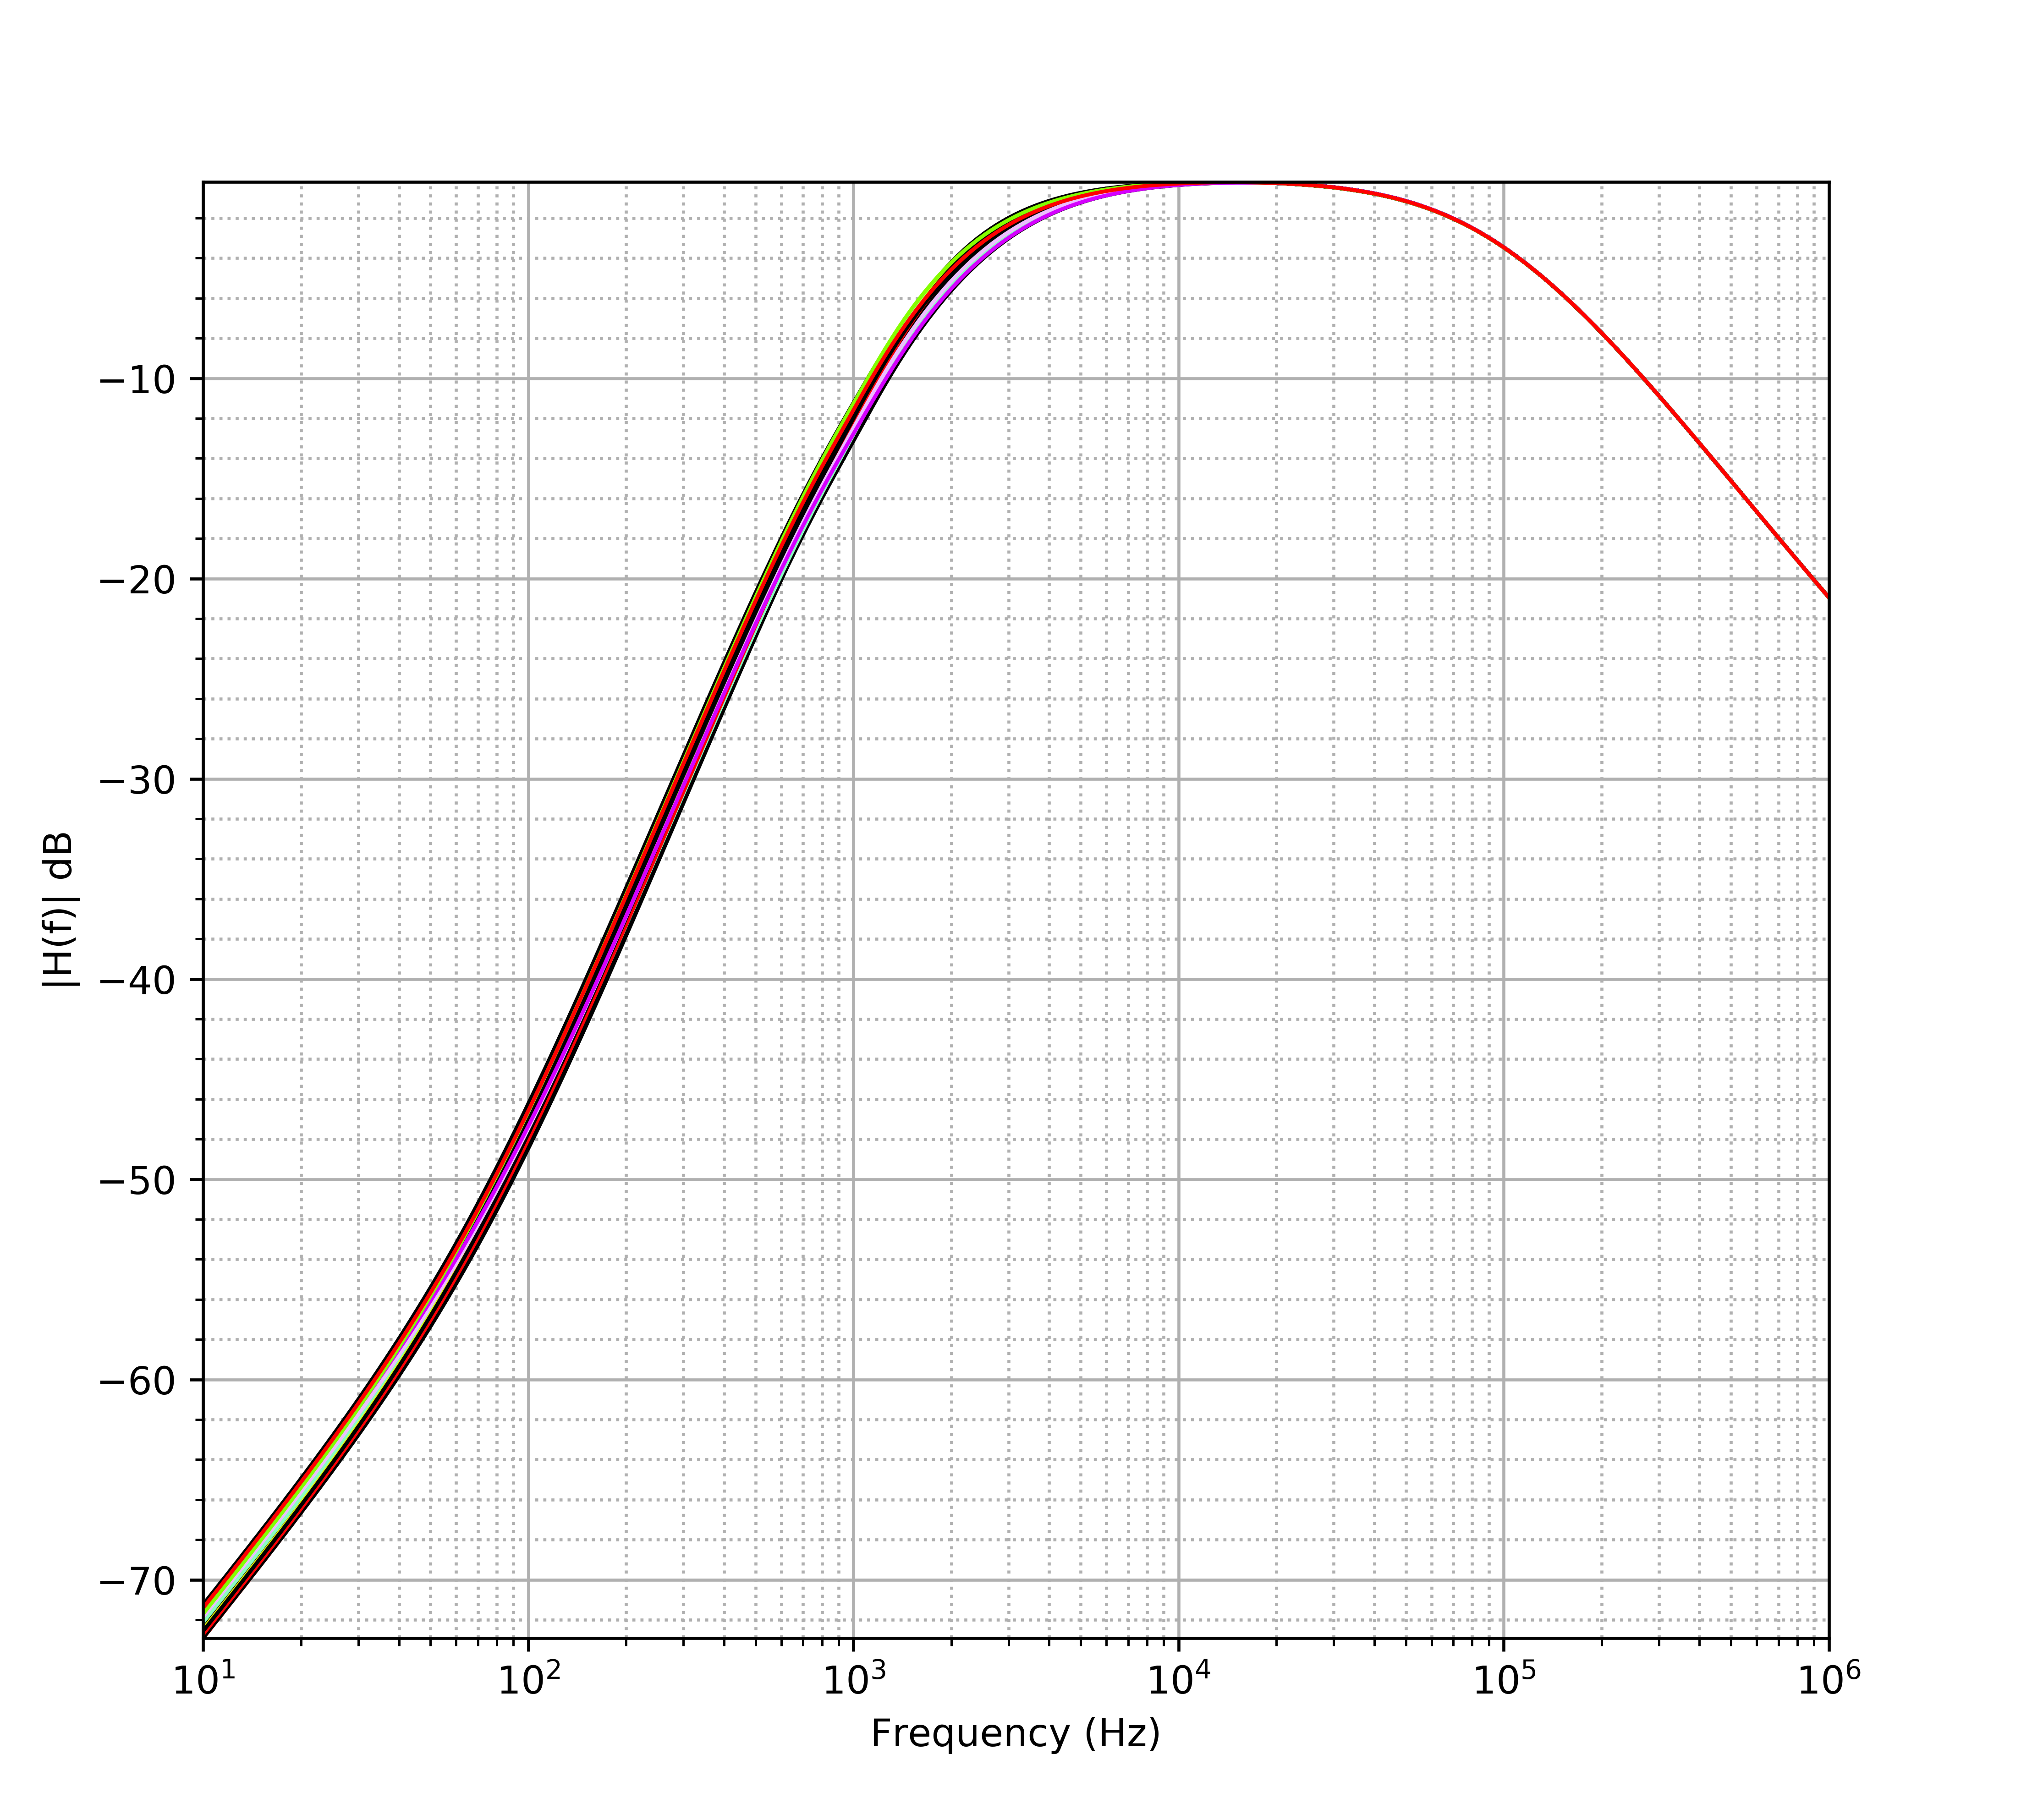
\includegraphics[scale=0.12]{../EJ2/Recursos/hp_montecarlo.png}
    \caption{Respuesta en frecuencia en m\'odulo del filtro pasaaltos}
    \label{fig:hp_montecarlo}
\end{figure}

\begin{figure}[H]
    \centering
    \begin{tabular}{c c}
        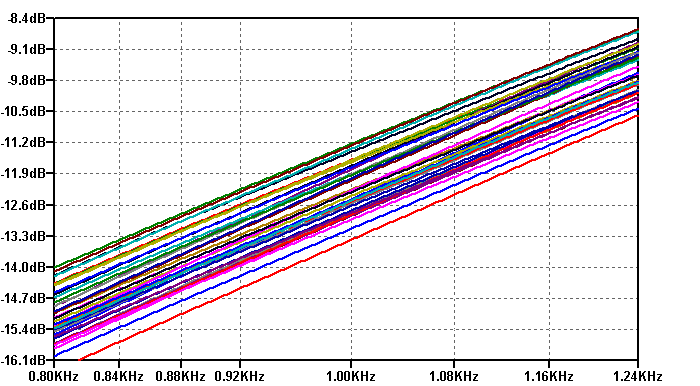
\includegraphics[scale=0.4]{../EJ2/Recursos/hp_montecarlo_fa.png}
        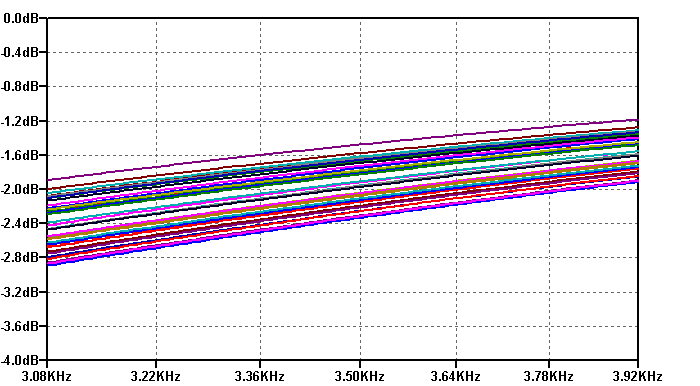
\includegraphics[scale=0.4]{../EJ2/Recursos/hp_montecarlo_fp.png}
    \end{tabular}
    \caption{Acercamiento en frecuencias pasante y atenunante}
    \label{fig:hp_montecarlo_frecuencias}
\end{figure}

\subsubsection{Resultados}
En las Fig. \ref{fig:bode_pasaaltos_modulo} y \ref{fig:bode_pasaaltos_fase} se pueden observar los resultados constrastados del an\'alisis te\'orico, la simulaci\'on y las mediciones de la implementaci\'on pr\'actica.

Para la $f = 1kHz$ se midi\'o $|H(f)| = -11.6dB$ y una fase de $108^{\circ}$.
Para la $f = 3.5kHz$ se midi\'o $|H(f)| = -2.5dB$ y una fase de $44^{\circ}$.

La respuesta en frecuencia observada para frecuencias menores a $f \approx 50kHz$ corresponde efectivamente
a un filtro pasaaltos, no obstante para frecuencias mayores ya se puede observar un decaimiento de la misma que se produce
porque el circuito Gyrator deja de comportarse como un inductor por las razones ya fundamentadas previamente en los an\'alisis te\'oricos.

\begin{figure}[H]
    \centering
        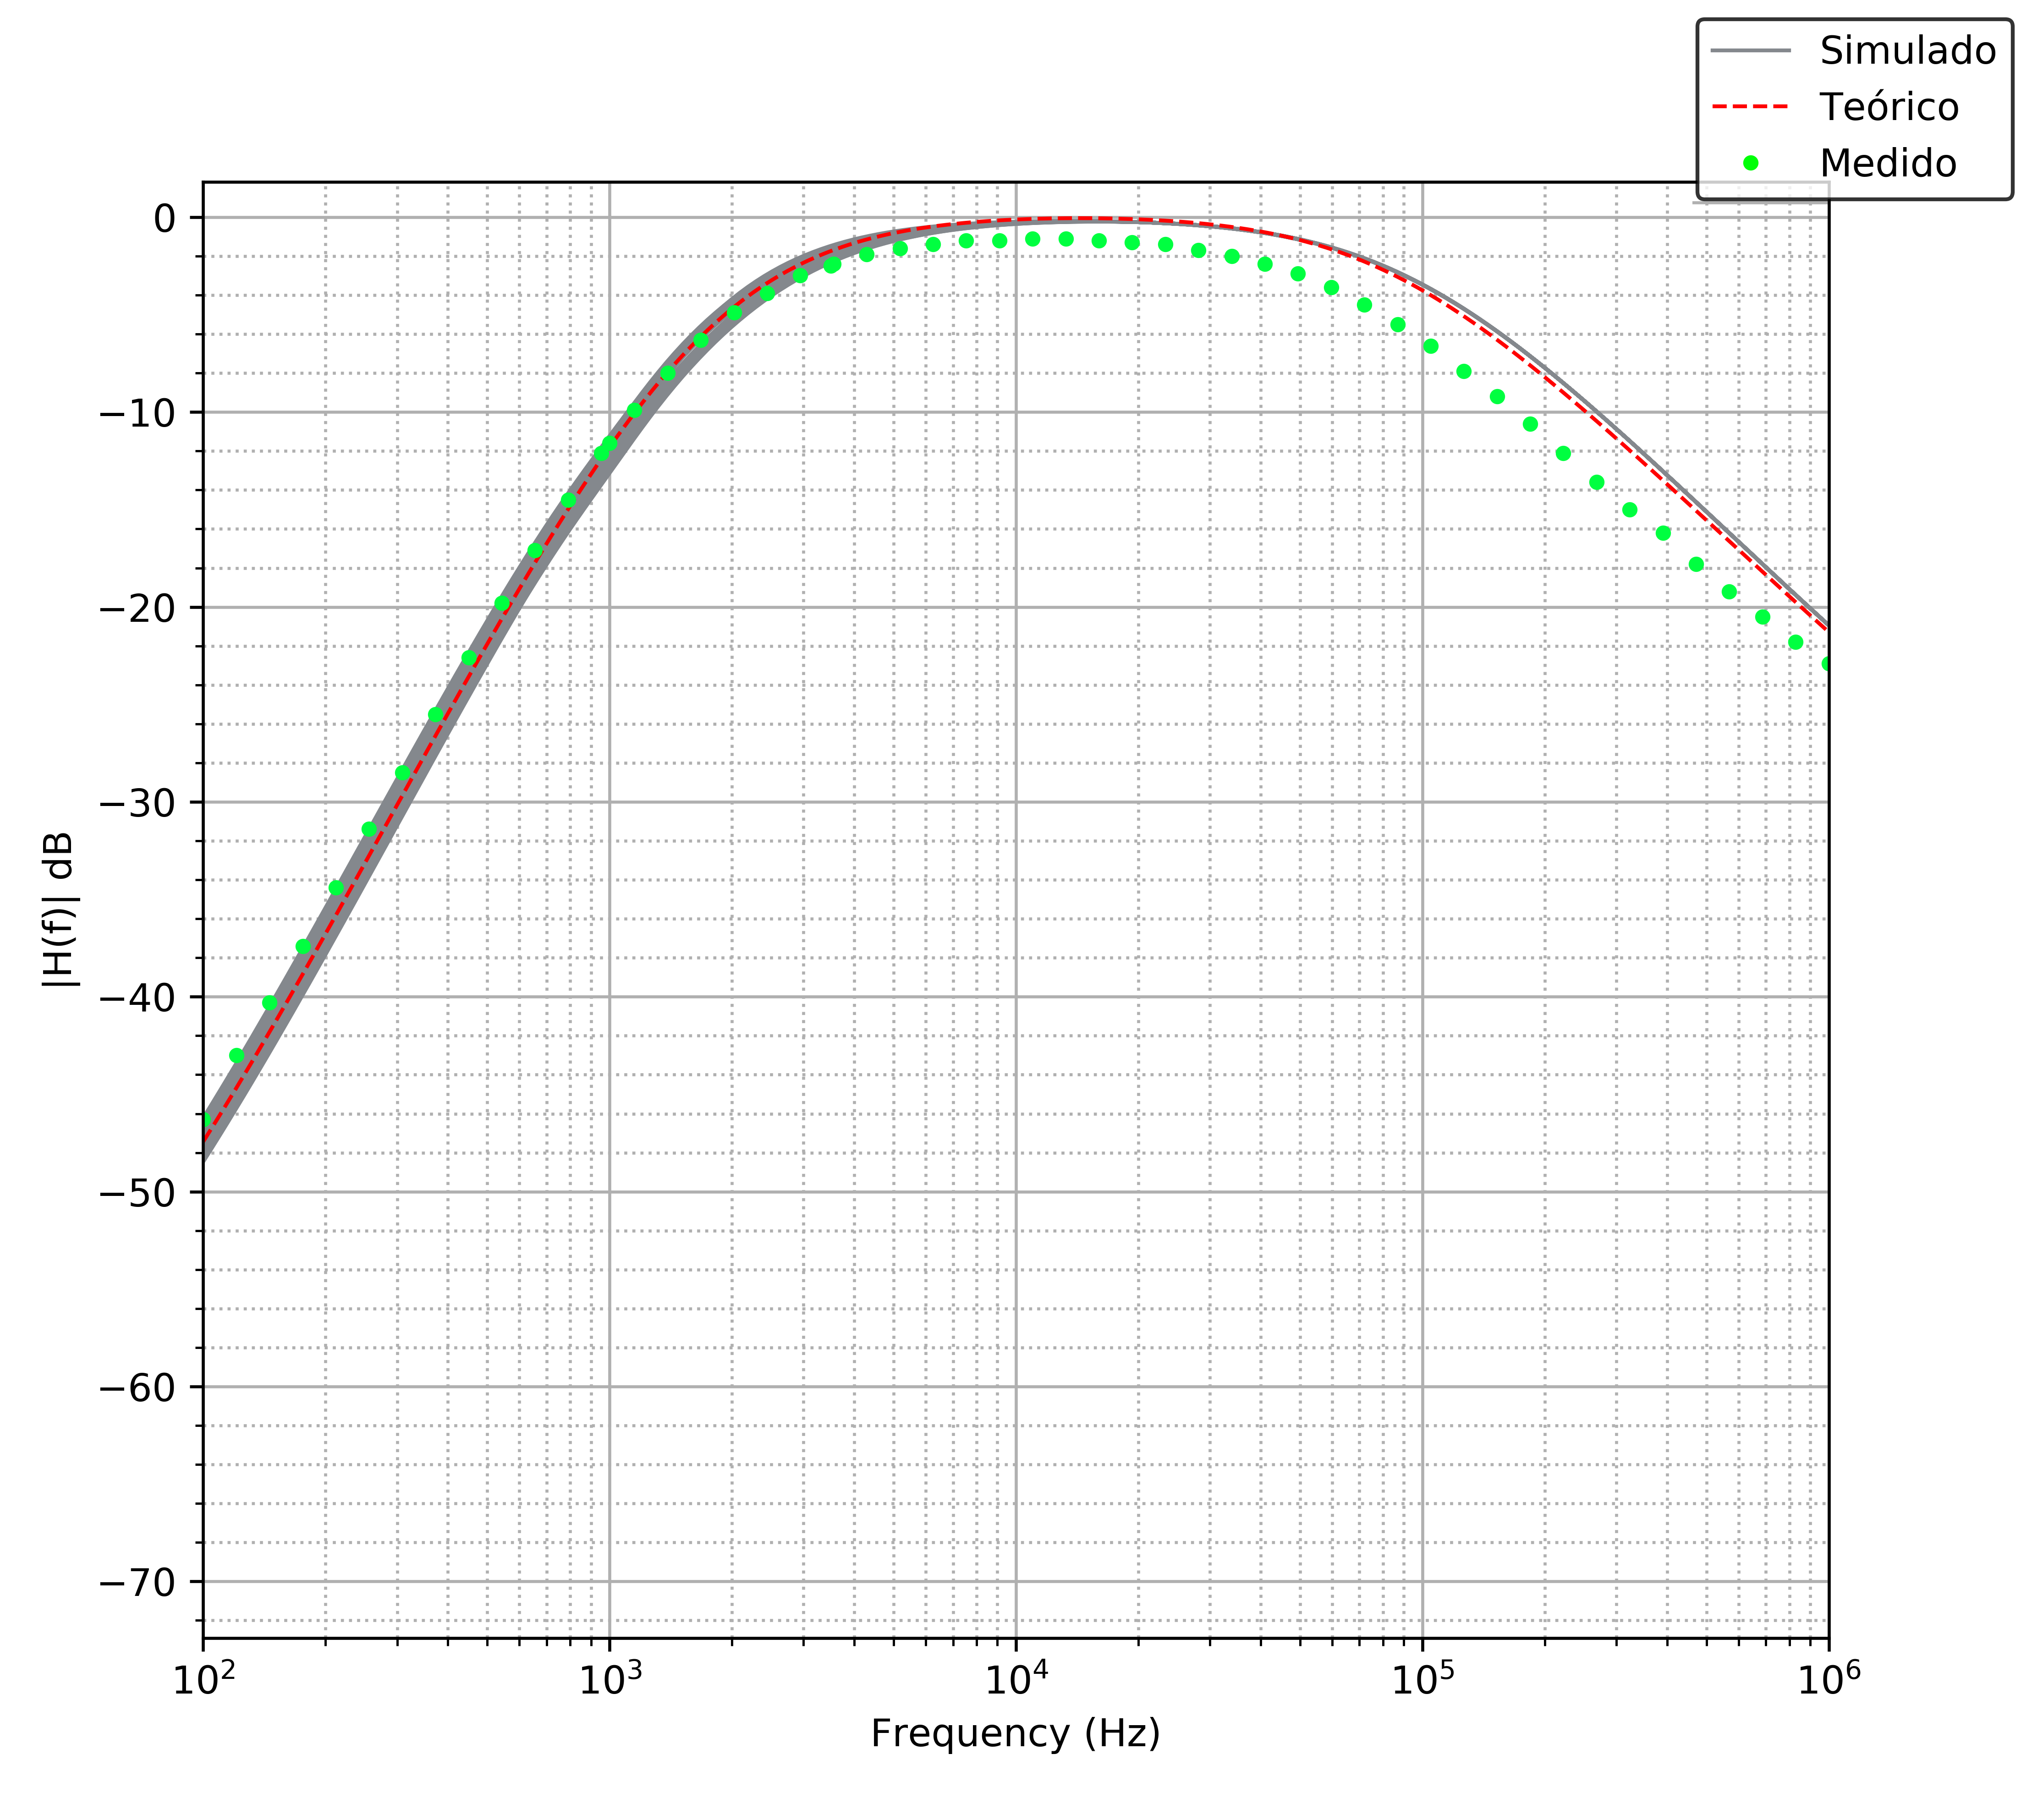
\includegraphics[scale=0.1]{../EJ2/Recursos/bode_pasaaltos_modulo.png}
    \caption{Diagrama de bode en m\'odulo del filtro Pasaaltos}
    \label{fig:bode_pasaaltos_modulo}
\end{figure}

\begin{figure}[H]
    \centering
        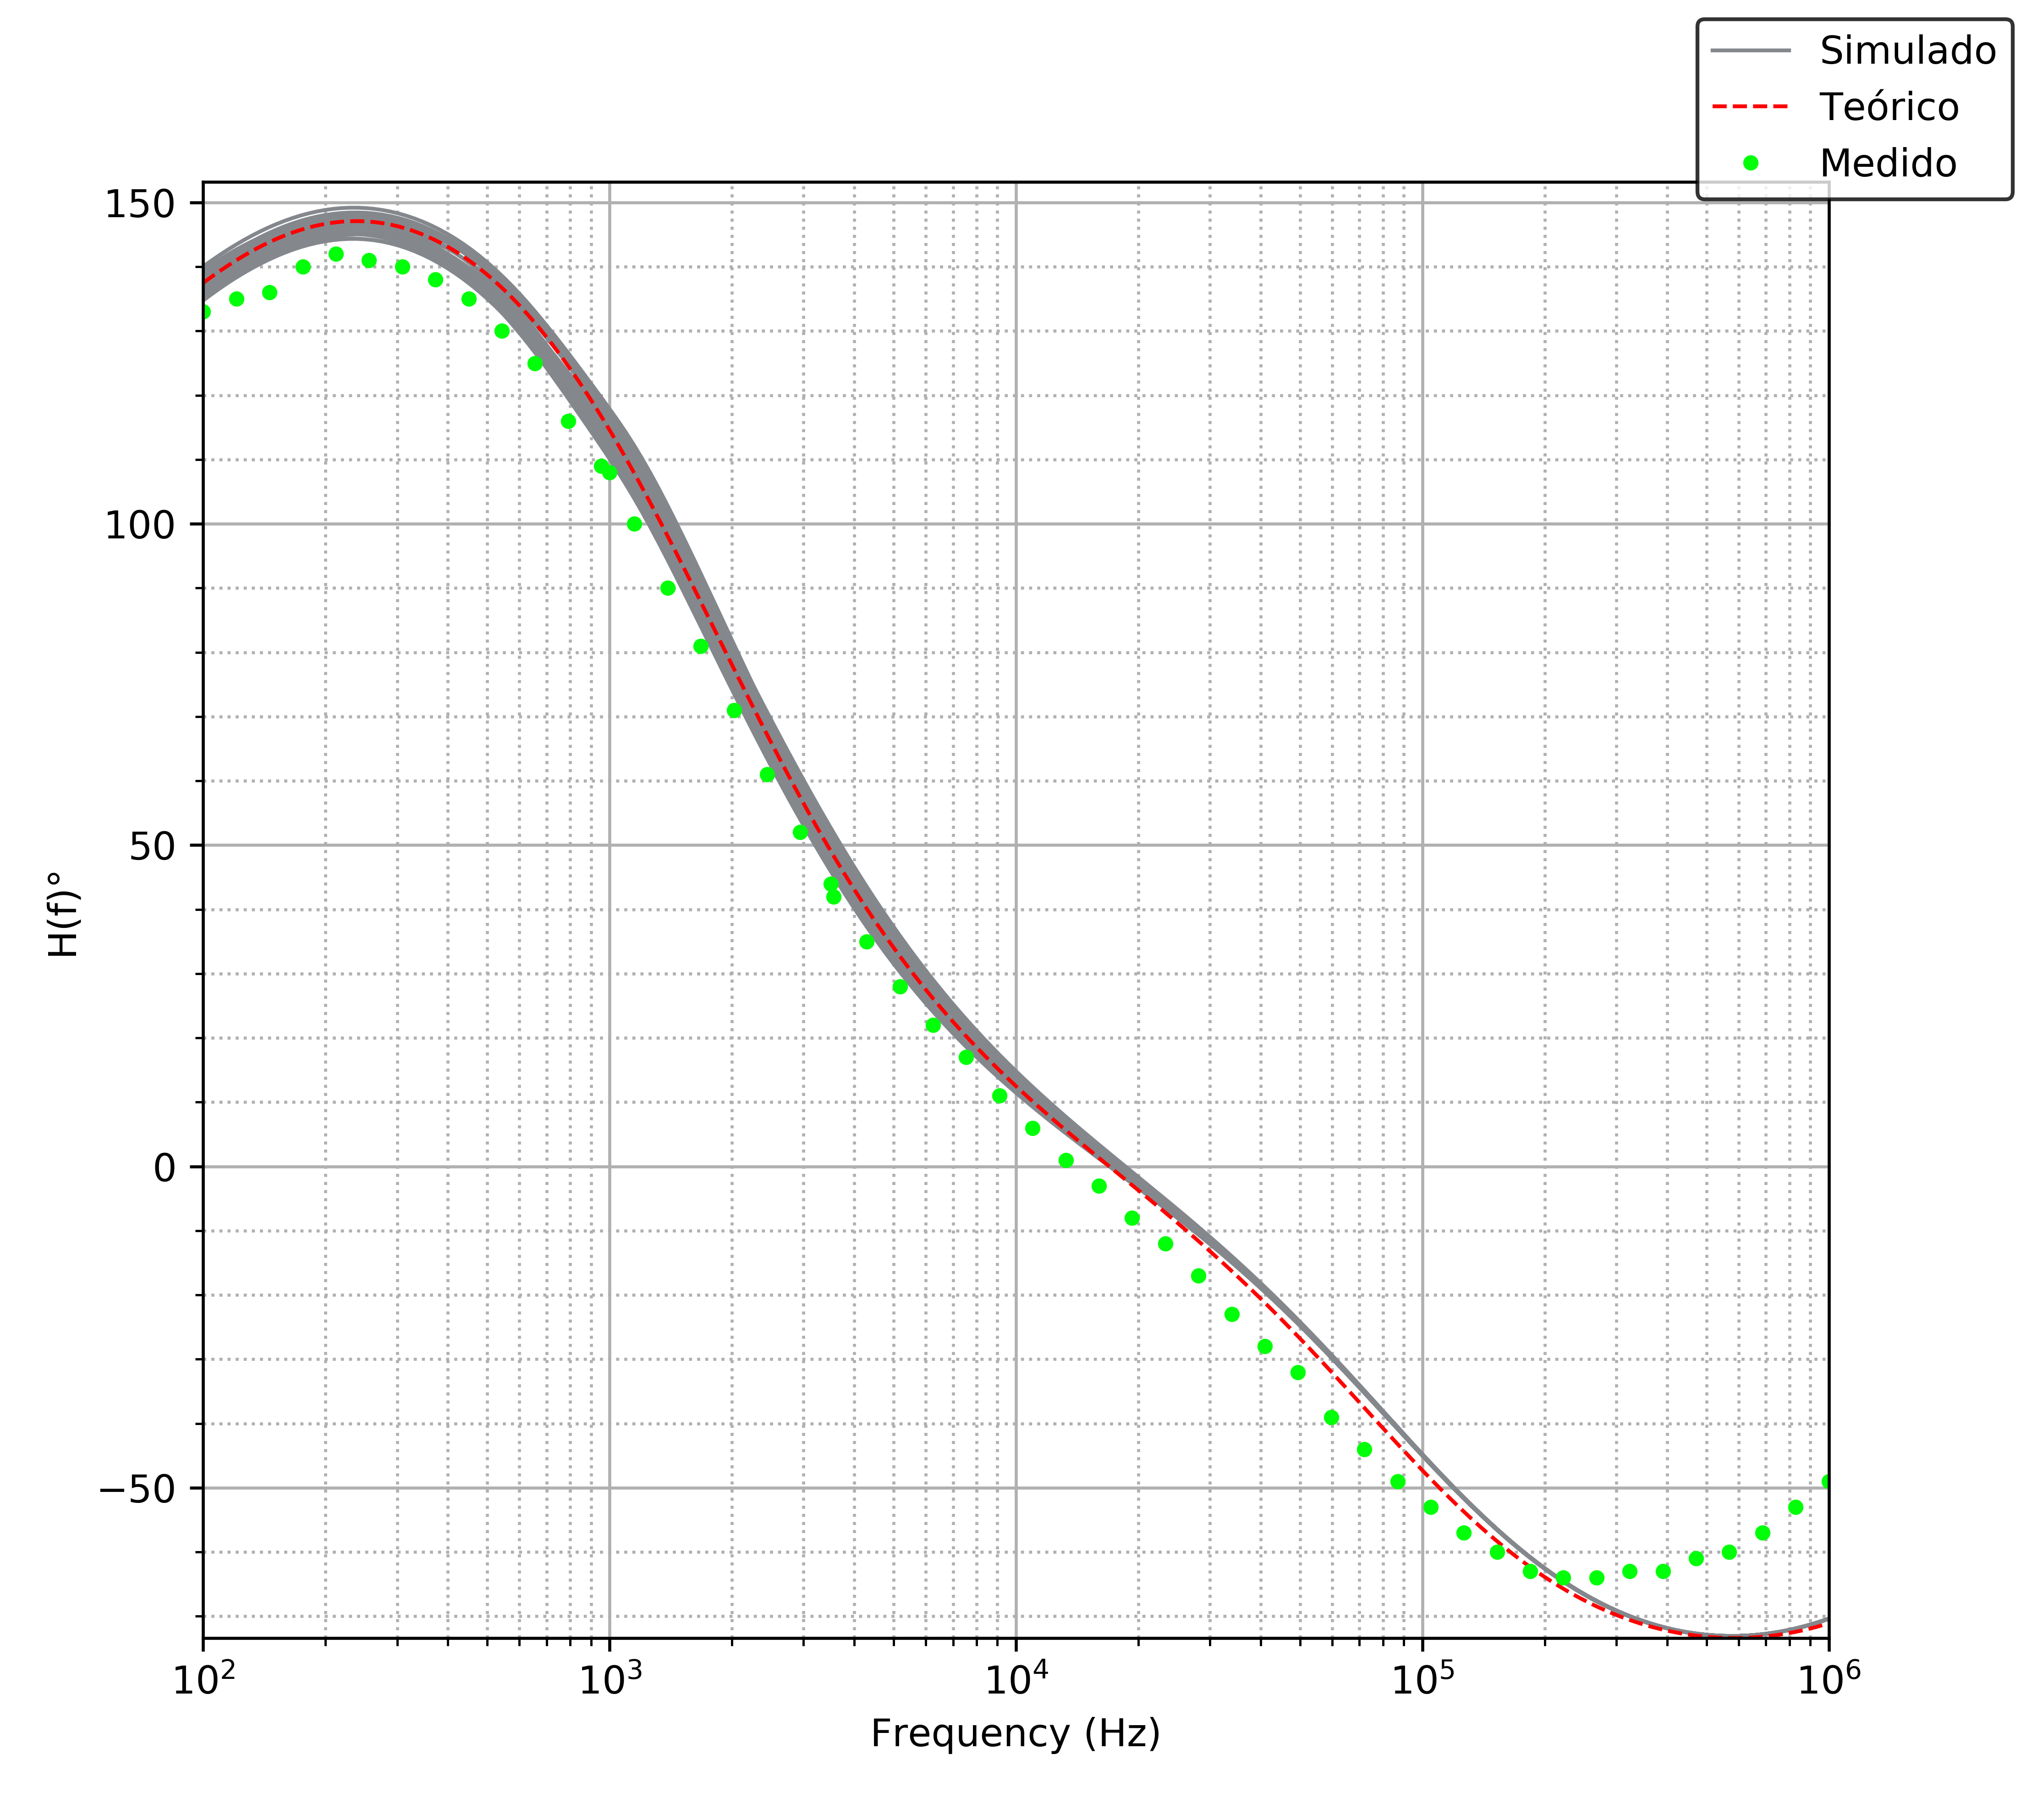
\includegraphics[scale=0.5]{../EJ2/Recursos/bode_pasaaltos_fase.png}
    \caption{Diagrama de bode en fase del filtro Pasaaltos}
    \label{fig:bode_pasaaltos_fase}
\end{figure}

\subsection{Filtro Pasabanda}
\subsubsection{Dise\~no de funci\'on transferencia}
Consid\'erese un sistema de segundo orden lineal, de tiempo invariante y bibo-estable, el cual describe una respuesta en frecuencia caracter\'istica 
de un sistema pasabanda con la funci\'on de la Ec. \ref{eq:funcion_pasabanda}. Se define una constante arbitraria K que depender\'a posteriormente de la implementaci\'on del sistema.

\begin{equation}
    H(s) = \frac{s \cdot K}{\left( \frac{s}{\omega_o} \right)^{2} + \frac{S}{Q \cdot \omega_o} + 1}    
    \label{eq:funcion_pasabanda}
\end{equation}

Espec\'ificamente esta funci\'on transferencia debe atenuar todas aquellas frecuencias fuera del entorno de la $f_o = 6kHz$ seg\'un fue consignado como requisito del filtro, pero adem\'as se impone sobre el circuito
que como pasabanda debe tener un ancho de banda peque\~no que reduzca la extensi\'on del mencionado entorno, para lo cual se busca que el sistema se encuentre subamortiguado. Esto \'ultimo implica que la respuesta en frecuencia poseer\'a
un sobrepico que deber\'a ser ubicado en la frecuencia a filtrar y debe tenerse como cuidado o precauci\'on que no supere los $0dB$. Para lograr ello, se deriva y localiza el extremo absoluto de la funci\'on $|H(w)|$.

\begin{align*}
    & \frac{\delta |H(w)|}{\delta \omega} = 0 \Leftrightarrow \\
    & K \cdot \left[ (\omega_o^{2} - \omega^{2})^{2} + (\frac{\omega_o \cdot \omega}{Q})^{2} \right]
    = \frac{K \cdot \omega}{2} \cdot \left[ -4 \omega \cdot ( \omega_o^{2} - \omega^{2}) + \frac{\omega_o^{2} \cdot \omega \cdot 2}{Q} \right] \Leftrightarrow \\
    & \omega = \omega_o \\
    & |H(\omega_o)| = K \cdot Q \cdot \omega_o
\end{align*}

Por lo tanto, se impondr\'a al sistema que modelice esta expresi\'on matem\'atica, que el valor de $\omega_o = 2\pi \cdot 6kHz$ para cumplir con la frecuencia deseada, y adem\'as,
que cumpla con que $|H(\omega_o)| = K \cdot Q \cdot \omega_o \leq 0dB$.

\subsubsection{Dise\~no de circuito con Gyrator}
De igual forma que para los filtros ya dise\~nados previamente, se seguir\'a un proceso en el cual se dimensarionar\'an los componentes empleandos modelos ideales o aproximados,
determinando los criterios y condiciones donde se logren validar tales comportamientos. No obstante, en el caso de este filtro pasabanda y al igual que puede suceder con muchos circuitos,
existen diferentes alternativas sobre c\'omo implementarlo. Una de las particularidades que tiene este filtro a comparaci\'on del resto es que por filtrar un rango acotado y espec\'ifico de frecuencias,
luego la topolog\'ia del circuito influir\'a mucho sobre la capacidad de establecer con el menor error posible tales frecuencias, por esto mismo es que ante la presencia de dos alternativas, se estudian ambas
evaluando cu\'al de ellas puede llevar consigo mayores ventajas o beneficios.

\paragraph*{Circuito equivalente aproximado:} En un principio se analiza desde un punto de vista aproximado la funci\'on transferencia de ambos circuitos propuestos. El objetivo es comparar ambos comportamientos,
considerar las implicancias, y luego tener en cuenta otros aspectos para determinar la topolog\'ia m\'as conveniente.

\begin{figure}[H]
    \centering
    \begin{tabular}{c c}
        \includegraphics[scale=0.4]{../EJ2/Recursos/equivalente_pasabanda_alternativo.png} & 
        \includegraphics[scale=0.4]{../EJ2/Recursos/equivalente_pasabanda.png}
    \end{tabular}
    \caption{Equivalentes aproximados para el pasabanda, dos alternativas}
    \label{fig:equivalentes_pasabanda}
\end{figure}

Se referir\'a a cada circuito seg\'un el tipo de salida que poseen, por ser una salida con una rama LC o con una rama R, simplemente para facilitar el an\'alisis y las referencias. De esta forma,
en un principio se obtiene la expresi\'on de la funci\'on transferencia para el circuito con salida LC.

\begin{equation}
    H(s) = \frac{s \cdot L + R_L}{s^{2} \cdot L \cdot C \cdot R + s \cdot (C \cdot R \cdot R_L + L) + (R + R_L)}
\end{equation}

Luego para el caso del circuito de salida R.

\begin{equation}
    H(s) = \frac{s \cdot C \cdot R}{s^{2} \cdot L \cdot C + s \cdot C \cdot (R+ R_L) + 1}
\end{equation}

Ambos circuitos poseen una funci\'on transferencia que correctamente configurada puede ser empleada para definir un pasabanda, no obstante en primer lugar para bajas frecuencias el comportamiento es mejor en el circuito de salida R,
ya que en el de salida LC para frecuencias muy bajas la ganancia se mantiene casi constante, aunque podr\'ia ser definida baja y considerarse tal banda atenuada. Esto resulta observable directamente del hecho que la funci\'on $H(s)$ de la salida R
tiene la forma m\'as parecida con el modelo matem\'atico propuesto, ya que posee un cero en el cero.

Por otro lado, en ambos circuitos tanto la inductancia como la capacitancia definen parcialmente la frecuencia de corte, pero en el primer caso de la salida LC adem\'as los valores de las resistencias tambi\'en influyen,
lo cual puede no ser deseado desde dos puntos de vista. En primer lugar, desde un an\'alisis f\'isico, se esperar\'ia que la resonancia de una red compuesta por componentes LC est\'e \'unicamente definida por ellos, variando seg\'un las resistencias
el car\'acter de amortiguamiento. Por otro lado, al haber m\'as componentes que definen una misma variable esto puede implicar que es m\'as sensible en t\'erminos generales a variaciones de todos los componentes.

Finalmente, otro aspecto a comparar es la modulaci\'on de fase que producen a las se\~nales seg\'un la frecuencia estos circuitos. Mientras que el circuito de salida R tiene un comportamiento m\'as acorde a un pasabanda, esto es,
con un decaimiento de $180^{\circ}$, luego el de salida LC tiene una desviaci\'on con respecto a tal comportamiento por la presencia de un cero ubicado en una frecuencia seg\'un la conveniencia del dise\~no.

En conclusi\'on, se opta por el circuito de salida R por las ventajas que conlleva. Para lo cual es necesario aplicar los criterios establecidos previamente en el an\'alisis de la funci\'on transferencia
para determinar la dimensi\'on de los valores de los componentes. Si se considera como condici\'on de dise\~no que la resistencia $R_L$ es al menos diez veces m\'as chica que $R$ y se desprecia su efecto en el t\'ermino
lineal del denominador, luego se puede probar que el valor pico de la respuesta en frecuencia es $|H(\omega_o)| \approx 1$.

\begin{align*}
    & L = \frac{1}{\omega_o^{2} \cdot C} = \frac{1}{(2 \pi \cdot 6kHz )^{2} \cdot C} \\
    & R + R_L = \frac{1}{\omega_o \cdot C \cdot Q}
\end{align*}

Asumiendo un valor de $C = 2.2nF$, luego se obtiene que $L = 0.3198H$ y como se quiere un Q que al menos sea $Q = 1$, entonces como m\'aximo debe suceder que
$R_L + R = 12k\Omega$. Para lo cual se asigna arbitrariamente $R_L = 470 \Omega$ y $R = 10k\Omega$.

\paragraph*{Circuito completo:} en el an\'alisis completo del circuito, considerando las aproximaciones obtenidas a partir del estudio del Gyrator, es necesario definir el valor del capacitor
$C_2$ y de la resistencia $R_C$ del circuito que se ilustra en la Fig. \ref{fig:circuito_pasabanda}. La determinaci\'on de tales valores se hace buscando que la inductancia simulada sea la requerida por la aproximaci\'on previa,
adem\'as de que se cumpla la aproximaci\'on donde $\omega << \frac{1}{C_2 \cdot R_L}$, con lo cual se asignan $C_2 = 6.8nF$ y $100k\Omega$.

\begin{figure}[H]
    \centering
    \includegraphics[scale=0.6]{../EJ2/Recursos/circuito_pasabanda.png}
    \caption{Circuito pasabanda completo con Gyrator}
    \label{fig:circuito_pasabanda}
\end{figure}

\paragraph*{An\'alisis no ideal:} Finalmente, si se considera que en el circuito completo el amplificador operacional no es ideal pues tiene un $A_{vol}$ finito con un polo dominante, luego considerando que la corriente entrante al mismo es despreciable por tener
una gran impedancia de entrada, entonces se plantean ecuaciones para analizar circuitalmente el sistema y luego operando algebraicamente se llega a la soluci\'on final no aproximada. Vale mencionar que se denomina $V_A$ la tensi\'on de salida del amplificador,
y $V_B$ como la tensi\'on entre los dos capacitores $C_2$ y $C$.

\begin{align}
    & V_o = \frac{V_b \cdot R}{R + \frac{1}{s \cdot C}} \\
    & V_p = V_b + \frac{(V_i - V_b) \cdot \frac{1}{s \cdot C_2}}{R_2 + \frac{1}{s \cdot C_2}} \\
    & V_n = (V_p - V_n) \cdot A_{vol} \\
    & A_{vol} = \frac{GBP}{s + \omega_p} \\
    & \frac{V_i - V_b}{R_2 + \frac{1}{s \cdot C_2}} = \frac{V_b - V_n}{R_L} + \frac{V_b}{R + \frac{1}{s \cdot C}}
\end{align}

Entonces, finalmente se obtiene:

\begin{align*}
    & a = \frac{C_2 \cdot R_L}{GBP} \\
    & b = C_2 \cdot R_L \cdot \frac{GBP + \omega_p}{GBP}\\
    & \alpha = C \cdot C_2 \cdot \frac{R \cdot R_2 + R_L \cdot(R + R_2)}{GBP + \omega_p}\\
    & \beta = \frac{C \cdot (R + R_L) + C_2 \cdot \left[ R_2 \cdot (1 + C \cdot R \cdot \omega_p) + R_L \cdot (1 + C \cdot (R + R_2) \cdot (GBP + \omega_p)) \right]}{GBP + \omega_p} \\
    & \gamma = \frac{(GBP + \omega_p) \cdot C \cdot (R +R_L) + C_2 \cdot (R_2 \cdot \omega_p + R_L \cdot(GBP + \omega_p)) + 1}{GBP + \omega_p}\\
    & H(s) = \frac{GBP}{GBP + \omega_p} \cdot
    \frac{s \cdot C \cdot R \cdot \left[ a \cdot s^{2} + b \cdot s + 1 \right]}
    {\alpha \cdot s^{3} + \beta \cdot s^{2} + \gamma \cdot s + 1}
\end{align*}

Luego considerando que $GBP >> \omega_p$, $\frac{GBP}{GBP + \omega_p} \approx 1$, $R_L << R < R_2$, $\omega << \frac{1}{C_2 \cdot R_L}$ y que $\omega << GBP$, entonces finalmente
se reduce la expresi\'on de la funci\'on trasnferencia a su forma aproximada.

\begin{equation}
    H(s) = \frac{s \cdot C \cdot R}{s^{2} \cdot C \cdot C_2 \cdot R_L \cdot C + s \cdot C \cdot (R + R_L) + 1}
\end{equation}

\subsubsection{Verificaci\'on del dise\~no}
De igual forma que se realiz\'o con los otros filtros, se simula para comprobar el comportamiento de filtro pasabanda y se agrega un an\'alisis de Monte Carlo para poder
contemplar la dispersi\'on por componentes.

\begin{figure}[H]
    \centering
        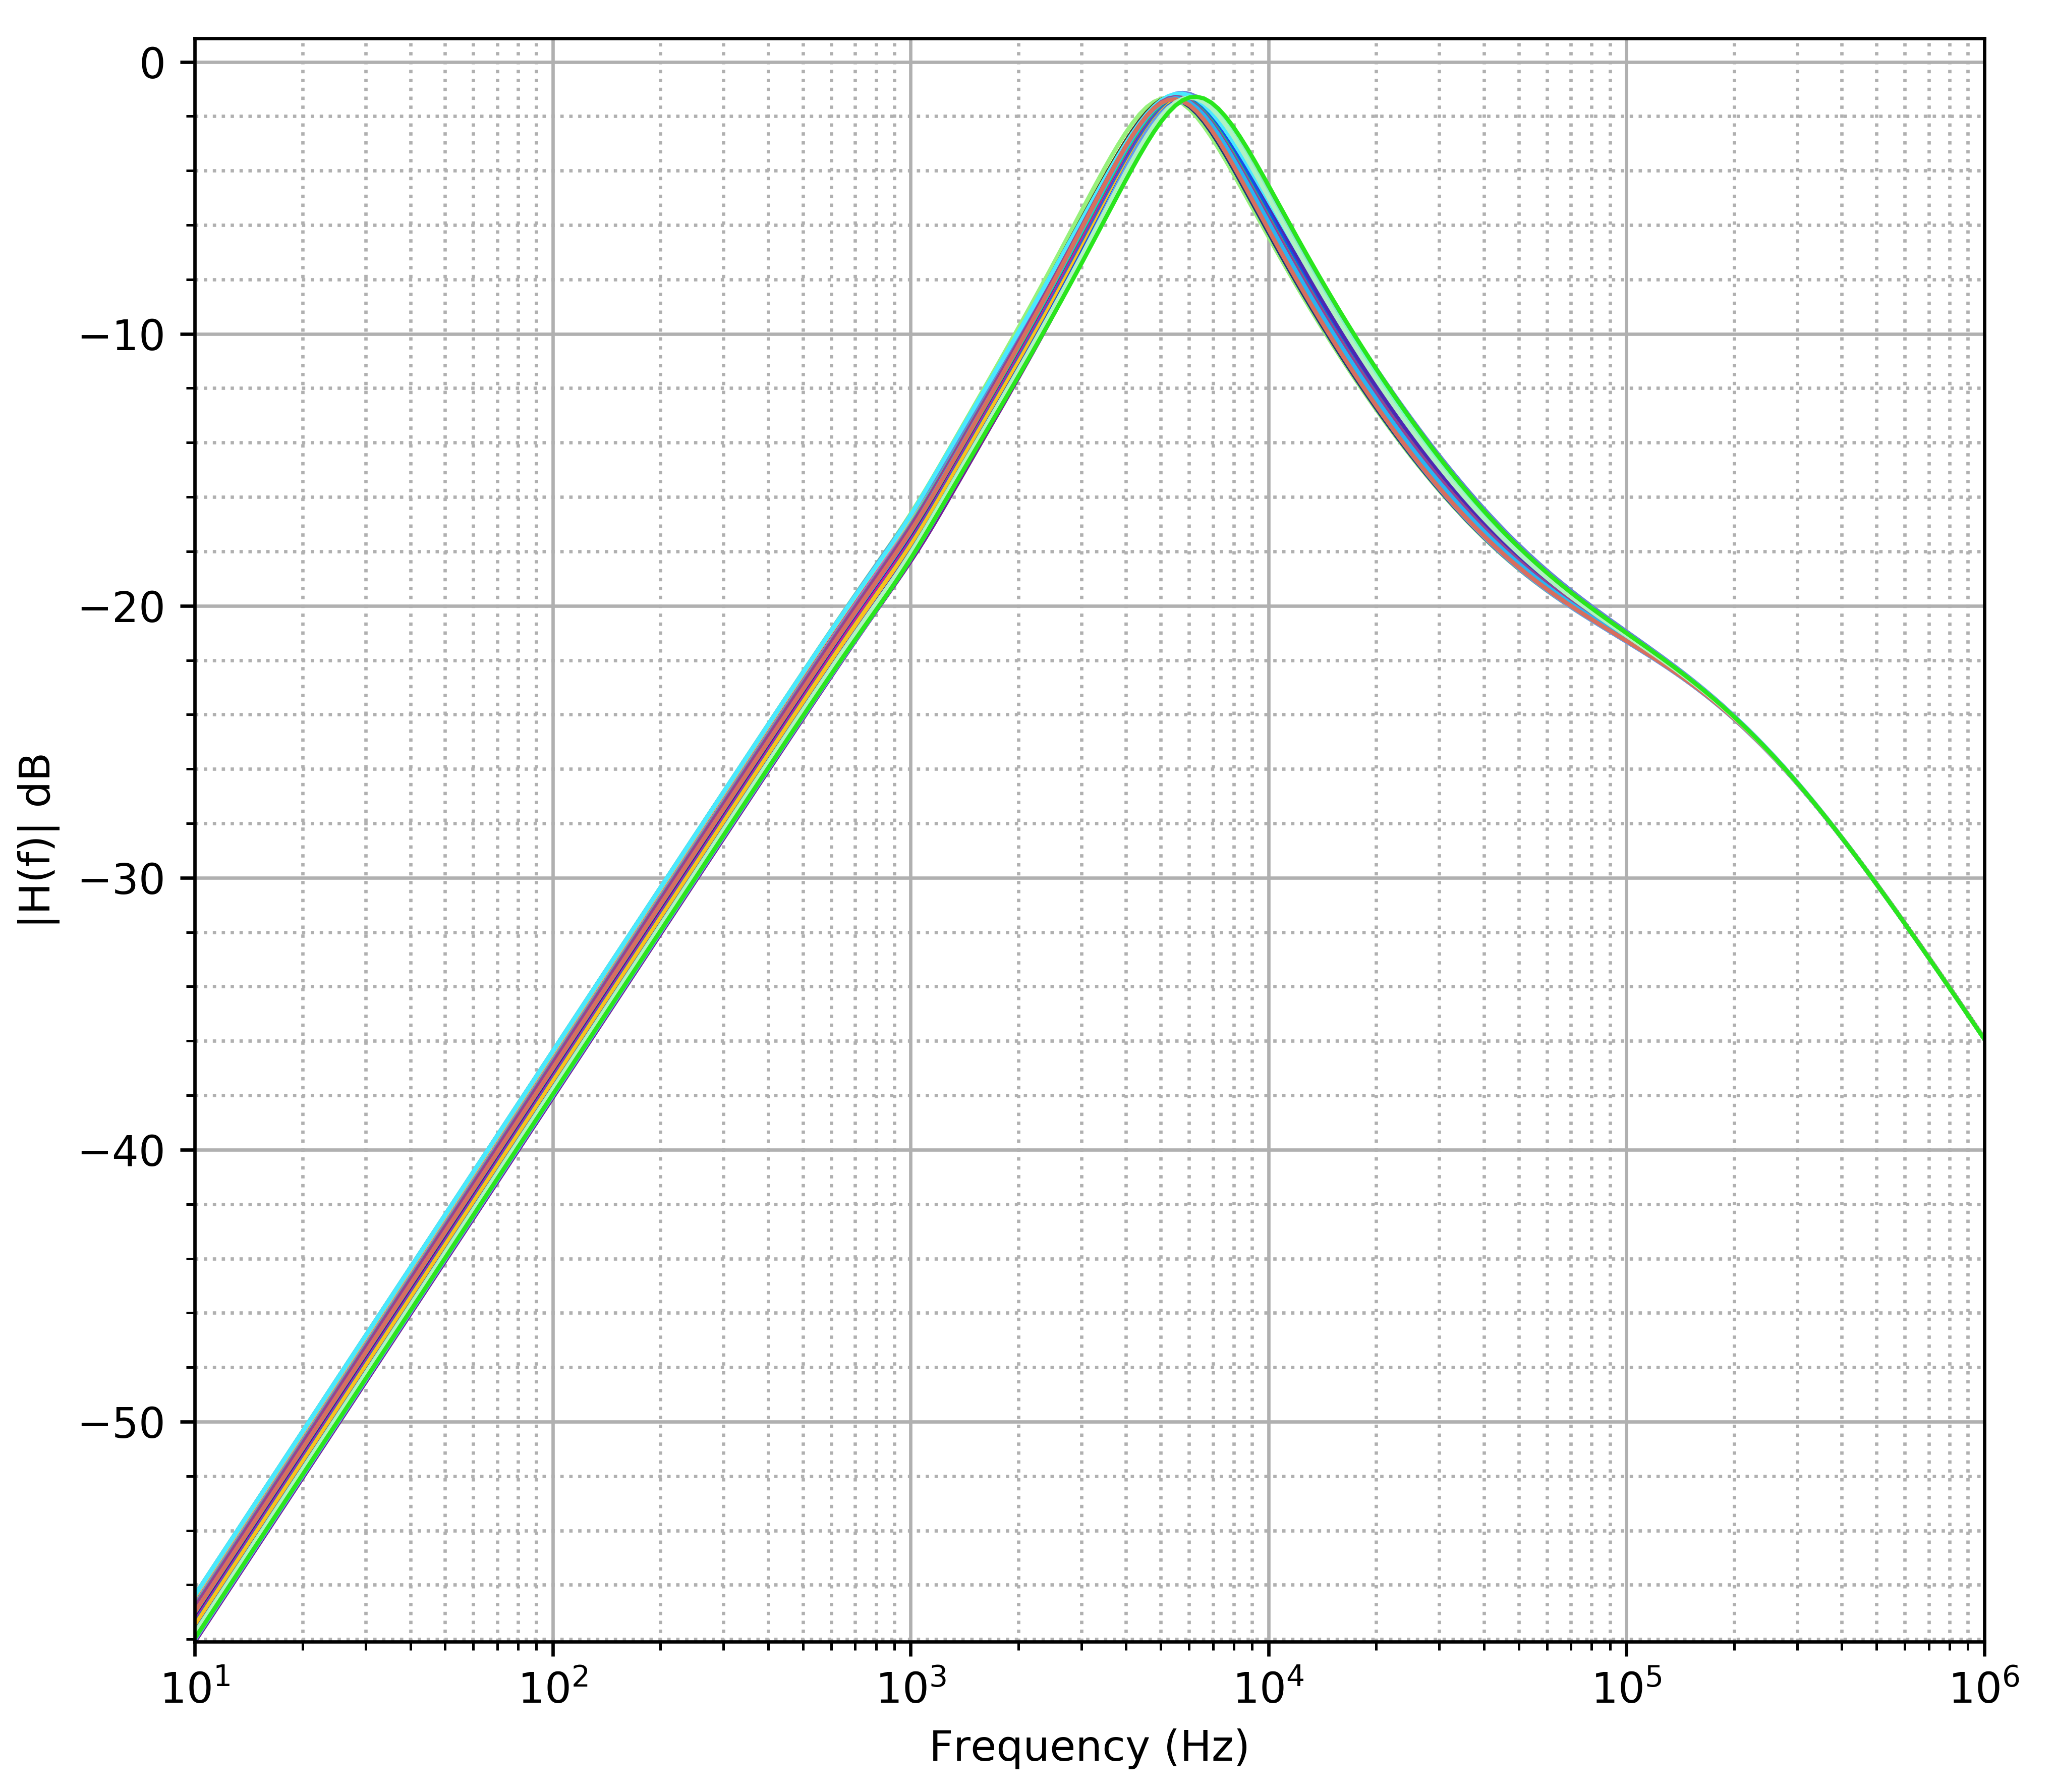
\includegraphics[scale=0.12]{../EJ2/Recursos/bd_montecarlo.png}    
    \caption{Respuesta en frecuencia en m\'odulo del filtro pasabanda}
    \label{fig:bd_montecarlo}
\end{figure}

\begin{figure}[H]
    \centering
        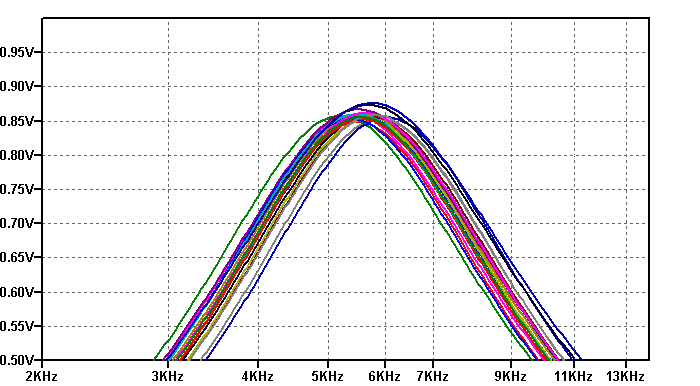
\includegraphics[scale=0.6]{../EJ2/Recursos/bp_montecarlo_frecuencia.png}
    \caption{Acercamiento en escala lineal de la respuesta en frecuencia}
    \label{fig:bp_montecarlo_frecuencia}
\end{figure}

\subsubsection{Resultados}
En las Fig. \ref{fig:bode_pasabanda_modulo} y \ref{fig:bode_pasabanda_fase} se puede observar los resultados del an\'alisis te\'orico, la simulaci\'on y las mediciones sobre la implementaci\'on
pr\'actica. Destacando que el punto de mayor ganancia sin superar los $0dB$ y la fase es $0^{\circ}$ se encuentra en la frecuencia $f = 5.7kHz$, habi\'endose desviado un $5\%$ respecto del valor ideal
por la tolerancia de los componentes.

\begin{figure}[H]
    \centering
        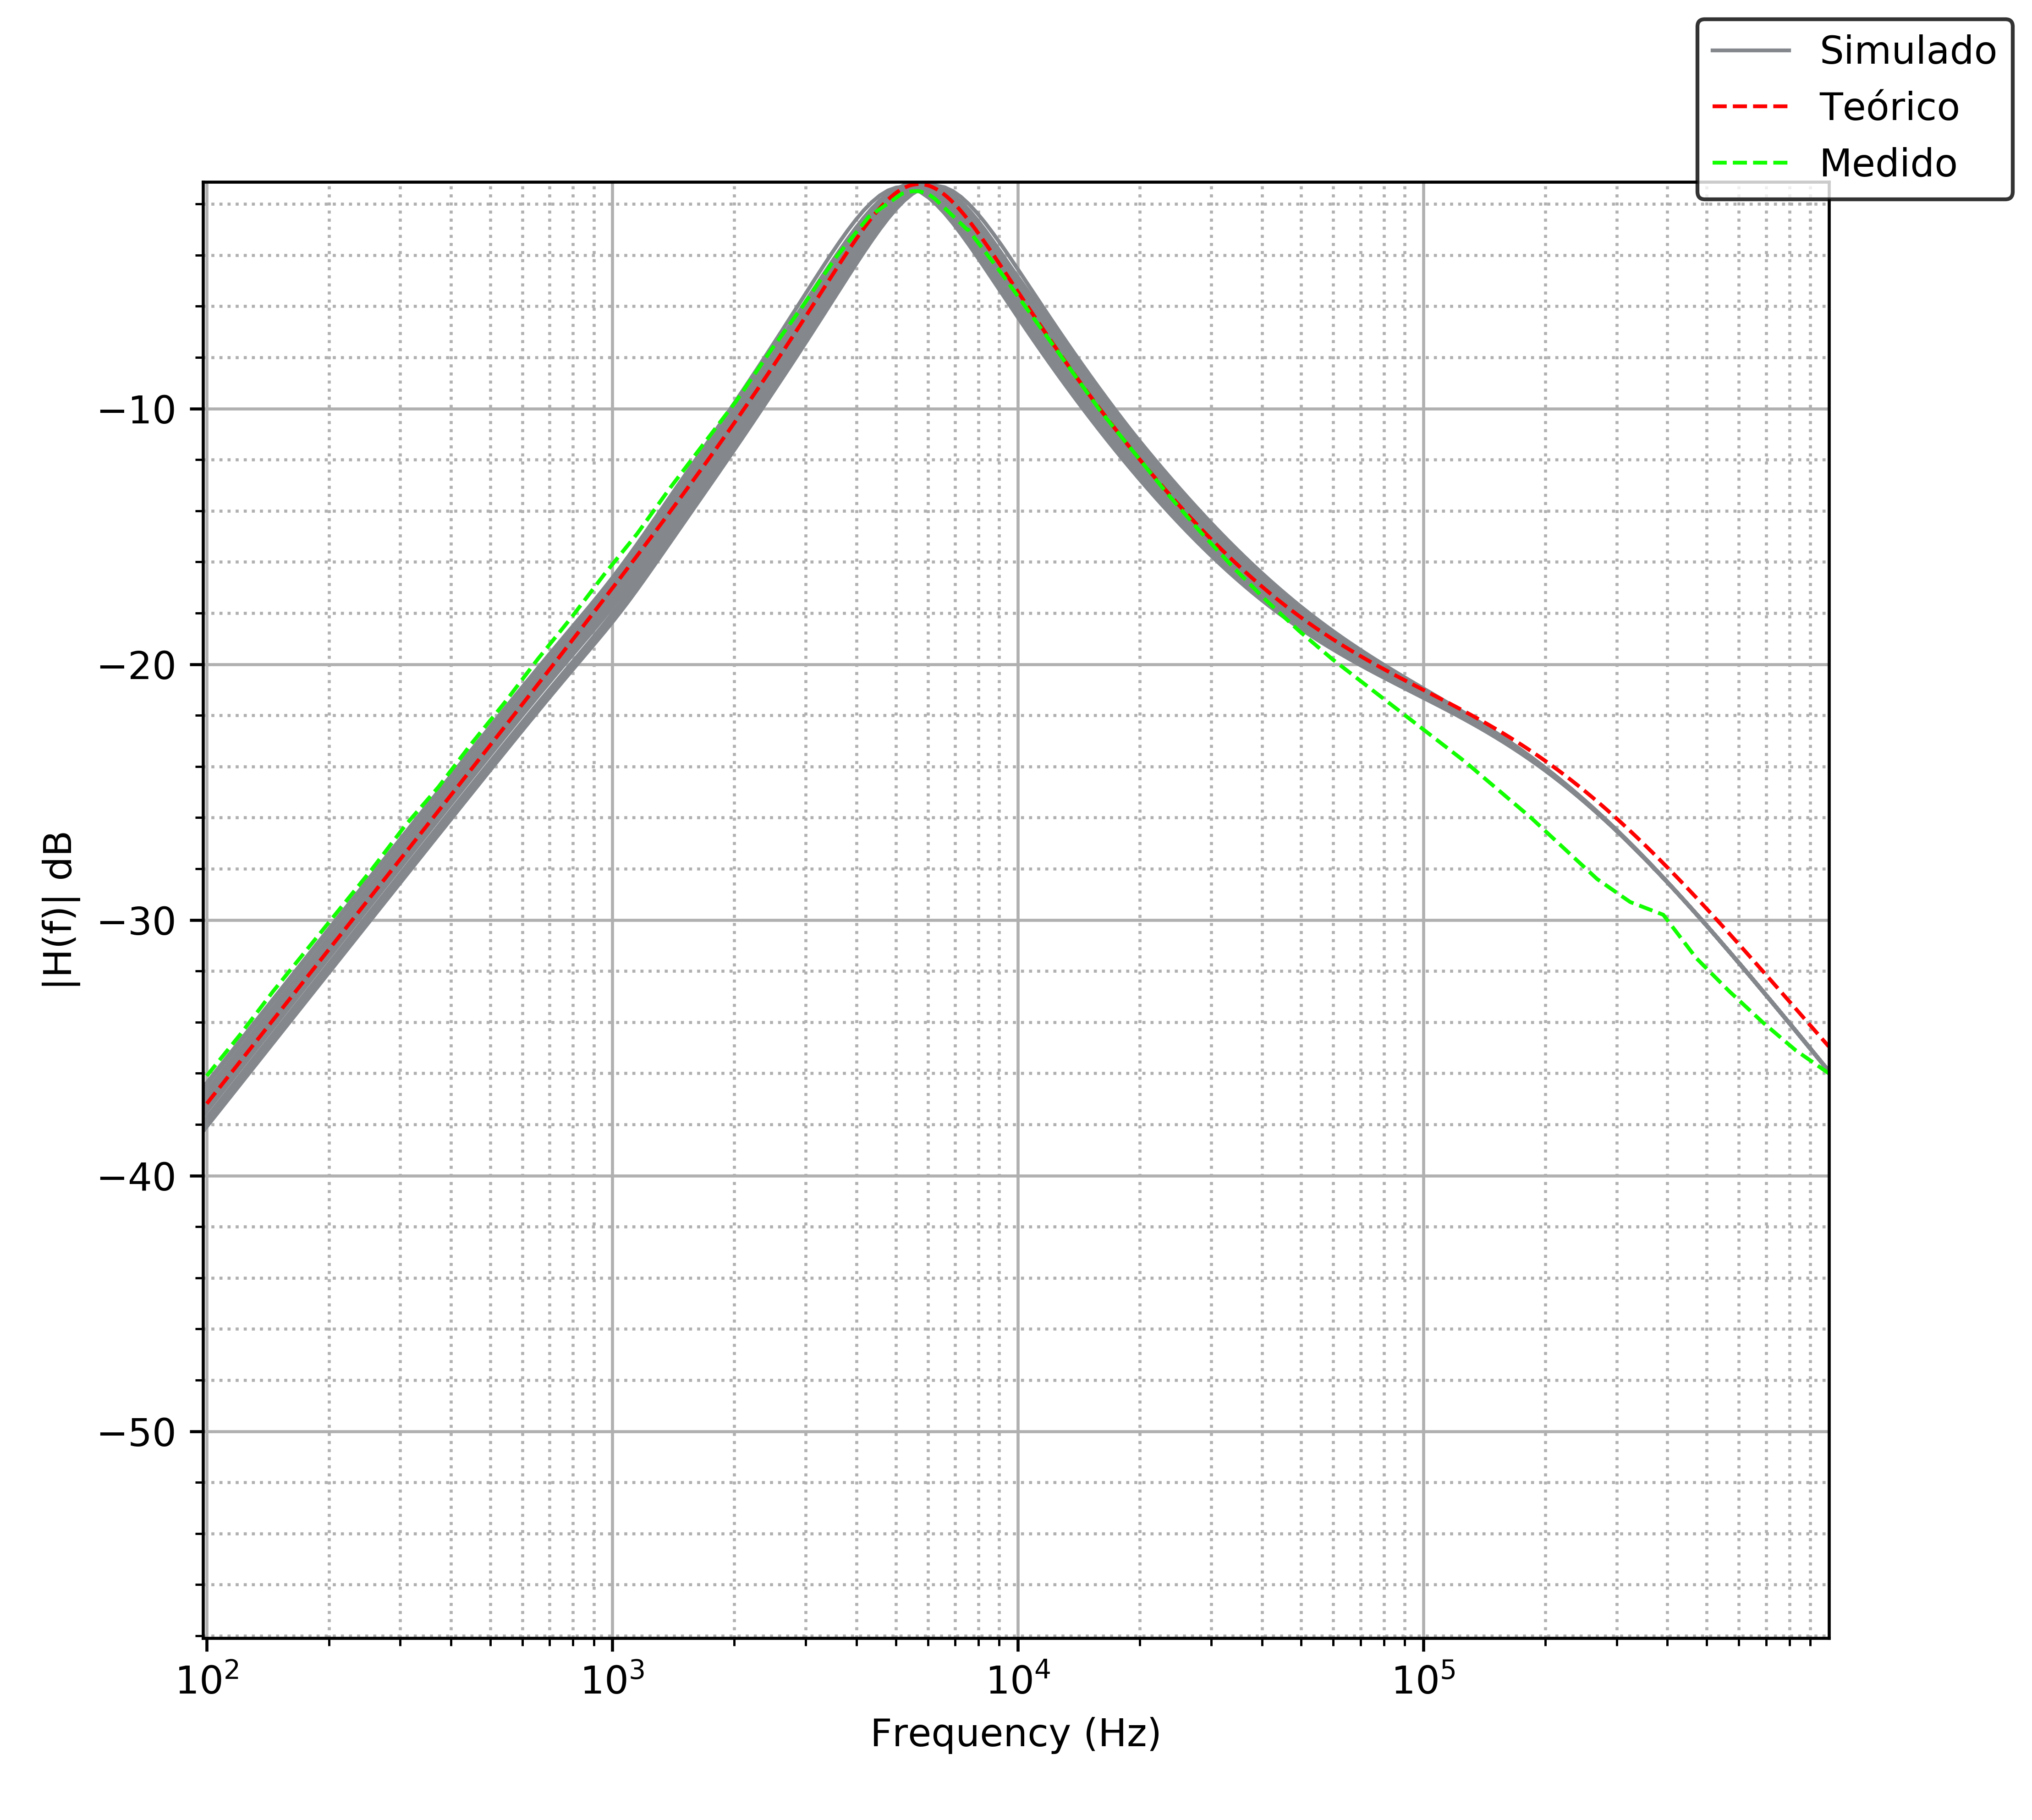
\includegraphics[scale=0.5]{../EJ2/Recursos/bode_pasabanda_modulo.png}
    \caption{Diagrama de bode en m\'odulo del filtro Pasabanda}
    \label{fig:bode_pasabanda_modulo}
\end{figure}

\begin{figure}[H]
    \centering
        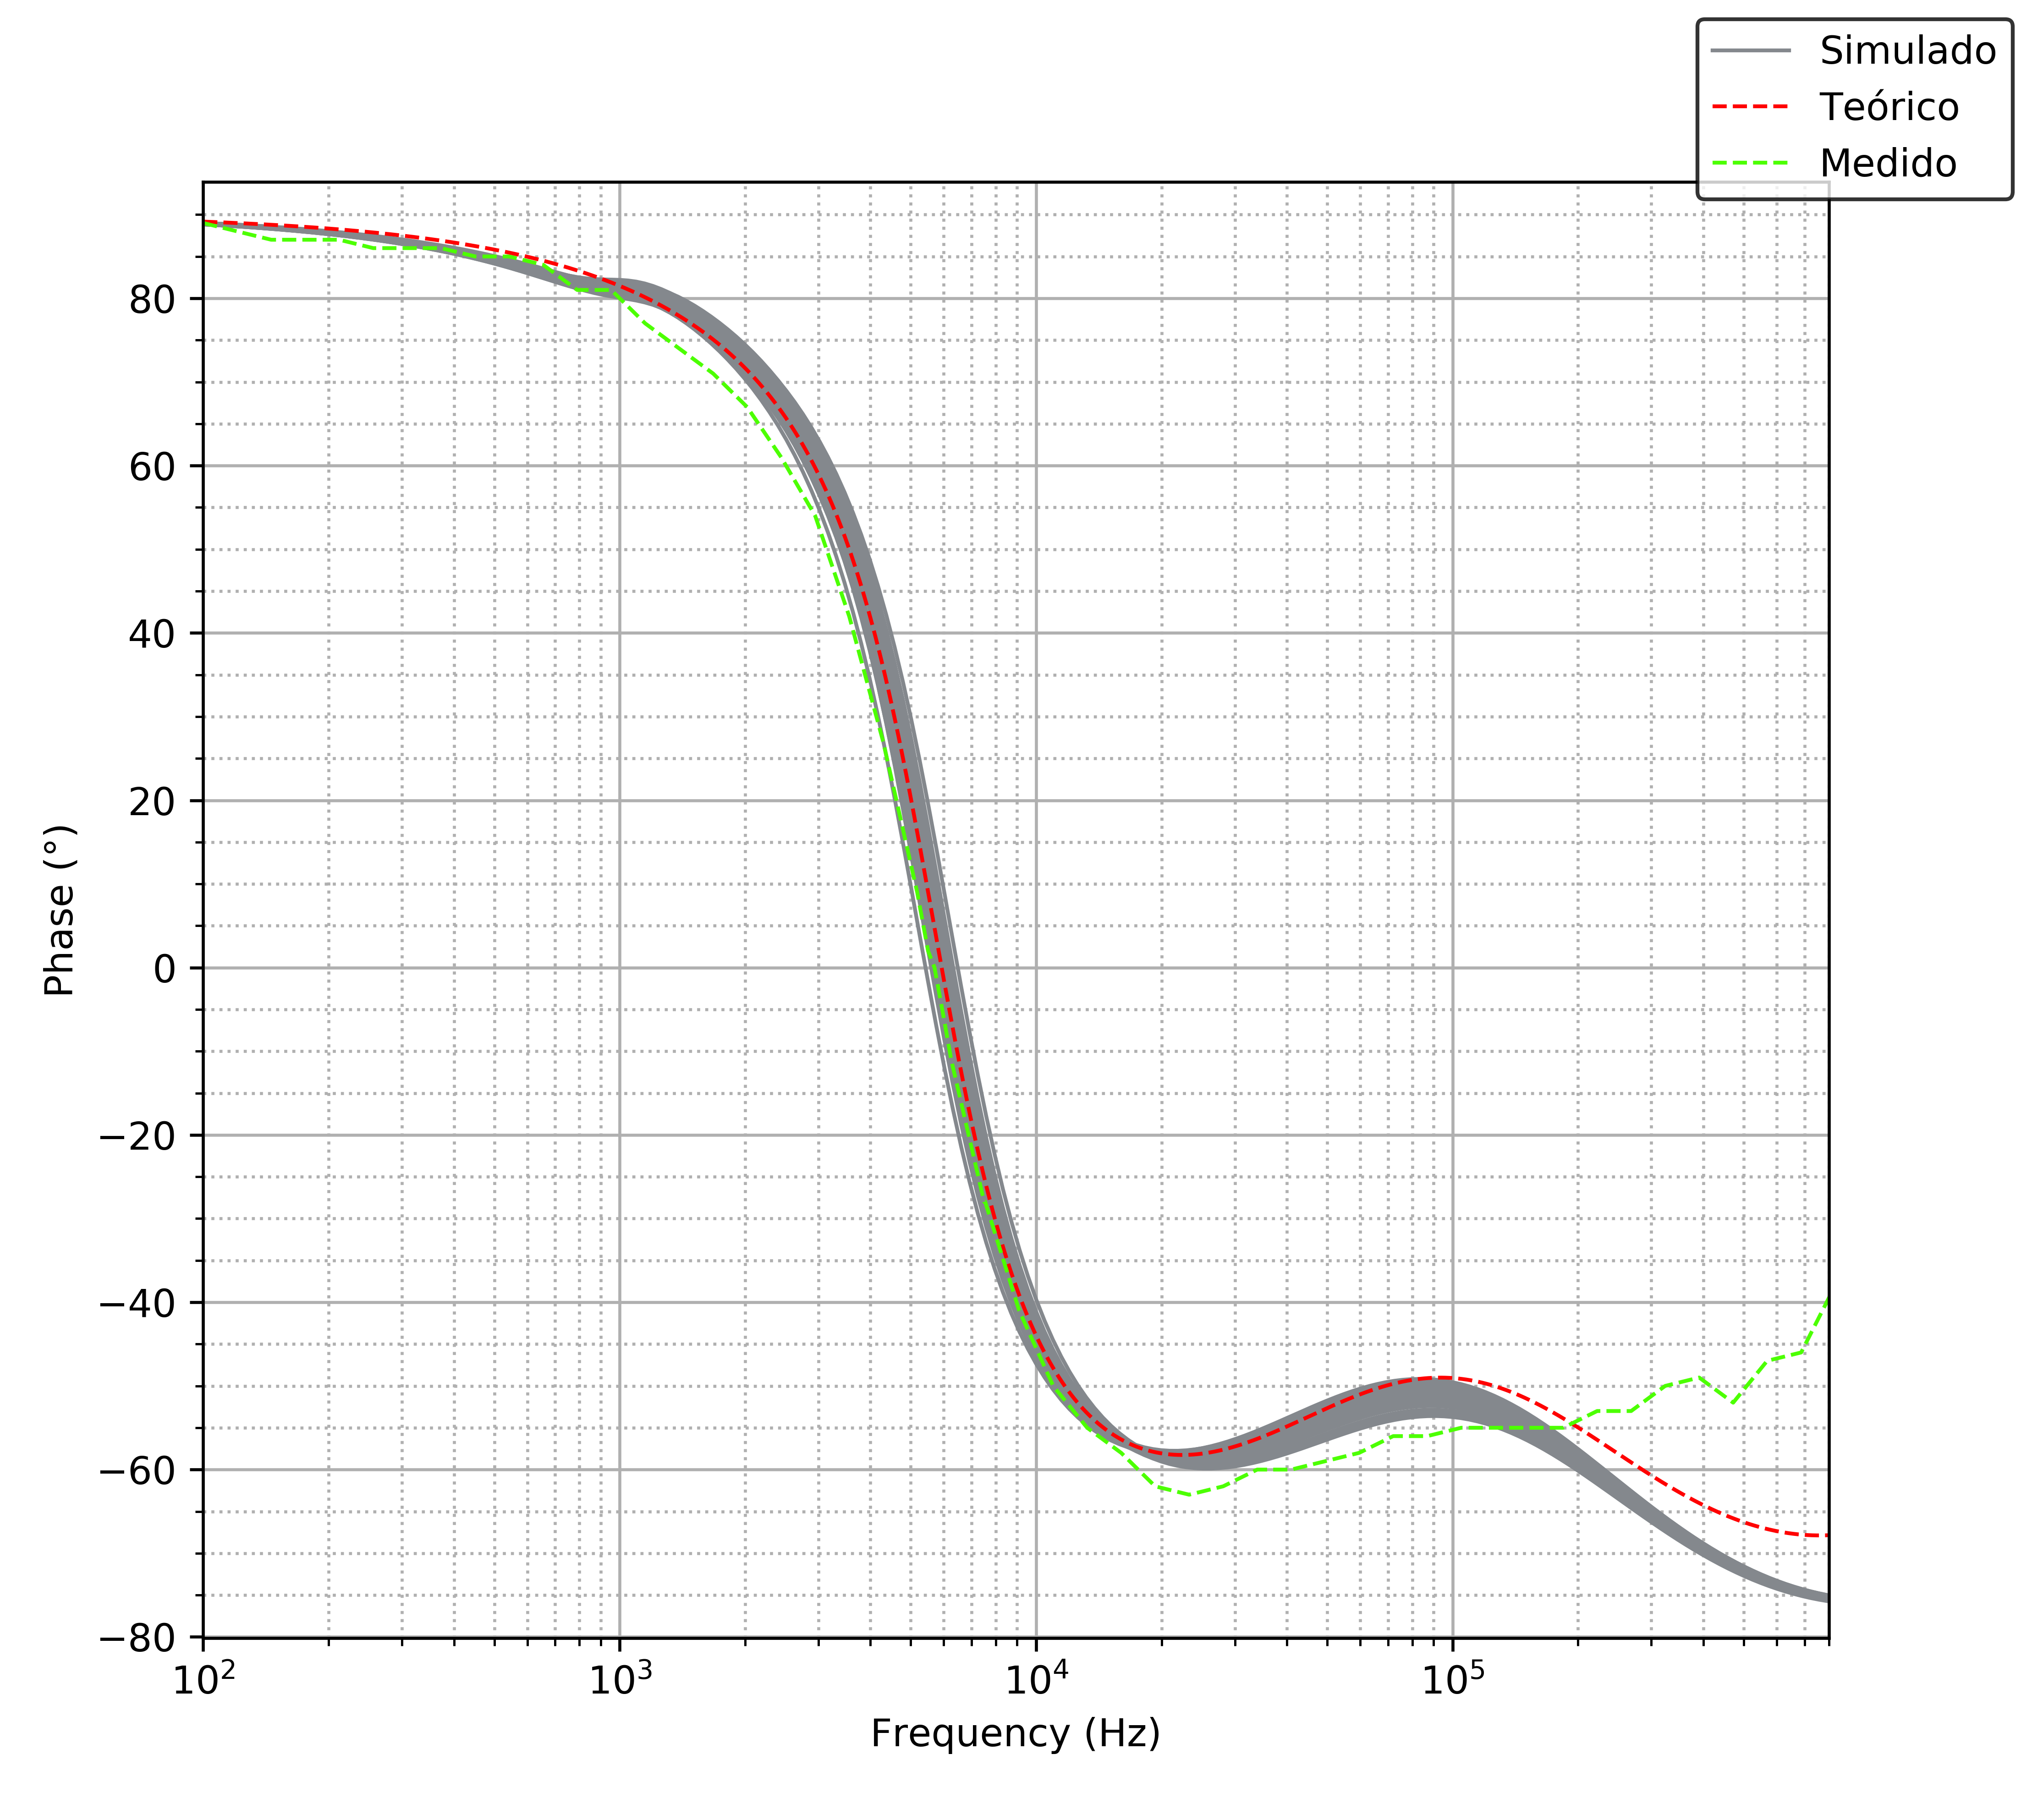
\includegraphics[scale=0.5]{../EJ2/Recursos/bode_pasabanda_fase.png}
    \caption{Diagrama de bode en fase del filtro Pasabanda}
    \label{fig:bode_pasabanda_fase}
\end{figure}

\subsection{Filtro Rechazabanda}
\subsubsection{Dise\~no de funci\'on transferencia}
Consid\'erese un sistema de segundo orden lineal, de tiempo invariante y bibo-estable, el cual debe caracterizar una respuesta en frecuencia propia de un filtro rechazabanda que aten\'ua todas las frecuencias entorno a una frecuencia determinada,
luego para poder modelizar matem\'aticamente dicho sistema a trav\'es de su funci\'on transferencia se emplea la siguiente ecuaci\'on. Cabe destacar que la expresi\'on ideal de un filtro rechazabanda careza de t\'ermino lineal en el numerador, no obstante
no ser\'a posible alcanzar tal condici\'on en la pr\'actica.

\begin{equation}
    H(s) = \frac{\left( \frac{s}{\omega_o} \right)^{2} + \frac{s}{Q_N \cdot \omega_o} + 1}{\left( \frac{s}{\omega_o} \right)^{2} + \frac{s}{Q_D \cdot \omega_o} + 1}    
\end{equation}

Para completar con este dise\~no del modelo matem\'atico empleado, se imponen como condiciones que la frecuencia de corte del filtro debe encontrarse tal que $\omega_o = 2\pi \cdot f_o =  2\pi \cdot 1kHz$. Adem\'as,
se busca que el numerador tenga un $\xi_N$ lo m\'as chico posible y cercano al valor nulo, mientras que el denominador se busca que tenga un valor lo m\'as cercano a la unidad posible.

\subsubsection{Dise\~no de circuito con Gyrator}
De igual forma que se fue realizando para los circuitos anteriores, se implementa la funci\'on transferencia del filtro rechazabanda replicando como se lo har\'ia con un circuito RLC, donde se busca reemplazar el comportamiento inductivo
por un Gyrator que lo simule, para ello primero se trabajan con equivalente y aproximaciones que permiten el dise\~no r\'apido y simplificado del circuito, posteriormente se analizan las caracter\'isticas no ideales del sistema obtenido y se buscan 
condiciones para maximizar el rango de operaci\'on de estas condiciones ideales.

\paragraph*{Circuito equivalente aproximado:} En la Fig. \ref{fig:equivalente_rechazabanda} se presenta el circuito equivalente de la implementaci\'on a realizar, para este caso se plantea la funci\'on transferencia y se obtiene luego
una funci\'on que se asemeja a la funci\'on deseada. 

\begin{figure}[H]
    \centering
    \includegraphics[scale=0.5]{../EJ2/Recursos/equivalente_rechazabanda.png}
    \caption{Circuito equivalente del rechazabanda}
    \label{fig:equivalente_rechazabanda}
\end{figure}

\begin{equation}
    H(s) = \frac{s^{2} \cdot LC + s \cdot C \cdot R_L + 1}{s^{2} \cdot LC + s \cdot C \cdot (R + R_L) + 1}    
\end{equation}

Entonces se obtiene que la frecuencia de corte del filtro se encuentra en $\omega_o = \frac{1}{\sqrt{LC}} = 2\pi \cdot 1kHz$, adem\'as se buscan los valores de los coeficientes de amortiguamiento tanto del numerador como denominador,
de esta forma se busca que imponiendo valores para los factores de calidad. Vale mencionar que los valores asignados a $Q_D$ y $Q_N$ son arbitrarios, no se posee un requisito espec\'ifico sobre c\'omo debe ser el ancho de banda del filtro.
Entonces, despejando de estas expresiones y buscando valores con el menor error posible, se llega a que $R_L = 100 \Omega$, $R = 1k \Omega$, $C = 100nF$ y $L = 0.2533H$.

\paragraph*{Circuito completo:} En la Fig. \ref{fig:circuito_rechazabanda} se ilustra el circuito completo de la aproximaci\'on considerada, empleando para ello un Gyrator. Al igual que se hizo hasta ahora,
se deben determinar valores para la capacidad $C_2$ y la resistencia $R_2$ para cumplir con el valor de inductancia requerido, adem\'as de con la condici\'on de dise\~no del Gyrator para maximizar el rango de operaci\'on, esto era,
$\omega << \frac{1}{C_2 \cdot R_L}$. Para esto se determina que $C_2 = 8.2nF$ y que $R_2 = 300k\Omega$.

\begin{figure}[H]
    \centering
    \includegraphics[scale=0.6]{../EJ2/Recursos/circuito_rechazabanda.png}
    \caption{Circuito completo del rechazabanda con el Gyrator}
    \label{fig:circuito_rechazabanda}
\end{figure}

\paragraph*{An\'alisis no ideal:} Para el an\'alisis no ideal se considera el amplificador operacional no ideal con un $A_{vol}$ finito con polo dominante, considerando que la impedancia de entrada muy alta con lo cual puede despreciarse la corriente
que circula hacia el interior del amplificador operacional. Se plantean ecuaciones para el circuito y se resuelven para llegar a la expresi\'on final sin aproximar de la funci\'on transferencia.

\begin{align*}
    & V_p = \frac{V_b \cdot R_2}{R_2 + \frac{1}{s \cdot C_2}} \\
    & A_{vol} = \frac{GBP}{s + \omega_p} \\
    & V_n = (V_p - V_n) \cdot A_{vol} \\
    & \frac{V_i - V_b}{R + \frac{1}{s \cdot C}} = \frac{V_b - V_n}{R_L} + \frac{V_b}{R_2 + \frac{1}{s \cdot C_2}} \\
    & V_o = V_b + \frac{(V_i - V_b) \cdot \frac{1}{s \cdot C}}{R + \frac{1}{s \cdot C}}
\end{align*}

\begin{align*}
    & a = \frac{C \cdot C_2 \cdot R_L \cdot R_2}{GBP + \omega_p}\\
    & b = C \cdot C_2 \cdot R_2 \cdot R_L + \frac{C \cdot R_L + C_2 \cdot (R_2 + R_L)}{GBP + \omega_p}\\
    & c = R_L \cdot (C + C_2) + \frac{1}{GBP + \omega_p} + \frac{C_2 \cdot R_2 \cdot \omega_p}{GBP + \omega_p}\\
    & \alpha = C \cdot C_2 \cdot \frac{R \cdot R_2 + R \cdot R_L + R_2 \cdot R_L}{GBP + \omega_p}\\
    & \beta = C \cdot C_2 \cdot R_L \cdot ( R + R_2) + \frac{C \cdot C_2 \cdot R \cdot R_2 \cdot \omega_p}{GBP + \omega_p} + \frac{C \cdot (R + R_L) + C_2 \cdot(R_2 + R_L) }{GBP + \omega_p}\\
    & \gamma = C \cdot(R + R_L) + C_2 \cdot R_L + \frac{1 + C_2 \cdot R_2}{GBP + \omega_p} \\
    & H(s) = \frac{a \cdot s^{3} + b \cdot s^{2} + c \cdot s + 1}{\alpha \cdot s^{3} + \beta \cdot s^{2} + \gamma \cdot s + 1} \\
\end{align*}

Luego considerando que $GBP << \omega_p$, $\frac{GBP}{GBP + \omega_p} \approx 1$, $\frac{\omega_p}{GBP + \omega_p} \approx \frac{\omega_p}{GBP}$, 
$\omega << GBP$, $\omega << \frac{1}{C \cdot R_L}$, $\omega << \frac{1}{C_2 \cdot R_2}$ y que $R_2 >> R > R_L$ luego se llega a una aproximaci\'on de la versi\'on ideal de la funci\'on.

\begin{equation}
    H(s) \approx \frac{C \cdot C_2 \cdot R_2 \cdot R_L \cdot s^{2} + s \cdot C \cdot R_L + 1}{C \cdot C_2 \cdot R_2 \cdot R_L \cdot s^{2} + s \cdot C \cdot (R + R_L) + 1}    
\end{equation}

\subsubsection{Verificaci\'on del dise\~no}
Se realiza la simulaci\'on del circuito en LTSpice con un an\'alisis de Monte Carlo para considerar la dispersi\'on del valor de los componentes en la realidad.
Los resultados se pueden observar en las figuras \ref{fig:br_montecarlo} y \ref{fig:br_montecarlo_frecuencia}.

\begin{figure}[H]
    \centering
        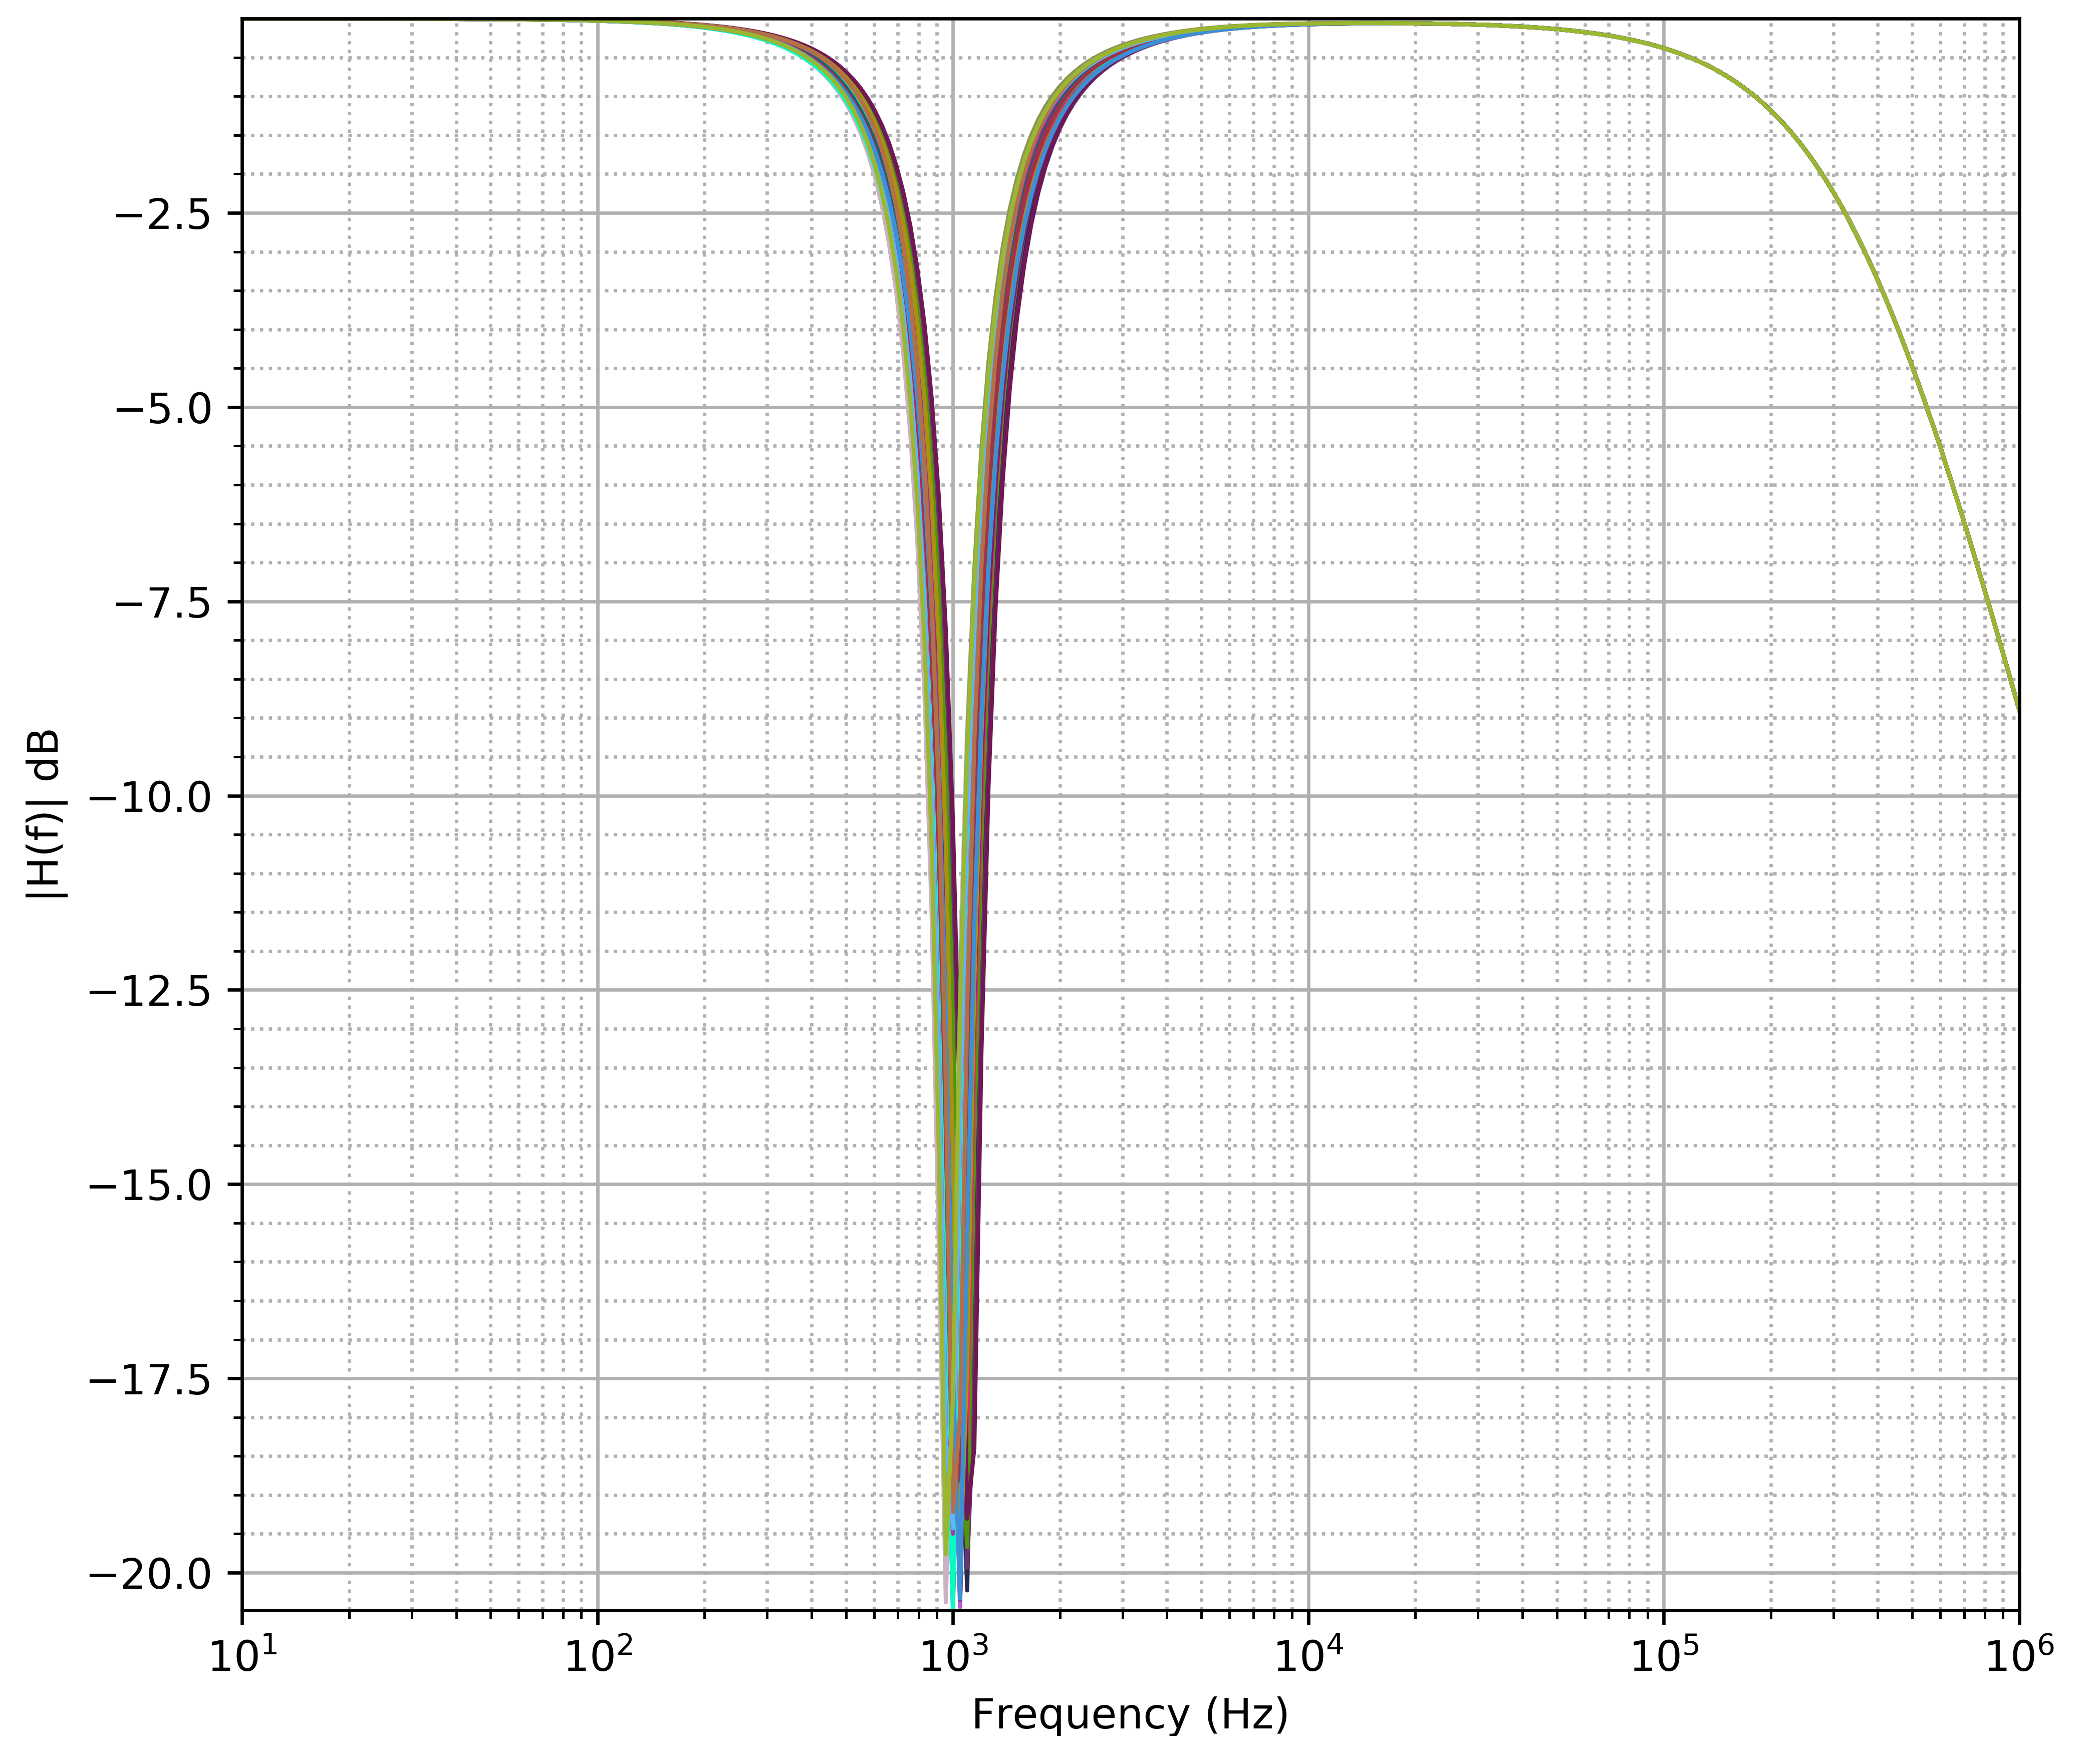
\includegraphics[scale=0.12]{../EJ2/Recursos/br_montecarlo.png}
    \caption{Respuesta en frecuencia en m\'odulo del filtro rechazabanda}
    \label{fig:br_montecarlo}
\end{figure}

\begin{figure}[H]
    \centering
    \begin{tabular}{c c}
        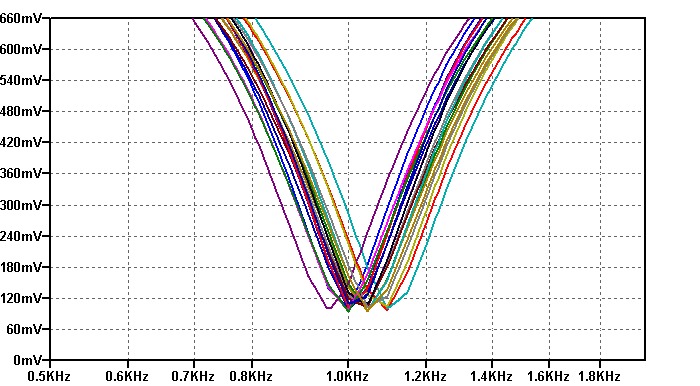
\includegraphics[scale=0.6]{../EJ2/Recursos/br_montecarlo_frecuencia.png}
    \end{tabular}
    \caption{Acercamiento a la frecuencia del filtro rechazabanda}
    \label{fig:br_montecarlo_frecuencia}
\end{figure}

\subsubsection{Resultados}
En las Fig. \ref{fig:bode_rechazanda_modulo} y \ref{fig:bode_rechazabanda_fase} se puede observar los resultados de constrastar el an\'alisis te\'orico,
la simulaci\'on y la implementaci\'on pr\'actica. Adem\'as, se midi\'o que el punto de menor ganancia de la respuest se da en la frecuencia $f = 920Hz$ con una ca\'ida
de $-15.5dB$ y una fase de $0^{\circ}$.

Nuevamente puede observarse que para frecuencias altas el Gyrator deja de emular una bobina por la baja componente reactiva que produce el capacitor
como ya se explic\'o inicialmente en el an\'alisis, de ah\'i que para tales frecuencias se produce una desviaci\'on respecto de lo esperado idealmente.

\begin{figure}[H]
    \centering
        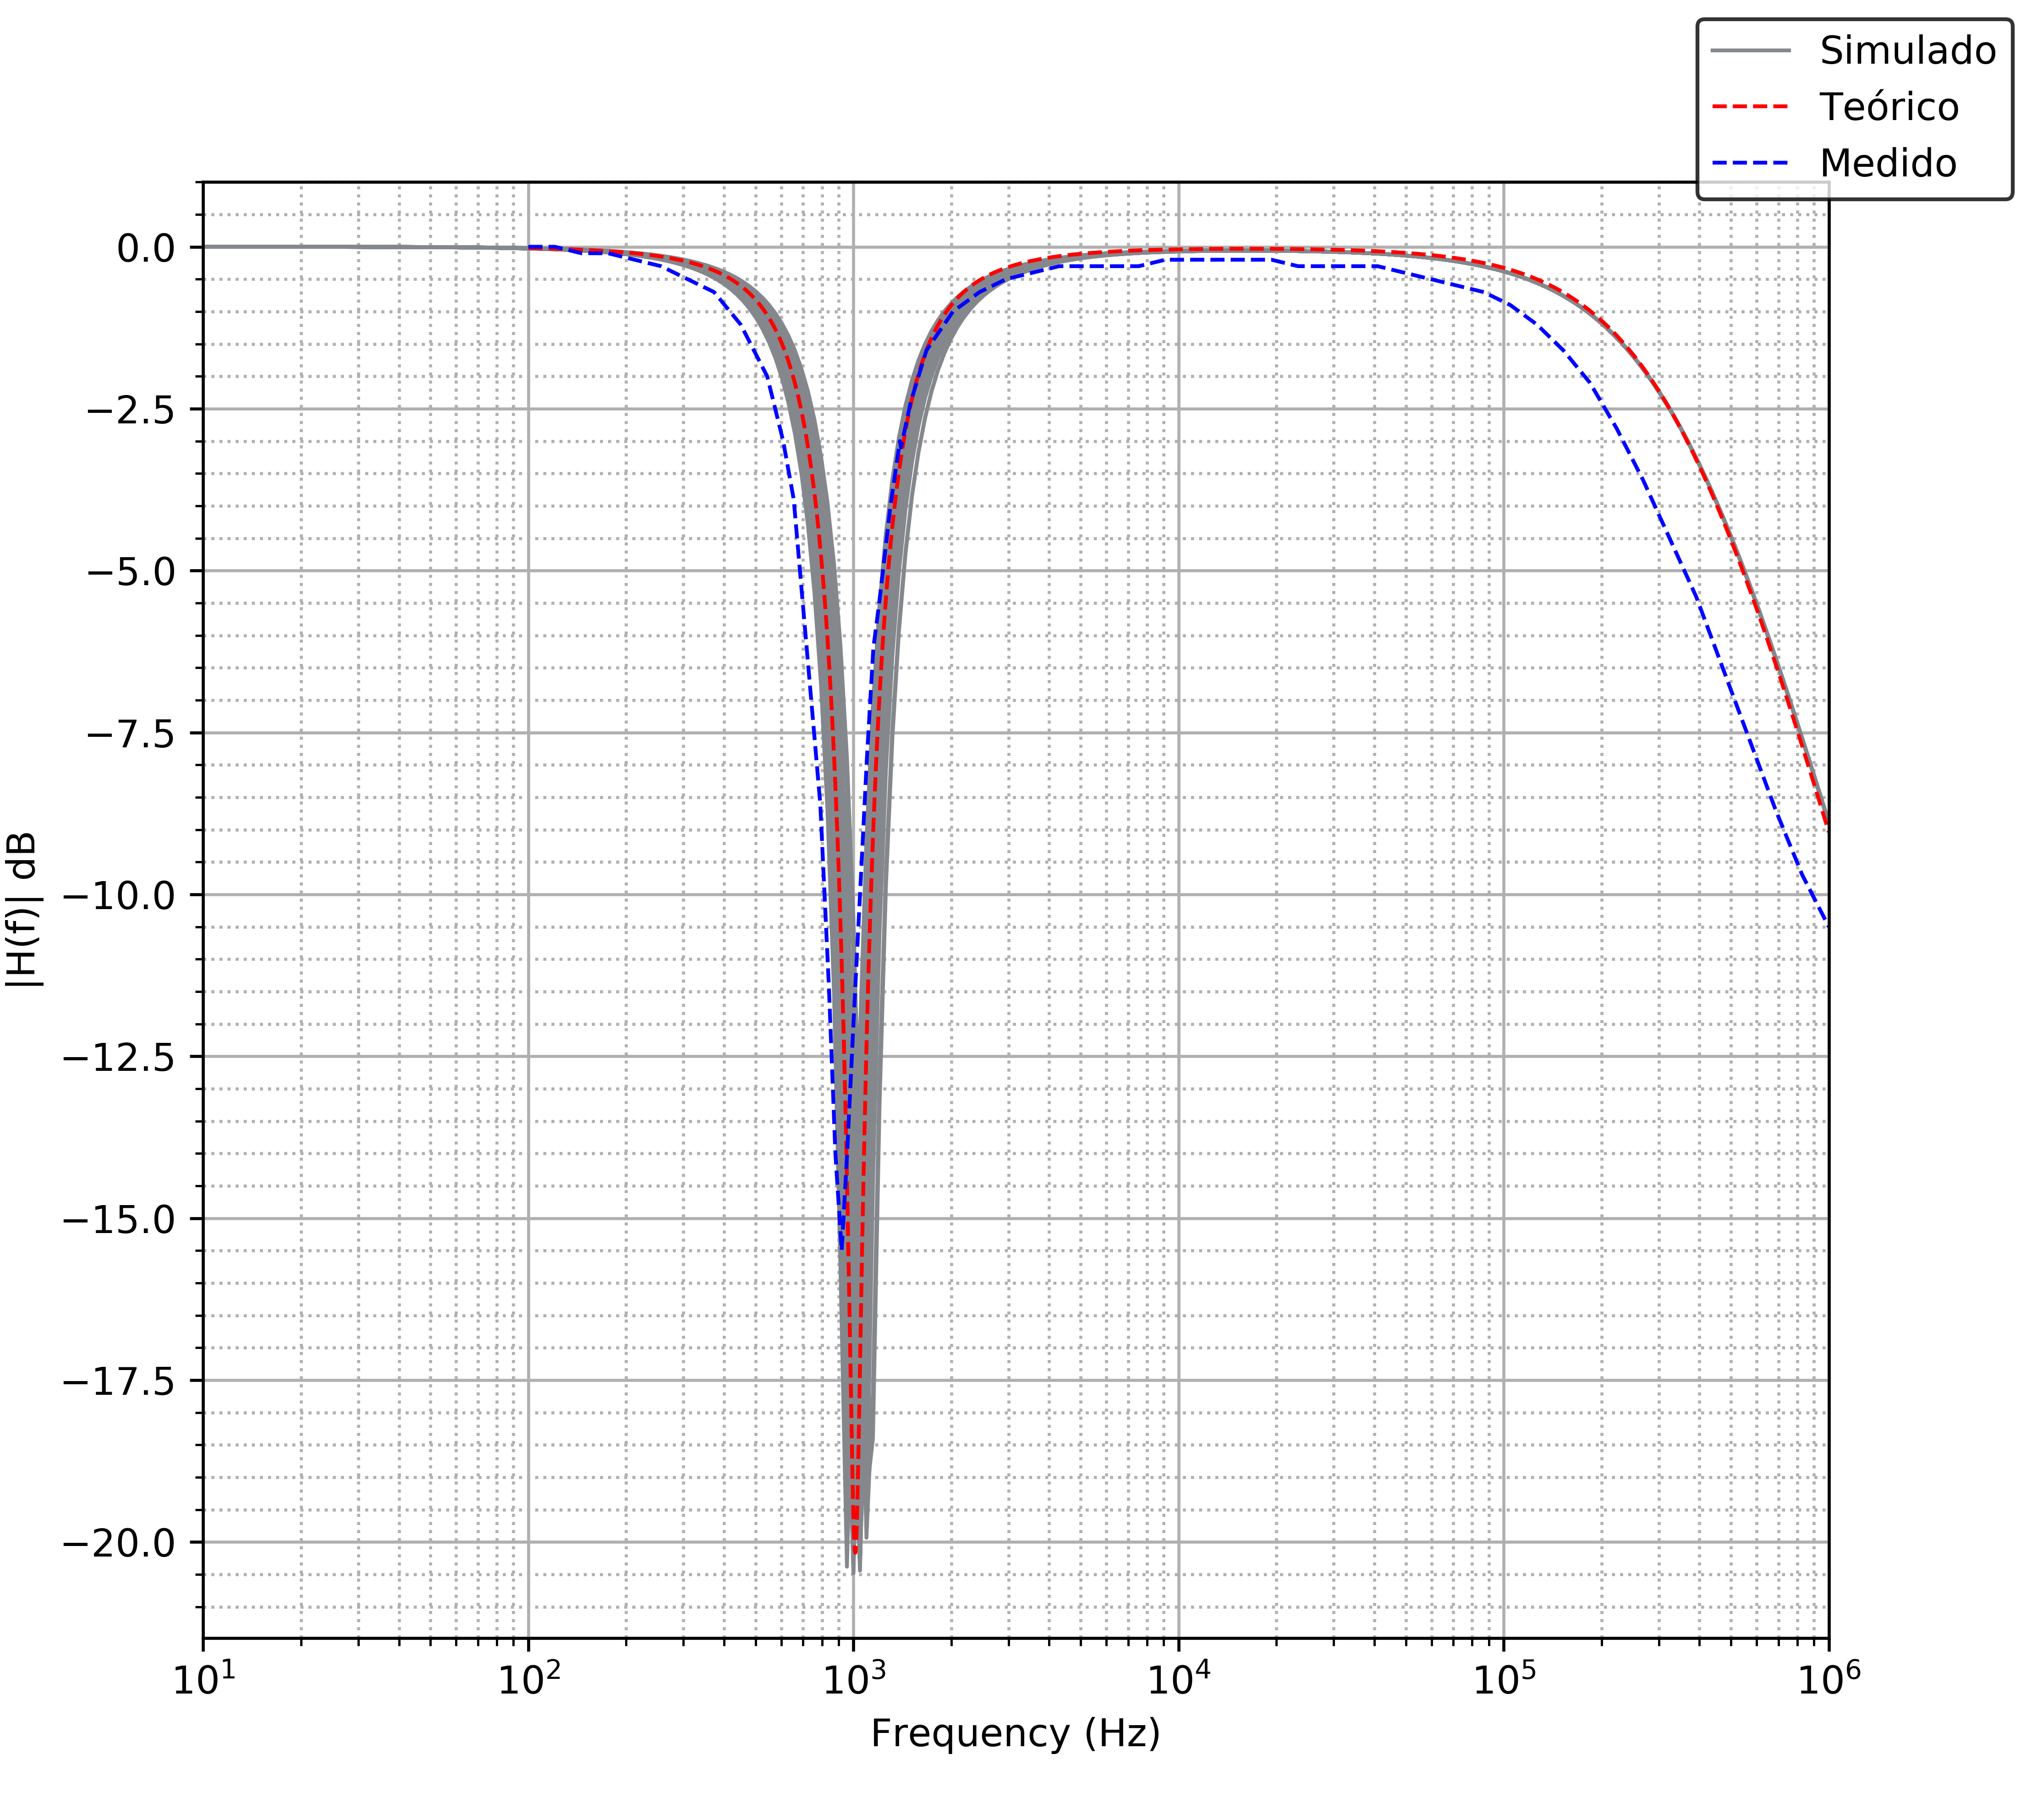
\includegraphics[scale=0.5]{../EJ2/Recursos/bode_rechazabanda_modulo.png}
    \caption{Diagrama de bode en m\'odulo del filtro rechazabanda}
    \label{fig:bode_rechazanda_modulo}
\end{figure}

\begin{figure}[H]
    \centering
        \includegraphics[scale=0.5]{../EJ2/Recursos/bode_rechazabanda_fase.png}
    \caption{Diagrama de bode en fase del filtro rechazabanda}
    \label{fig:bode_rechazabanda_fase}
\end{figure}

\subsection{Implementaci\'on pr\'actica}

\subsubsection{Selecci\'on del amplificador operacional}
Para la implementaci\'on pr\'actica de los circuitos, habiendo ya definido los valores de los componentes, es necesario seleccionar un modelo de amplificador operacional a partir de 
consideraciones o suposiciones realizadas en el an\'alisis te\'orico. Por lo tanto, lo primero a realizar es definir los requisitos que son impuestos sobre dicho modelo.

\paragraph*{Impedancia de entrada:} Para todo an\'alisis te\'orico se consider\'o la impedancia de entrada del amplificador lo suficientemente grande para poder despreciar las corrientes que hacia este se desviaban.
Para poder determinar cu\'anto tan grande debe ser, es necesario compararla con la impedancia colocada en la resistencia $R_2$ de los circuitos del Gyrator utilizados, y el valor m\'as grande entre ellos es de $R_2 = 820 k \Omega$, con lo cual
es necesario una impedancia de entrada al amplificador operancional que sea mucho mas grande que esta, para poder despreciar las corrientes de p\'erdida que se produzcan.

\paragraph*{Producto de ganancia y ancho de banda GBP:} Este valor que fue tomado en frecuencia angular, se requiere que sea mucho mayor que las frecuencias de operaci\'on, pero al mismo tiempo se pidi\'o que sea superior a las frecuencias de corte de los filtros
para llevar las expresiones no ideales a sus formas aproximadas, por lo tanto entre todos los filtros el requisito m\'as demandante para este par\'ametro implica que $GBP >> 2 \pi \cdot 2.97MHz$. Este n\'umero resulta de comparar cada conjunto de aproximaciones realizadas
en el an\'alisis no ideal de cada filtro, tomando el peor caso, el cual fue resultante de pedir que en el filtro pasabajos GBP fuera lo suficientemente grande para que no afectara a la frecuencia de $10,5kHz$.

\paragraph*{Slew rate, corrientes de bias y tensión de polarización:} En el an\'alisis de los filtros no fueron tenidos en cuenta estos aspectos, por lo tanto no hay un requisito inmediato sobre estos valores, aunque s\'i resulta necesario
reducir al m\'aximo el efecto del as corrientes de bias para limitar la componente de continua, as\'i como evitar posibles distorsiones de salida ya sea por saturaci\'on y pendiente m\'axima, es decir, slew rate. Por lo tanto en caso de tener diversas opciones
que cumplan con los requisitos previos, se optar\'a por la de mejor cualidades en estos aspectos.

\paragraph*{Encapulado:} Es necesario emplear \'unicamente un circuito integrado que disponga de los cuatro amplificadores operacionales necesarios.

\begin{table}[H]
    \centering
    \begin{tabular}{c c c c}
        $Modelo$ & $Z_{in}(s)$ & $GBP$ & $Slew Rate$ \\
        \hline \\
        $LF346$ & $10^{12} \Omega$ & $2 \pi \cdot 3MHz$ & $13 \frac{V}{\mu S}$ \\
        $TL084$ & $10^{12} \Omega$ & $2 \pi \cdot 3MHz$ & $13 \frac{V}{\mu S}$ \\
        $TL074$ & $10^{12} \Omega$ & $2 \pi \cdot 3MHz$ & $13 \frac{V}{\mu S}$ \\
        $LM324$ & $No informa$ & $2 \pi \cdot 1MHz$ & $0.5 \frac{V}{\mu S}$ \\
        \hline 
    \end{tabular}
\end{table}

En la tabla se pueden observar las variantes disponibles y finalmente se escoge el TL084.

\subsubsection{Esquem\'atico del circuito}

\begin{figure}[H]
    \centering
    \includegraphics[scale=1]{../EJ2/Recursos/esquematico_complementario.PNG}
    \caption{Esquem\'atico conexiones y puntos de medici\'on}
    \label{fig:esquematico_complementario}
\end{figure}

\begin{figure}[H]
    \centering
    \begin{tabular}{c c}
        \includegraphics[scale=1]{../EJ2/Recursos/esquematico_low_pass.PNG} &
        \includegraphics[scale=1]{../EJ2/Recursos/esquematico_high_pass.PNG} \\
        \includegraphics[scale=1]{../EJ2/Recursos/esquematico_band_pass.PNG} &
        \includegraphics[scale=1]{../EJ2/Recursos/esquematico_notch.PNG} 
    \end{tabular}
    \caption{Esquem\'atico de circuitos filtros}
    \label{fig:esquematico_filtros}
\end{figure}

\subsubsection{Dise\~no del PCB y vista 3D}

\begin{figure}[H]
    \centering
        \begin{tabular}{c c}
            \includegraphics[scale=0.5]{../EJ2/Recursos/top_3d.PNG} &
            \includegraphics[scale=0.5]{../EJ2/Recursos/bottom_3d.PNG}
        \end{tabular}
    \caption{Vista 3D del dise\~no del PCB en Altium Designer}
    \label{fig:vista_3d}
\end{figure}

	\newpage
	\section{Amplificador de instrumentaci\'on} 
\subsection{Introducci\'on}
\paragraph{Amplificador diferencial}
Un amplificador diferencial es un dispositivo que amplifica la $\textit{diferencia}$ de las se\~nales en sus entradas. El principio de funcionamiento de este amplificador es la de, asumiendo que el ruido introducido en sus entradas es igual para todas ellas,  la diferencia entre las se\~nales comunes, en modo com\'un(el ruido por ejemplo), es nula, por lo tanto es atenuada infinitamente. Se obtiene a la salida la amplificaci\'on de las se\~nales en modo diferencial.
Se muestra en la Figura \ref{fig:AMP_DIF}  el amplificador diferencial con un modelo de las entradas en modo com\'un y modo diferencial.
\begin{figure}[H]

    \centering
    \includegraphics[width=0.5\textwidth]{../EJ3/Recursos/AMP_DIF}
    \caption{Amplificador diferencial b\'asico}
    \label{fig:AMP_DIF}
\end{figure}

En la realidad no se consigue el funcionamiento ideal descripto anteriormente, luego es necesario introducir los conceptos de $A_{DM}$, $A_{CM}$ y $CMRR$. $A_{DM}$ indica la ganancia en modo diferencial del circuito, $A_{CM}$ indica la ganancia en modo com\'un y $CMRR$ o Common Mode Rejection Ratio indica la relaci\'on entre ambas, lo que muestra cuantitativamente cuanto rechaza el circuito, se\~nales en modo com\'un. Este se calculado como se muestra en \ref{eq:CMRR}

 \begin{equation}
    CMRR=20 \cdot \log \left| \frac{A_{DM}}{A_{CM}} \right|
    \label{eq:CMRR}
 \end{equation}
\paragraph{Amplificador de instrumentaci\'on}
El amplificador de instrumentaci\'on es un amplificador diferencial de precisi\'on que parte de los conceptos explicados anteriormente. Sin embargo se introduce a su entrada una etapa sim\'etrica previa, con entrada y salida diferencial, que aumenta la impedancia de entrada y permite dividir la ganancia en dos etapas. Las caracter\'isticas pricipales de este circuito son su alta impedancia de entrada, una baja impedancia de salida y un alto $CMRR$.

\subsection{An\'alisis te\'orico}
Se presenta en la Figura \ref{fig:AMP_INST} el amplificador de instrumentaci\'on analizado en esta secci\'on.
\begin{figure}[H]

    \centering
    \includegraphics[width=0.5\textwidth]{../EJ3/Recursos/AMP_INST}
    \caption{Amplificador de instrumentaci\'on utilizado}
    \label{fig:AMP_INST}
\end{figure}
Si se compara el circuito de la figura, con la configuraci\'on de amplificador de instrumentaci\'on descripta anteriormente, se observa que se agrega el amplificador operacional $U4$. La funci\'on de este \'ultimo es la de fijar un potencial cercano a los $0V$ en el nodo $VA$, conservando la simetria. Esto es de suma importancia porque, con esta condici\'on y aplicando el Teorema de Bartlett con el modelo de modo com\'un, es posible analizar el circuito como se muestra en la Figura \ref{fig:SIMETRICO} 
\begin{figure}[H]

    \centering
    \includegraphics[width=0.5\textwidth]{../EJ3/Recursos/SIMETRICO}
    \caption{Circuito equivalente con realimentaci\'on, para modo com\'un}
    \label{fig:SIMETRICO}
\end{figure}
Se puede ver entonces que, trabajando en modo com\'un, la etapa de la entrada amplifica igual en ambas entradas y luego es atenuado por la etapa restadora.
\subsubsection{Asumiendo amplificadores operacionales ideales}
Se presenta en \ref{eq:sist_ideal} el sistema de ecuaciones del que se parte para obtener la respuesta del sistema.
\begin{equation}
        \left\{
            \begin{array}{llll}
                
                V_{o2} = 0 &\\
                
                V_{o1} = V_{1}\cdot \left(1+\frac{R_3}{R_4}\right) - V_A\cdot\frac{R_3}{R_4}\\
                
                V_A = V_2\cdot \left(1+\frac{R_6}{R_7}\right)\\
                
                V_{out} = \left(1+\frac{R_2}{R_1}\right)\cdot V_{o2} -  \frac{R_2}{R_1} \cdot V_{o1}
            \end{array}
        \right.
  \label{eq:sist_ideal}
\end{equation}
Se obtiene de ese sistema entonces la tensi\'on de salida $V_{out}$ en funci\'on de $V_1 $ y $V_2$ que se muestra en \ref{eq:soluc_ideal}
\begin{equation}
    V_{out} =  -  \frac{R_2}{R_1} \cdot \left(V_{1}\cdot \left(1+\frac{R_3}{R_4}\right) - V_2\cdot \left(1+\frac{R_6}{R_7}\right)\cdot\frac{R_3}{R_4}\\\right)
    \label{eq:soluc_ideal}
\end{equation}
Luego, para que la atenuaci\'on del modo com\'un  sea m\'axima y el $CMRR$ sea infinito, se impone la condici\'on $V_1 = V_2 \implies V_{out} = 0V$. Partiendo de \ref{eq:soluc_ideal} e imponiendo esta condici\'on se llega a la condici\'on de puente balanceado, que se muestra en \ref{eq:puente_balanceado}, para las resistencias de la etapa de entrada del amplificador.
\begin{equation}
    R_7\cdot R_4 = R_6 * R_3
    \label{eq:puente_balanceado}
\end{equation}
Finalmente se obtiene \ref{eq:soluc_final} que se utiliza, en conjunto con \ref{eq:puente_balanceado}, para elegir algunos de los valores de resistencias a utilizar.
\begin{equation}
    V_{out} = -\frac{R_2}{R_1} \cdot \left(1+\frac{R_3}{R_4}\right)\cdot \left(V_1-V_2\right)
    \label{eq:soluc_final}
\end{equation}
\subsubsection{Amplificadores operacionales no ideales }
En esta secci\'on se hace el an\'alisis del circuito en el caso de $A_{vol}$ finito con polo dominante. Adem\'as se asume que todos los operacionales tiene igual $A_{vol}$.

Utilizando el m\'etodo de resoluci\'on por nodos se obtiene el sistema de 9 ecuaciones \ref{eq:sistema_9}.
\begin{equation}
    \left\{
        \begin{array}{lllllllll}
            
            V_{o1} = (V_1-V_1^-)\cdot A_{vol} &\\
            
            V_{o2} = (V_2-V_2^-)\cdot A_{vol}\\
            
            V_{out} = (V_{o2}-V_3^-)\cdot A_{vol}\\
            
            V_{feed} = V_{o2}\cdot A_{vol}\\

            \frac{V_{o1}-V_1^-}{R_3} = \frac{V_1^- - V_A}{R_4}\\

            \frac{V_{A}-V_2^-}{R_6} = \frac{V_2^- - V_{o2}}{R_7}\\

            \frac{V_{o1}-V_3^-}{R_1} = \frac{V_3^- - V_{out}}{R_2}\\

            \frac{V_{feed}-V_A}{R_5} + \frac{V_1^- - V_A}{R_4}= \frac{V_A - V_2^-}{R_6}\\

            A_{vol} = \frac{A_o}{1+\frac{s}{\omega_p}}
        \end{array}
    \right.
\label{eq:sistema_9}
\end{equation}
Debido a la complejidad que representa este sistema, se recurre para resolverlo a un software de matem\'atica.
Sin embargo la soluci\'on es tan extensa que no tiene sentido incluirla, debido a que no se pueden obtener conclusiones a partir de ella.
Adem\'as, se puede observar que, modificando convenientemente los $A_o$ de cada uno de los operacionales, es posible realizar un an\'alisis en el que algunos operacionales tienen comportamiento ideal y otros no. 


\subsection{Dise\~no, simulaciones y mediciones}
En esta secci\'on se describen las caracter\'isticas constructivas a utilizadas en el circuito.

\subsubsection{Elecci\'on de componentes}
En base a \ref{eq:puente_balanceado} y \ref{eq:soluc_final} se realiza la selecci\'on de los componentes, obteni\'endose los valores que se muestran en \ref{eq:valores_deR}, \'unicamente en base a la ganancia que se desea obtener en modo diferencial, de 130 veces.
\begin{equation}
    \begin{array}{llll}
        R_1 = 6.8 K\Omega\\
        R_2 = 68 K\Omega\\
        R_4 = R_6 = 1.5 K\Omega\\
        R_3 = R_7 = 18 K\Omega \\
    \end{array}
\label{eq:valores_deR}    
\end{equation}
Debido a que peque\~nas variaciones en los componentes afectan la simetr\'ia del circuito, que es lo que permite que el CMRR sea muy alto, se decide utilizar resistencias SMD y de tolerancia de 1\%. 
En principio, no hay l\'imites es cuanto a los valores de estas resistencias, \'unicamente una relaci\'on, sin embargo se utilizan valores de resistencia medios. Si estos fueran muy altos, aumenta el nivel de ruido introducido al circuito por las resistencias, que como se sabe es mayor a medida que aumenta el valor de resistencia y es proporcional a $\sqrt{R}$

Para $R_8$ y $R_9$, de los cuales en ning\'un caso se obtuvo ning\'un par\'ametro en las ecuaciones, se recurre a las simulaciones relizadas, donde se observa que se obtiene el mejor resultado posible en t\'erminos de rechazo al modo com\'un y ganancia.

Para $R_5$, si bien se vieron variaciones en el an\'alisis te\'orico no son lo suficientemente significativos como para tomar una decisi\'on acerca de un valor. Nuevamente se recurre a las simulaciones, y se observa que para valores muy bajos de $R_5$, menores a $10 K\Omega$ el circuito se vuelve inestable y oscila, y para valores mayores a $100 K\Omega$ baja el CMRR, en particular para frecuencias mayores a 10KHz. Por estas razones se decide utilizar,en el PCB, un preset de $50 K\Omega$ y adem\'as una resistencia fija de $30 K\Omega$, un valor intermedio y que permite que el circuito se comporte de manera esperada. 

Finalmente, para el amplificador operacional, se decide utilizar el TL084. Esto debido a sus caracter\'isticas, como impedancia de entrada, $A_o$ y GPB, que lo hacen acercarse al modelo ideal del amplificador operacional. Con este comportamiento es posible elevar el CMRR. 

\subsubsection{Curvas obtenidas a partir an\'alisis te\'orico }
En esta secci\'on se presentan las curvas obtenidas a partir del an\'alisis te\'orico realizado anteriormente, con los valores de resistencia elegidos. Adem\'as se repite el an\'alsis para distintos casos de configuraciones de algunos operacionales reales y otros ideales. Las configuraciones comparadas son U1 y U2 ideales, U3 y U4 ideales y, por \'ultimo, ninguno de los amplificadores operacionales ideal. 
En la Figura \ref{fig:Comp_diff} se puede observar la comparaci\'on de modulo y fase de la transferencia en modo diferencial, y en la Figura \ref{fig:Comp_common} el mismo an\'alisis pero para modo com\'un.
Para los datos que son dependientes del amplificador operacional, como $A_o$ y $\omega_p$ (en realidad de utiliza GBP) se utilizaron los datos de la \href{https://www.egr.msu.edu/eceshop/Parts_Inventory/datasheets/tl084cn.pdf}{hoja de datos del TL084}. 

\begin{figure}[H]
    \centering
\resizebox{\textwidth}{!}{%
\begin{tabular}{c c}
    \includegraphics{../EJ3/Recursos/Comp_mod_diff} &
    \includegraphics{../EJ3/Recursos/Comp_pha_diff}

\end{tabular}%
}
\caption{Comparaci\'on de M\'odulo y fase de la trasferencia para el amplificador en modo diferencial}
\label{fig:Comp_diff}
\end{figure}

\begin{figure}[H]
    \centering
\resizebox{\textwidth}{!}{%
\begin{tabular}{c c}
    \includegraphics{../EJ3/Recursos/Comp_mod_common} &
    \includegraphics{../EJ3/Recursos/Comp_pha_common}

\end{tabular}%
}
\caption{Comparaci\'on de M\'odulo y fase de la trasferencia para el amplificador en modo com\'un}
\label{fig:Comp_common}
\end{figure}

A partir de los gr\'aficos presentados se puede observar que, como fue mencionado anteriormente, las diferencias entre el TL084 y el amplificador operacional ideal es m\'inima para frecuencias menores a 100KHz.

\subsubsection{An\'alisis de tolerancias, asimentr\'as y variaciones}
Es esta secci\'on se analizan los efectos que provocan las variaciones y asimetr\'ias  de ciertos par\'ametros del amplificador en su comportamiento en funci\'on de la frecuencia. Se verifica que las variaciones para el circuito en modo diferencial son despreciables para la pr\'actica, por lo que solo se presentan los resultados obtenidos en modo com\'un, en donde si pueden notarse las variaciones que son de inter\'es . 

\paragraph{Variaciones de $R_5$:}
$R_5$ es la resistencia que controla la estabilidad del circuito, el rango de valores que esta puede tomar para que el circuito funcione correctamente es acotado. Sin embargo no es posible ver esto desde el an\'alisis te\'orico. Se procede, entonces, a hacer un barrido por distintos valores para esta resistencia para verificar que valor elegido para ser utilizado sea el correcto. 
El resultado de este proceso se muestra en la Figura \ref{fig:Comp_common_R5}.
\begin{figure}[H]
    \centering
\resizebox{\textwidth}{!}{%
\begin{tabular}{c c}
    \includegraphics{../EJ3/Recursos/varR5_mod_common} &
    \includegraphics{../EJ3/Recursos/varR5_pha_common}

\end{tabular}%
}
\caption{Comparaci\'on de M\'odulo y fase de la trasferencia para el amplificador en modo com\'un}
\label{fig:Comp_common_R5}
\end{figure}

\paragraph{Tolerancias y asimetr\'ias de $R_3$, $R_4$, $R_6$ y $R_7$:}
Se realiza para este caso un an\'alisis Monte Carlo, para estas resistencias con tolerancia del 1\%. Nuevamente se verifica que las variaciones para el circuito en modo diferencial son desprecibles, por lo que solo se presentan los resultados obtenidos en modo com\'un, en donde si pueden notarse las variaciones que son de inte\'es.
Se puede observar en en la Figura \ref{fig:MC_entrada} lo efectos de las variaciones de estas resistencias.
\begin{figure}[H]
    \centering
\resizebox{\textwidth}{!}{%
\begin{tabular}{c c}
    \includegraphics{../EJ3/Recursos/MC_ent} &
    \includegraphics{../EJ3/Recursos/MC_ent_pha}

\end{tabular}%
}
\caption{Comparaci\'on de M\'odulo y fase de la trasferencia para el amplificador en modo com\'un}
\label{fig:MC_entrada}
\end{figure}
En este caso se muestran en gris en an\'alisis de las variaciones en el modelo de LTSpice del fabricante en relaci\'on al te\'orico calculado en la secci\'on anterior. En este caso se observa una mayor variaci\'on. En base a estas diferencias se concluye que el modelo utilizado pra realizar las simulaciones tiene en cuenta m\'as efectos que los considerados para el an\'alisis te\'orico realizado.
\paragraph{Variaciones de $A_o$ y GBP}
Para analizar como afectan las variaciones de estos par\'ametrs, se sigue el siguiente procedimiento. Utilizando como limites los valores m\'inimos y t\'ipicos(debido a que no se provee el m\'aximo) de la hoja de datos del fabricante se procede a hacer un barrido lineal analizando las desviaciones para los distintos valores posibles.
Para este an\'alisis se utiliza el modelo de amplificador operacional configurable de LTSpice y no el an\'alsis te\'orico.
Se puede observar en en la Figura \ref{fig:VAR_AoyGBP} lo efectos de las variaciones de estas resistencias.
\begin{figure}[H]

    \centering
    \includegraphics[width=0.5\textwidth]{../EJ3/Recursos/VAR_Ao}
    \caption{Transferencia en funci\'on de variaciones de $A_o$ y GBP}
    \label{fig:VAR_AoyGBP}
\end{figure}


\subsubsection{Mediciones y comparaci\'on de resultados}

Se muestra en las Figuras \ref{fig:RES_DIF} y \ref{fig:RES_COM}los gr\'aficos de m\'udulo y fase tanto en modo com\'un como en modo diferencial, con las curvas obtenidas a partir del an\'alisis te\'orico, las simulaciones y las mediciones, a fin de comparar los resultados.
Para el caso del an\'alisis te\'orico se utiliza el caso mas general, que es el c\'alculo realizado con todos los amplificadores operacionales reales. Se utiliza el mismo criterio para las simulaciones.

\begin{figure}[H]
    \centering
\resizebox{\textwidth}{!}{%
\begin{tabular}{c c}
    \includegraphics{../EJ3/Recursos/RES_MOD_DIF} &
    \includegraphics{../EJ3/Recursos/RES_PHA_DIF}

\end{tabular}%
}
\caption{Contrastaci\'on de modulo y fase medida, te\'orica y calculada para el circuito en modo diferencial}
\label{fig:RES_DIF}
\end{figure}


\begin{figure}[H]
    \centering
\resizebox{\textwidth}{!}{%
\begin{tabular}{c c}
    \includegraphics{../EJ3/Recursos/RES_MOD_COM} &
    \includegraphics{../EJ3/Recursos/RES_PHA_COM}

\end{tabular}%
}
\caption{Contrastaci\'on de modulo y fase medida, te\'orica y calculada para el circuito en modo com\'un}
\label{fig:RES_COM}
\end{figure}
Se puede observar que los gr\'aficos cumplen con lo esperado. En modo diferencial se logra una gran similitud con lo medido y lo calculado, esto se relaciona directamente a la gran insensibilidad que presenta el amplificador de instrumentac\'on a las variaciones de sus componentes, cuando trabaja en modo diferencial. 
En cambio en el caso de modo com\'un se ve todo lo contrario, las curvas medidas no se ajustan tan bien como las anteriores. Sin embargo, este era un resultado esperado, ya que, para el modo com\'un el amplificador presenta una gran sensibilidad frente a peque\~nas variaciones en las tolerancias o los par\'ametros de los amplificadores operacionales. 
El \'unico gran defecto que presentan las mediciones con respecto a las simulaciones y el an\'alisis te\'orico, es que hay un rango de frecuencias cercanas a los 700KHz donde amplifica el modo com\'un. Este resultado no puede ser explicado a partir del an\'alisis te\'orico realizado ni a ninguna de las simulaciones. Se atribuye por lo tanto a una variable que no es tenida en cuenta ni siquiera por el modelo de LTSpice provisto y por lo tanto, resulta imposible de analizar.

\subsection{Puente de Wheatstone}
Se muestra en la Figura \ref{fig:puente} el puente de wheatstone. Mediante este es posible lograr un generador de se\~nales diferenciales 
que responde a la ecuaci\'on \ref{eq:puente}.
\begin{figure}[H]

    \centering
    \includegraphics[width=0.5\textwidth]{../EJ3/Recursos/PUENTE}
    \caption{Salida del amplificador con entrada diferencial}
    \label{fig:puente}
\end{figure}
\begin{equation}
    V_D=\left(\frac{R_2 \cdot R_3 - R_1 \cdot R_4}{(R_1 + R_3)\cdot(R_2 + R_4))}\right)\cdot V_g
    \label{eq:puente}
\end{equation}
Donde $V_D$ es la amplitud de la se\~nal diferencial generada a la salida del puente y $V_g$ es la amplitud de la se\~nal de entrada del puente.

Por lo general, los puentes tienen una resistencia variable que permite lograr el equilibrio, lo que hace que la salida $V_D$ sea 0V. En este caso y con el fin de lograr un generador lo que fuera estable a lo largo del tiempo se decide utilizar la totalidad de las resistencias con un valor fijo.

Adem\'as como se sabe que la salida de este se conecta al amplificador, con una ganancia aproximada de 130 veces, se requiere de una se\~nal de baja amplitud que no provoque que sature el amplificador. Por lo tanto en puente debe estar cerca del equilibrio.

Teniendo todo esto en cuenta, se realiza el puente con 4 resistencias de valor nominal 10K y tolerancia del 5\%. Al medirlas se obtuvieron los valores que se muestran en \ref{eq:val_R}
\begin{equation}
    \begin{array}{llll}
    R1 = 9.87 K\Omega\\
    R2 = 9.81 K\Omega \\
    R3 = 9.94 K\Omega \\
    R4 = 9.99 K\Omega \\
    \end{array}
    \label{eq:val_R}
\end{equation}

Al reemplazar estos valores en \ref{eq:puente}, se obtiene una atenuaci\'on de aproximadamente 360 veces. Al alimentar el circuito con una tension de 7Vpp se debe obtener a la salida una se\~nal de 20mVpp, un valor dentro del rango que no hace saturar al amplificador. Esta se\~nal es amplificada 130 veces por el amplificador, con lo que se obtiene, a la salida la se\~nal que se observa en la Figura \ref{fig:inDIF}.
\begin{figure}[H]

    \centering
    \includegraphics[width=0.5\textwidth]{../EJ3/Recursos/Salida_inDIF}
    \caption{Salida del amplificador con entrada diferencial}
    \label{fig:inDIF}
\end{figure}
 
Se obtiene una salida de 2.5Vpp, lo que se corresponde con lo esperado. Adem\'as es importante se\~nalar que, el ruido observado a la salida del amplificador es mucho menor que es que se observa en la se\~nal de entrada. No se presenta una imagen representativa de esta ya que, cuando se realiz\'o la medici\'on, de esta secci\'on no se conect\'o correctamente el osciloscopio para medir la salida diferencial, lo que lleva a una se\~nal que no se corresponde con la entrada real, por lo que se decide no agregarla.


\subsection{DC offset}
\subsubsection{An\'alsis te\'orico}
Se propone, con la finalidad de montar la salida en una tensi\'on continua de offset, el circuito de la Figura \ref{fig:AMP_INST_OFFSET}
\begin{figure}[H]

    \centering
    \includegraphics[width=0.5\textwidth]{../EJ3/Recursos/AMP_INST_OFFSET}
    \caption{Circuito propuesto para agregar una $V_{offset}$ de continua a la salida}
    \label{fig:AMP_INST_OFFSET}
\end{figure}
Para hacer el an\'alisis en esta secci\'on se recurre al sistema de ecuaciones \ref{eq:sist_ideal}.
Observando las ecuaciones se puede observar que, debido a la masa virtual en el borne no inversor del operacional 4 se obtiene que $V_{o2} = V_{offset}$.
Si se realiza nuevamente el an\'alisis del circuito, pero en este caso con la condici\'on para modo com\'un $V_1 = V_2 \implies V_{out} = V_{offset}$. Se llega, entonces, a \ref{eq:soluc_conDC} donde se puede ver claramente como afecta el offset a la salida.
\begin{equation}
    V_{out} = V_{offset}-\frac{R_2}{R_1} \cdot \left(1+\frac{R_3}{R_4}\right)\cdot \left(V_1-V_2\right)
    \label{eq:soluc_conDC}
\end{equation}
\subsubsection{Constrastaci\'on pr\'actica}
Se puede observar en la Figura \ref{fig:VDC_BIEN} los resultados obtenidos al inyectar una continua de $V_{offset}=5V$

\begin{figure}[H]

    \centering
    \includegraphics[width=0.5\textwidth]{../EJ3/Recursos/DC_5V}
    \caption{Salida montada sobre una continua con $R_5 = 30 K\Omega$}
    \label{fig:VDC_BIEN}
\end{figure}


El resultado es el esperado, la se\~nal se encuentra montada sobre una tensi\'on continua cercana a los 5V.

\subsubsection{Diferencias con la teor\'ia}
Se muestra en la Figura \ref{fig:VDC_MAL} la diferencia encontrada respecto de la teor\'ia

\begin{figure}[H]

    \centering
    \includegraphics[width=0.5\textwidth]{../EJ3/Recursos/DC_27}
    \caption{Salida montada sobre una continua con $R_5 = 50 K\Omega$}
    \label{fig:VDC_MAL}
\end{figure}


Se puede observar que a pesar de los resultados obtenidos a partir de los c\'alculos, la se\~al esta montada sobre un nivel de continua menor a 5V, cercano a los 3V. Esto es debido a que se encuentra, en base al valor de $R_5$, una variac\'on en el valor de tensi\'on al que se monta la se\~nal. Para este caso, se realiza la medici\'on con un valor de $R_5 = 50 K\Omega$ 
Esta relaci\'on no puede explicarse en base al an\'alisis ideal, sin embargo, es posible observar en las simulaciones con todos los operacionales reales, que efectivamente esto es lo que se obtiene.




\subsection{Mediciones sin referencia a tierra}
Es importante que el amplificador de instrumentaci\'on este referido a la misma conexi\'on a tierra que su entrada. Esta importancia se pone de manifiesto en \ref{eq:soluc_conDC}, pues lo que sea que se conecte a la entrada inversora del operacional 4, aparece a la salida sumado a la se\~nal.
Esto afecta directamente al amplificador, debido a que si las tierras no son compartidas, es posible que se encuentren a un potencial distinto. Esta diferencia de potencial, de la que el ruido forma parte, se ver\'a a la salida del amplificador casi sin ninguna atenuaci\'on, lo que va en contra de la caracter\'istica principal del amplificador de instrumentaci\'on que es su gran CMRR. 

Sin embargo, al realizar las mediciones pertinentes con las tierras aisladas la diferencia observada es muy peque\~na.
Esto se atribuye a la falla en el dise\~no del amplificador, que al no atenuar el ruido en todo el rango de frecuencias, no permite observar las peque\~nas variaciones debidas al ruido intruducido por la separaci\'on del las tierras.
Se muestran en la Figura \ref{fig:GND_notConnected} las mediciones obtenidas a 1KHz con las masas sin referenciar.

\begin{figure}[H]
    \centering
\resizebox{\textwidth}{!}{%
\begin{tabular}{c c}
    \includegraphics{../EJ3/Recursos/ref} &
    \includegraphics{../EJ3/Recursos/No_ref}

\end{tabular}%
}
\caption{Salida del amplificador, con(izquierda) y sin (derecha) masas referenciadas}
\label{fig:GND_notConnected}
\end{figure}

	\newpage
	\section{Ejercicio 4: circuito de medici\'on de presi\'on}
En este apartado se realizar\'a el dise\~no de un circuito adaptador de se\~nal, por ejemplo para que esta pueda ser le\'ida por un microcontrolador. Para tal fin es necesario conocer tanto los par\'ametros de entrada como los de salida, as\'i como las limitaciones presentes en el dise\~no.

\subsection{Se\~nal de entrada}
La se\~nal de entrada del circuito provendr\'a de un \textsc{mpx2010dp}. Este es un sensor de presi\'on que opera de forma piezorresistiva. Esto significa que la magnitud ser\'a medida indirectamente a trav\'es de un cambio en la resistencia de un resistor calibrado. Dicha diferencia est\'a dada por una peque\~na deformaci\'on en la geometr\'ia del resistor debido a la presi\'on ejercida por un flu\'ido hidr\'aulico encapsulado en el interior del sensor propiamente dicho.

\begin{figure}[H]
    \centering
    \includegraphics[width=0.5\textwidth]{../EJ4/resources/mpx2010dp.png}
    \caption{Sensor \textsc{mpx2010dp}}
    \label{fig:EJ4_mpx2010dp_image}
\end{figure}

Como se puede observar en la imagen anterior el sensor posee dos entradas de fluido. Esto es as\'i dado que el mismo mide la presi\'on de una de las entradas, en relacion a la otra. Esto es precisamente \'util para medir la presi\'on manom\'etrica de un determinado fluido (esto es, su presi\'on en relaci\'on a la atm\'osfera. De esta forma, el sensor entrega una se\~nal de tensi\'on que ser\'a lineal y proporcional a esta diferencia de presi\'on. Esto se puede observar en la figura~\ref{fig:EJ4_mpx2010dp_image}.

\begin{figure}[H]
    \centering
    \includegraphics[width=0.5\textwidth]{../EJ4/resources/mpx2010dp_out.png}
    \caption{Salida del \textsc{mpx2010dp} en funci\'on a la diferencia de presi\'on}
    \label{fig:EJ4_mpx2010dp_out}
\end{figure}

Como se puede apreciar en la figura anterior, la salida del sensor oscila entre $0V$ y $25mV$ aproximadamente (para diferencias de presi\'on de $0KPa$ y $10KPa$ respectivamente). Este rango de tensi\'on se ubica en el orden de magnitud del piso de ruido, por lo que emplear este sensor sin amplificar resultar\'ia en mediciones err\'oneas y probablemente aleatorias (en funci\'on del tipo de ruido presente en el lugar de operaci\'on del sensor). A\'un asi realizando una amplificaci\'on de la salida hay que tener en cuenta que el circuito que se encargue de ello debe ser lo suficientemente inmune al ruido como para que la salida del mismo sea representativa de la presi\'on ejercida sobre el sensor.


Por esta raz\'on es apropiado emplear un circuito que contenga un amplificador de instrumentaci\'on, de forma tal de minimizar el error de medida a la salida. 

\subsection{Amplificador de instrumentaci\'on}

Un amplificador de instrumentaci\'on es un circuito compuesto por amplificadores operacionales y resistores que satisface los siguientes requerimientos:

\begin{enumerate}
		\item Impedancias de entrada en modo com\'un y diferencial altas (idealmente infinitas).
		\item Impedancias de salida muy bajas (idealmente nulas).
		\item Ganancia alta y relativamente estable.
		\item Alto grado de CMRR \textit{(Common Mode Rejection Ratio)}
\end{enumerate}

Estas caracter\'isticas hacen al amplificador especialmente apto para aplicaciones cuyas se\~nales sean d\'ebiles, como por ejemplo en el campo de la medicina. Tambi\'en es ideal para amlpificar el sensor \textsc{mpx2010dp}. En l\'ineas generales existen dos circuitos de instrumentaci\'on: uno que utiliza dos amplificadores operacionales y otro que usa tres.

\begin{figure}[H]
    \centering
    \includegraphics[width=0.9\textwidth]{../EJ4/resources/instrumental_2opamp.png}
    \caption{Amplificador de instrumentaci\'on de 2 op-amp}
    \label{fig:EJ4_instrumental_2opamp}
\end{figure}

\begin{figure}[H]
    \centering
    \includegraphics[width=0.9\textwidth]{../EJ4/resources/instrumental_3opamp.png}
    \caption{Amplificador de instrumentaci\'on de 3 op-amp}
    \label{fig:EJ4_instrumental_3opamp}
\end{figure}
 
 La principal ventaja de la configuraci\'on dual es que obviamente se requieren menos amplificadores operacionales. Por otro lado, comparado con la configuraci\'on de tres op-amp el circuito tratar\'a a las dos entradas ($v_1$ y $v_2$) de forma asim\'etrica, debido al tiempo de propagaci\'on existente entre las dos etapas. Este factor hace que el coeficiente de CMRR se degrade en rango de frecuencias elevado. Esta variable no afecta al diseño, dado que se trabaja con tensi\'on en corriente continua y constante. Explicado esto, se utilizar\'a la configuraci\'on de op-amp dual.
 
 
Para este circuito se realiza un an\'alisis de forma tal de conseguir la ganancia del sistema. Para ello se modelizan las entradas en modo diferencial como dos fuentes de valor $\frac{v_d}{2}$ y una tensi\'on $v_{cm}$ que simboliza una componente presente en ambas entradas de igual forma, que por ejemplo puede ser la representaci\'on de ruido en las se\~nales. El modelo se presenta a continuaci\'on.

\begin{figure}[H]
    \centering
    \includegraphics[width=0.9\textwidth]{../EJ4/resources/2opamp_difmode_gain.png}
    \caption{C\'alculo de ganancia en modo diferencial}
    \label{fig:EJ4_2opamp_difmode_gain}
\end{figure}

Si se aplica el principio de superposici\'on sobre las dos entradas no inversoras de los amplificadores operacionales se obtiene la siguiente ecuaci\'on, que refleja la ganancia en modo diferencial del sistema, en funci\'on de los resistores que lo componen.

\begin{equation}
V_{out} = \frac{v_d}{2} \cdot \left( 1 + \frac{2R_4}{R_3} + \frac{R_2 \cdot R_4}{R_1 \cdot R_3} \right) + v_{cm} \cdot \left( 1 - \frac{R_2 \cdot R_4}{R_1 \cdot R_3} \right)
\label{EJ4_vout}
\end{equation}

En la ecuaci\'on anterior se pueden distinguir dos t\'erminos: por un lado, uno dependiente de $v_d$ (que es la se\~nal que se busca amplificar), y por otro uno dependiente de $v_{cm}$ cuyo impacto se busca minimizar. Para lograr esto \'ultimo, se puede asumir una condici\'on de puente entre los resistores,  lo que deriva en la siguiente equivalencia.

\begin{equation}
\frac{R_1}{R_2} = \frac{R_4}{R_3} 
\label{EJ4_condicion_puente}
\end{equation}

De esta forma, se simplifica la expresi\'on de la ecuaci\'on~\ref{EJ4_vout} y se obtiene

\begin{equation}
v_{out} = v_d \cdot \left( 1+\frac{R_1}{R_2} \right) = v_d \cdot \left( 1+\frac{R_4}{R_3} \right)
\end{equation}

Luego, seleccionando los valores de dos resistores se fija la ganancia del sistema. Dado que los valores de resistencia se encuentran normalizados, y que el rango de se\~nal entregado por el sensor puede variar en un rango determinado por el fabricante, es necesario contar con una ganancia ajustable, para poder realizar una calibraci\'on del circuito de forma tal de que funcione como fue pensado.


En  este sentido se cuenta con el problema de que no es posible variar un solo resistor, dado que se deber\'ia ajustar simult\'aneamente otro resistor, para poder satisfacer la condici\'on de puente expresada en la ecuaci\'on~\ref{EJ4_condicion_puente}. De esta forma, se propone el siguiente circuito, que es capaz de ajustar la ganancia sin afectar la condici\'on de puente antes mencionada.


\begin{figure}[H]
    \centering
    \includegraphics[width=0.9\textwidth]{../EJ4/resources/instrumental_2opamp_adjgain.png}
	\caption{Amplificador de instrumentaci\'on con ganancia ajustable}
   	\label{fig:EJ4_2opamp_adjgain}
\end{figure}

Del circuito anterior se deduce la ganancia, seg\'un la siguiente ecuaci\'on:

\begin{equation}
v_{out} = v_d \cdot \left( 1+\frac{R_2}{R_1}+\frac{2R_2}{R_G} \right)
\label{EJ4_adjgain}
\end{equation}

De esta forma, la ganancia tendr\'a una dependencia no lineal respecto de la resistencia variable $R_G$.

\subsection{Selecci\'on de componentes}

Se deben seleccionar los componentes para obtener la ganancia deseada. De la datasheet del circuito se observa que el rango de tensiones de salida del sensor \textsc{mpx2010dp} va desde $0V$ a $25mV$. La salida del circuito debe ser de $0V$ a $3,3V$. Luego, la ganancia te\'orica del sistema debe valer $A = 132$. De la ecuaci\'on~\ref{EJ4_adjgain} se deduce la siguiente igualadad.


\begin{equation}
A = 1+\frac{R_2}{R_1}+\frac{2R_2}{R_G}
\end{equation}

Con la expresi\'on anterior, y fijando $R_2$ y $R_1$ a valores normalizados, se obtiene la siguiente combinaci\'on de componentes.

\begin{table}[H]
    \centering
    \begin{tabular}{c c c c}
        $R_1 = R_4$ & $R_2 = R_3$ & $R_G$ & $Preset (R_G)$  \\
        \hline \\
        $150 K\Omega$ & $150 K\Omega$ & $2.3 K\Omega$ & $5 K\Omega$ \\
        \hline
    \end{tabular}
\end{table}

En general se busca utilizar componentes SMD dado que las tolerancias son del $1\%$, por lo que tendr\'an menos impacto sobre la condici\'on de puente. Para el resistor $R_G$ se utilizar\'a un preset de forma tal de hacer la ganancia ajustable. Por otro lado, al tomar todos los resistores de igual valor se minimiza el margen de error.

\subsection{Limitaci\'on del rango de salida}

Dado que el circuito adapta se\~nales que pueden ser utlizadas por ejemplo por un microcontrolador, es necesario limitar la salida del mismo a un valor seguro para la etapa que adquiere la se\~nal. En este caso, el l\'imite superior de la salida est\'a dentro del rango comprendido entre $3,1V$ y $3,3V$. Para ello, se puede emplear un diodo zener en paralelo a la salida del circuito. Para ello se seleccion\'o un diodo cuyo valor de tensi\'on de zener asciende a $v_z = 3,3V$.


En este punto cabe destacar que al accionarse esta protecci\'on hay que tener especial cuidado en la corriente que se le exige a los amplificadores operacionales, debido a que es factible que el valor sea excesivo, haciendo que el circuito se queme. Para evitar esto, se puede colocar una impedancia en serie a la salida del \'ultimo amplificador operacional, de forma tal de limitar la corriente.


Para realizar el c\'alculo de la corriente m\'axima admisible por el integrado se busca de la datasheet del operacional que el DC Swing m\'aximo a la salida es de $\pm 13,5V$, cargando al circuito con una impedancia de $10k\Omega$. Esto resulta en una intensidad m\'axima de $13,5mA$, y aplicando un coeficiente de margen se emplea $I_{out}^{max} = 10mA$.

Con la corriente m\'axima calculada, y suponiendo que la m\'axima salida del sensor es $26mV$ (dato proveniente de la hoja de datos), se deduce que la salida del circuito presentar\'a una tensi\'on de aproximadamente $3,432V$. Si a esto se le resta la ca\'ida en el zener, y dividiendo por la corriente m\'axima deseada se obtiene:

\begin{equation}
R_z = \frac{\Delta V_{R_z}}{I_{max}} = 13,2 \Omega
\end{equation}

Normalizando el valor, se utiliza un resistor de valor $R_z = 13,2 \Omega$.

Luego con la simulaci\'on del circuito se advirti\'o que el diodo zener se activaba a una tensi\'on de aproximadamente $3,5V$, hecho que tambi\'en pudo ser observado en la pr\'actica. Frente a esto se decici\'o emplear un zener cuya tensi\'on caracter\'istica valga $3V$.

Cabe resaltar que otra opci\'on factible para limitar la salida del circuito es utilizar un amplificador operacional del tipo rail to rail, aliment\'andolo con una tensi\'on dentro del rango de tensi\'on de salida m\'axima. Esto fue desestimado en principio porque el circuito debe tener una sola alimentaci\'on, y se considrer\'o que el sensor de presi\'on requiere un valor m\'as alto para funcionar correctamente. Por otro lado, el integrado que contiene a los amplificadores con estas caracter\'isticas tiene un costo mayor.

\subsection{Simulaci\'on del circuito}

Habiendo realizado el dise\~no y el c\'alculo del circuito, se procede a realizar las simulaciones pertinentes para verificar que este funcione correctamente. Particularmente, se llev\'o a cabo un an\'alisis montecarlo para poder observar c\'omo afecta la tolerancia de cada uno de los componentes al comportamiento del amplificador. Todos los resistores son del tipo SMD, y poseen una tolerancia del $1\%$. Se asume al circuito calibrado por el preset, cuya tolerancia es supuesta nula debido a que es ajustable. A continuaci\'on se adjunta la simulaci\'on.

\begin{figure}[H]
    \centering
    \includegraphics[width=0.9\textwidth]{../EJ4/resources/montecarlo.png}
	\caption{Montecarlo del circuito}
   	\label{fig:EJ4_montecarlo}
\end{figure}


\subsection{Medici\'on de volumen}

El circuito sintetizado anteriormente puede ser adaptado para medir el volumen de l\'iquido contenido en un tanque cil\'indrico de radio conocido.

Se observa que la presi\'on se define como $P = \frac{\Delta F}{\Delta S}$, donde $F$ es la fuerza ejercida sobre una superficie de \'area $S$. Como el origen de esta fuerza es el peso de un l\'iquido de densidad $\delta$, entonces $F = \delta \cdot h \cdot A$ (donde $h$ representa la altura de columna de l\'iquido). Si combinamos estas ecuaciones se obtiene lo siguiente:

\begin{equation}
P  = \delta \cdot h
\end{equation}

Adem\'as el volumen de l\'iquido puede ser expresado como $V = S \cdot h$, por lo que el volumen tambi\'en puede ser calculado como

\begin{equation}
V = \frac{P \cdot S}{\delta}
\end{equation}

Y por otro lado se conoce la dependencia de la tensi\'on de salida respecto a la diferencia de presi\'on medida por el sensor.

\begin{equation}
v_{out} = A_{sensor} \cdot A_{circuito} \cdot P
\end{equation}

Dado que se conoce el valor del radio del recipiente y la densidad del l\'iquido que contiene, el volumen que ocupa el l\'iquido es directamente proporcional a la presi\'on que este ejerce sobre el fondo del recipiente. Luego, no habr\'ia que hacer ning\'un tipo de cambio al circuito, dado que si se conoce la tensi\'on $V_out$ se puede calcular el volumen que ocupa empleando la siguiente ecuaci\'on:

\begin{equation}
V = \frac{v_{out} \cdot S}{\delta \cdot A_{sensor} \cdot A_{circuito}}
\end{equation}

Por \'ultimo, el tanque es cili\'indrico de radio $R$ por lo que $S = \pi \cdot R^2$. Luego:

\begin{equation}
V = \frac{v_{out} \cdot \pi \cdot R^2}{\delta \cdot A_{sensor} \cdot A_{circuito}}
\end{equation}

Donde $A_{circuito} = 66$, $A_{sensor} = 2,5 \frac{mV}{KPa}$. De esta forma, el circuito podr\'a medir vol\'umenes que van desde $V_{min} = 0$ hasta $V_{m\'ax} = \frac{3,3 [Volt] \cdot \pi \cdot R^2}{\delta \cdot A_{sensor} \cdot A_{circuito}}$

Desde el punto de vista constructivo, para que lo anteriormente desarrollado sea v\'alido, una de las salidas del sensor debe estar colocada en el fondo del tanque y la otra debe estar en contacto con la atm\'osfera para actuar de referencia. De esta forma el sensor mide la presi\'on ejercida exclusivamente por la columna de agua encima de \'el (presi\'on manom\'etrica).

\subsection{Mediciones y an\'alisis}

Luego de armar el circuito, se procedi\'o a realizar mediciones sobre el mismo de forma tal de verificar lo analizado en la s\'intesis del mismo. Para llevar a cabo esto se inyect\'o en el circuito una se\~nal de tipo triangular que oscila entre $0$ y $25mV$, con una simetr\'ia del $100\%$ para emular la salida del sensor. La respuesta del circuito ante este est\'imulo es una se\'~nal de la misma forma, pero dentro de un rango que va desde $-86mV$ a $3,168V$. Idealmente, el rango de salida deber\'ia ser de $0 - 3.2v$. La diferencia respecto de lo te\'orico est\'a relacionada a un input offset en el amplificador operacional, que desplaza a la salida del circuito.

\begin{figure}[H]
    \centering
    \includegraphics[width=0.9\textwidth]{../EJ4/resources/difmode_med.png}
	\caption{Medici\'on de ganancia en modo diferencial}
   	\label{fig:EJ4_difmodegain}
\end{figure}

La ganancia en modo diferencial viene dada por la siguiente ecuaci\'on:

\begin{equation}
	A_{diferencial} = \frac{v_o}{v_i}
\end{equation}

A continuaci\'on se reproduce una tabla con los valores de ganancia medidos para distintas tensiones de entrada.

\begin{table}[H]
    \centering
    \begin{tabular}{c c c}
        $v_{in} [mV]$ & $v_{out} [V]$ & $A_{diferencial}$ \\
        \hline \\
        $23$ & $3,01$ & $130,85$ \\
        $24$ & $3,1$ & $129,6$ \\
        $25$ & $3,18$ & $127,56$ \\
        $26$ & $3,28$ & $126,19$ \\
        $27$ & $3,37$ & $124,89$ \\
        \hline
    \end{tabular}
\end{table}

Por otro lado, tambi\'en puede ser medida la ganancia en modo com\'un. Esto se logra conectando ambas entradas del circuito a la misma fuente de tensi\'on. Idealmente, dada la ecuaci\'on de ganancia del circuito la ganancia en modo com\'un deber\'ia ser una atenuaci\'on infinita, debido a que la salida deber\'ia ser nula por anularse ambas tensiones de entrada.

Como la condici\'on de puente mencionada anteriormente no se cumple con totalidad a causa de las tolerancias en los componentes, la parte com\'un de la se\~nal de entrada tendr\'a presencia en la se\~nal de salida, como se observa abajo:

\begin{figure}[H]
    \centering
    \includegraphics[width=0.9\textwidth]{../EJ4/resources/commode_med.png}
	\caption{Medici\'on de ganancia en modo com\'un}
   	\label{fig:EJ4_commodegain}
\end{figure}

Cabe destacar que el circuito fue excitado con una se\~nal de tipo senoidal, con un valor pico a pico de $2V$. La ganancia en modo com\'un se define como:

\begin{equation}
A_{comun} = \frac{v_o}{v_i} = \frac{35,2 mV}{2 V} \approx 0,0176
\end{equation}

Con estos dos valores de ganancia puede calcularse el CMRR (common mode rejection ratio). Este es un valor que indica el grado de rechazo al modo com\'un. Esto es, que tan atenuada se ve la se\~nal inyectada a ambas entradas por igual. En teor\'ia, dado que la ganancia en modo com/'un es infinita idealmente, el valor de CMRR ideal es también infinito, por lo que el amplificador rechazar\'a por completo el ruido, situaci\'on que no sucede en la pr\'actica. El CMRR se define como:

\begin{equation}
CMRR = 20 \cdot \log_{10} \frac{A_{diferencial}}{A_{comun}}
\end{equation}

Tomando $A_{diferencial}$ a $25mV$ (donde fue calibrado),

\begin{equation}
CMRR \approx 77,425
\end{equation}

Como se mencion\'o anteriormente, este valor de CMRR se degradar\'a conforme aumente la frecuencia de entrada debido a la configuraci\'on del circuito. Dado que el mismo trabaja en continua, esto no es considerable para esta aplicaci\'on puntual.

\subsubsection*{Conexi\'on al sensor}

Luego de realizar todas las mediciones pertinentes en el osciloscopio, se procedi\'o a conectar el sensor \textsc{MPX2010DP} al circuito.
La respuesta del circuito ante este evento fue impredecible: el valor de tensi\'on a la salida del mismo reflejaba un valor cercano a $1V$, cuando la diferencia de presi\'on en ambos terminales del sensor era nula. Al ejercer presi\'on sobre una de las entradas del componente se observaba como la tensi\'on a la salida aumentaba, correspondi\'endose esta parte con lo predicho. Al realizar un an\'alisis m\'as profundo sobre el tema se lleg\'o a la conclusión de que lo que afecta en este caso es que el sensor posee ambas salidas con un piso de tensi\'on que corresponde a la mitad del valor de alimentaci\'on del mismo. Es decir, $\frac{v_{cc}}{2}$. Con la configuraci\'on de resistores planteada en el dise\~no una de las etapas no inversoras saturaba, produciendo efectos indeseables sobre la salida. Se cambiaron los resistores a un valor donde esto no suceda, pero no se llegaron a tomar las mediciones sobre la probeta de agua.


%\begin{figure}[H]
%    \centering
%    \includegraphics[width=0.9\textwidth]{../EJ4/resources/mpx2010dp.png}
%	\caption{Circuito l\'ogico}
%    \label{fig:ej4_circuito_logico}
%\end{figure}
	\newpage
	\section{Ejercicio 5}
\subsection{Introducción}



\subsection{Resolución teórica del circuito}
\begin{align}
    &Z_1 = \frac{R_2' \cdot \frac{1}{s \cdot C_1}}{R_2' + \frac{1}{s \cdot C_1} + R_2''}  \label{eq:ej5_z1} \\
    &Z_2 = \frac{R_2'' \cdot \frac{1}{s \cdot C_1}}{R_2' + \frac{1}{s \cdot C_1} + R_2''}  \label{eq:ej5_z2} \\
    &Z_2 = \frac{R_2'' \cdot R_2'}{R_2' + \frac{1}{s \cdot C_1} + R_2''}  \label{eq:ej5_z3} \\
    &R_2 = R_2' + R_2'' \label{eq:ej5_r2}
\end{align}

\begin{align}
    &Z_4 = \frac{\left(Z_1 + R_1\right) \cdot \left(Z_2 + R_1\right) + \left(Z_1 + R_1\right) \cdot \left(Z_3 + \frac{1}{s \cdot C_2}\right) + \left(Z_3 + \frac{1}{s \cdot C_2}\right) \cdot \left(Z_2 + R_1\right)}{Z_2 + R_1}  \label{eq:ej5_z4} \\
    &Z_5 = \frac{\left(Z_1 + R_1\right) \cdot \left(Z_2 + R_1\right) + \left(Z_1 + R_1\right) \cdot \left(Z_3 + \frac{1}{s \cdot C_2}\right) + \left(Z_3 + \frac{1}{s \cdot C_2}\right) \cdot \left(Z_2 + R_1\right)}{Z_3 + \frac{1}{s \cdot C_2}}  \label{eq:ej5_z5} \\
    &Z_6 = \frac{\left(Z_1 + R_1\right) \cdot \left(Z_2 + R_1\right) + \left(Z_1 + R_1\right) \cdot \left(Z_3 + \frac{1}{s \cdot C_2}\right) + \left(Z_3 + \frac{1}{s \cdot C_2}\right) \cdot \left(Z_2 + R_1\right)}{Z_1 + R_1}  \label{eq:ej5_z6}
\end{align}

\begin{align}
    &Z_7 = \frac{R_3 \cdot Z_4}{R_3 + Z_4} \label{eq:ej5_z7} \\
    &Z_8 = \frac{R_3 \cdot Z_6}{R_3 + Z_6} \label{eq:ej5_z8}
\end{align}

\begin{align}
    &\frac{v_{out}}{v_{in}} = - \frac{Z_8}{Z_7}
\end{align}

\begin{ssmall}
\begin{adjustwidth*}{-1.3cm}{}
    \begin{align}
        &\frac{v_{out}}{v_{in}} = - \frac{C_1 \cdot C_2 \cdot R_1 \cdot \left(R_1 \cdot R_2 - 2 \cdot R_2'^2 + 2 \cdot R_2 \cdot R_2' + R_2 \cdot R_3\right) \cdot s^2 +
                                        \left(2 \cdot C_1 \cdot R_1 \cdot R_2 + C_2 \left(R_1^2 + R_1 \cdot \left(R_2 + R_3\right) - \left(R_2' + R_3\right) \cdot \left(R_2' - R_2\right)\right)\right) \cdot s +
                                        2 \cdot R_1 + R_2}
                                        {C_1 \cdot C_2 \cdot R_1 \cdot \left(R_1 \cdot R_2 - 2 \cdot R_2'^2 + 2 \cdot R_2 \cdot R_2' + R_2 \cdot R_3\right) \cdot s^2 +
                                        \left(2 \cdot C_1 \cdot R_1 \cdot R_2 + C_2 \left(R_1^2 + R_1 \cdot \left(R_2 + R_3\right) - R_2' \cdot \left(R_2' - R_2 - R_3\right)\right)\right) \cdot s +
                                        2 \cdot R_1 + R_2} \label{eq:ej5_complete_transference}
    \end{align}
\end{adjustwidth*}
\end{ssmall}

\begin{align}
    &R_3 >> R_1 \\
    &R_3 = 10 \cdot R_2 \\
    &C_1 = 10 \cdot C_2
\end{align}

\begin{align}
    &\frac{v_{out}}{v_{in}} = - \frac{\frac{20 \cdot C_2^2 \cdot R_1 \cdot \left(R_2 \cdot R_2' + 5 \cdot R_2^2 - R_2'^2\right)}{2 \cdot R_1 + R_2} \cdot s^2 +
                                        \frac{C_2 \cdot \left(30 \cdot R_1 \cdot R_2 + \left(R_2 - R_2'\right) \cdot \left(R_2' + 10 \cdot R_2\right)\right)}{2 \cdot R_1 + R_2} \cdot s +
                                        1}
                                        {\frac{20 \cdot C_2^2 \cdot R_1 \cdot \left(R_2 \cdot R_2' + 5 \cdot R_2^2 - R_2'^2\right)}{2 \cdot R_1 + R_2} \cdot s^2 +
                                        \frac{C_2 \cdot \left(31 \cdot R_1 \cdot R_2 + R_2' \cdot \left(11 \cdot R_2 - R_2'\right)\right)}{2 \cdot R_1 + R_2} \cdot s +
                                        1} \label{eq:ej5_approx_transference}
\end{align}

\begin{align}
    &f_0 = \frac{\sqrt{\frac{5 \cdot \left(2 \cdot R_1 + R_2\right)}{R_1 \cdot \left(5 \cdot R_2^2 + R_2 \cdot R_2' - R_2'^2\right)}}}{20 \pi \cdot C_2}
    \label{eq:ej5_notch_frequency}
\end{align}

Frecuencia de corte tanto para $R_2' = 0$ como para $R_2' = R_2$:
\begin{align}
    &f_0 = \frac{\sqrt{2 + \frac{R_2}{R_1}}}{20 \pi \cdot R_2 \cdot C_2}
    \label{eq:ej5_notch_frequency_limit_cases}
\end{align}

Ganancia para $s = j \cdot \omega_0$
\begin{align}
    &A_0 = - \frac{30 \cdot R_1 \cdot R_2 + \left(R_2 - R_2'\right) \cdot \left(10 \cdot R_2 + R_2'\right)}{31 \cdot R_1 \cdot R_2 + R_2' \cdot \left(11 \cdot R_2 - R_2'\right)}
    \label{eq:ej5_system_gain}
\end{align}

Ganancia para $R_2' = 0$:
\begin{align}
    &A_0 = - \frac{30 \cdot R_1 + 10 \cdot R_2}{31 \cdot R_1} \approx \frac{3 \cdot R_1 + R_2}{3 \cdot R_1}
    \label{eq:ej5_system_gain_for_R2'_0}
\end{align}

Ganancia para $R_2' = R_2$:
\begin{align}
    &A_0 = - \frac{30 \cdot R_1}{31 \cdot R_1 + 10 \cdot R_2} \approx \frac{3 \cdot R_1}{3 \cdot R_1 + R_2}
    \label{eq:ej5_system_gain_for_R2'_R2}
\end{align}



\subsection{Caracterización de polos y ceros}
Raíces del numerador de la transferencia aproximada:
\begin{ssmall}
\begin{align}
    &\frac{-30 \cdot R_1 + R_2 \cdot \epsilon^2 + 9 \cdot R_2 \cdot \epsilon - 10 \cdot R_2 - \sqrt{R_1^2 \cdot \left(160 \cdot \epsilon^2 - 160 \cdot \epsilon + 100\right) + R_1 \cdot R_2 \cdot \left(20 \cdot \epsilon^2 - 620 \cdot \epsilon + 200\right) + R_2^2 \cdot \left(\epsilon^4 + 18 \cdot \epsilon^3 + 61 \cdot \epsilon^2 - 180 \cdot \epsilon + 100\right)}}{40 \cdot C_2 \cdot R_1 \cdot R_2 \cdot (-\epsilon^2 + \epsilon + 5)} \\
    &\frac{-30 \cdot R_1 + R_2 \cdot \epsilon^2 + 9 \cdot R_2 \cdot \epsilon - 10 \cdot R_2 + \sqrt{R_1^2 \cdot \left(160 \cdot \epsilon^2 - 160 \cdot \epsilon + 100\right) + R_1 \cdot R_2 \cdot \left(20 \cdot \epsilon^2 - 620 \cdot \epsilon + 200\right) + R_2^2 \cdot \left(\epsilon^4 + 18 \cdot \epsilon^3 + 61 \cdot \epsilon^2 - 180 \cdot \epsilon + 100\right)}}{40 \cdot C_2 \cdot R_1 \cdot R_2 \cdot (-\epsilon^2 + \epsilon + 5)} 
    \label{eq:ej5_num_roots_simplyfied_system}
\end{align}
\end{ssmall}

%Raíces del numerador de la transferencia completa:
%\begin{ssmall}
%\begin{align}
%    \frac{-R_1^2 - 31 \cdot R_1 \cdot R_2 + R_2^2 \cdot \epsilon^2 + 9 \cdot R_2^2 \cdot \epsilon - 10 \cdot R_2^2 - \sqrt{R_1^4 - 18 \cdot R_1^3 \cdot R_2 + 158 \cdot R_1^2 \cdot R_2^2 \cdot \epsilon^2 - 178 \cdot R_1^2 \cdot R_2^2 \cdot \epsilon + 141 \cdot R_1^2 \cdot R_2^2 + 18 \cdot R_1 \cdot R_2^3 \cdot \epsilon^2 - 638 \cdot R_1 \cdot R_2^3 \cdot \epsilon + 220 \cdot R_1 \cdot R_2^3 + R_2^4 \cdot \epsilon^4 + 18 \cdot R_2^4 \cdot \epsilon^3 + 61 \cdot R_2^4 \cdot \epsilon^2 - 180 \cdot R_2^4 \cdot \epsilon + 100 \cdot R_2^4}}{20 \cdot C_2 \cdot R_1 \cdot R_2 \cdot (R_1 - 2 \cdot R_2 \cdot \epsilon^2 + 2 \cdot R_2 \cdot \epsilon + 10 \cdot R_2} \\
%    \frac{-R_1^2 - 31 \cdot R_1 \cdot R_2 + R_2^2 \cdot \epsilon^2 + 9 \cdot R_2^2 \cdot \epsilon - 10 \cdot R_2^2 + \sqrt{R_1^4 - 18 \cdot R_1^3 \cdot R_2 + 158 \cdot R_1^2 \cdot R_2^2 \cdot \epsilon^2 - 178 \cdot R_1^2 \cdot R_2^2 \cdot \epsilon + 141 \cdot R_1^2 \cdot R_2^2 + 18 \cdot R_1 \cdot R_2^3 \cdot \epsilon^2 - 638 \cdot R_1 \cdot R_2^3 \cdot \epsilon + 220 \cdot R_1 \cdot R_2^3 + R_2^4 \cdot \epsilon^4 + 18 \cdot R_2^4 \cdot \epsilon^3 + 61 \cdot R_2^4 \cdot \epsilon^2 - 180 \cdot R_2^4 \cdot \epsilon + 100 \cdot R_2^4}}{20 \cdot C_2 \cdot R_1 \cdot R_2 \cdot (R_1 - 2 \cdot R_2 \cdot \epsilon^2 + 2 \cdot R_2 \cdot \epsilon + 10 \cdot R_2}
%    \label{eq:ej5_num_root}
%\end{align}
%\end{ssmall}

Intento cambiando parte real del numerador:
\begin{align}
    &-30 \cdot R_1 + R_2 \cdot \epsilon^2 + 9 \cdot \epsilon - 10 \cdot R_2 > 0
    \label{eq:ej5_attempting_changing_zeros_with_real_part}
\end{align}

Resultado de intentar cambiar parte real del numerador con $\epsilon = 0$:
\begin{align}
    &R_1 < -\frac{1}{3} \cdot R_2
    \label{eq:ej5_results_of_attempting_changing_zeros_with_real_part_epsilon_0}
\end{align}

Resultado de intentar cambiar parte real del numerador con $\epsilon = 1$:
\begin{align}
    &R_1 < 0
    \label{eq:ej5_results_of_attempting_changing_zeros_with_real_part_epsilon_1}
\end{align}

Intento haciendo que el modulo de la parte con raíz sea mayor al de la parte sin:
\begin{ssmall}
\begin{align}
    \left|-30 \cdot R_1 + R_2 \cdot \epsilon^2 + 9 \cdot \epsilon - 10 \cdot R_2 \right| < \left|\sqrt{R_1^2 \cdot \left(160 \cdot \epsilon^2 - 160 \cdot \epsilon + 100\right) + R_1 \cdot R_2 \cdot \left(20 \cdot \epsilon^2 - 620 \cdot \epsilon + 200\right) + R_2^2 \cdot \left(\epsilon^4 + 18 \cdot \epsilon^3 + 61 \cdot \epsilon^2 - 180 \cdot \epsilon + 100\right)}\right|
    \label{eq:ej5_attempting_changing_zeros_with_root}
\end{align}
\end{ssmall}

Resultado de intentar cambiar con modulo de la raíz para $\epsilon = 0$:
\begin{align}
    &3 \cdot R_1 + R_2 < R_1 + R_2
    \label{eq:ej5_results_of_attempting_changing_zeros_with_root_epsilon_0}
\end{align}

Resultado de intentar cambiar con modulo de la raíz para $\epsilon = 1$:
\begin{align}
    &800 \cdot R_1 < -4 \cdot R_2
    \label{eq:ej5_results_of_attempting_changing_zeros_with_root_epsilon_1}
\end{align}



\subsection{Diseño de ecualizador de 3 bandas}
Las frecuencias para las 3 bandas, usando \ref{eq:ej5_notch_frequency_limit_cases}:
\begin{align}
    &f_{01} = \frac{\sqrt{2 + \frac{10 K\Omega}{10\Omega}}}{20\pi \cdot 10 K\Omega \cdot 390 nF} = 129.2 Hz \\
    &f_{02}= \frac{\sqrt{2 + \frac{1 K\Omega}{10\Omega}}}{20\pi \cdot 1 K\Omega \cdot 150 nF} = 1.072 KHz \\
    &f_{03} = \frac{\sqrt{2 + \frac{1 K\Omega}{10\Omega}}}{20\pi \cdot 1 K\Omega \cdot 22 nF} = 7.306 KHz
\end{align}
	\newpage
	\section{Ejercicio 6: Medici\'on autom\'atica de respuesta en frecuencia}

Se adjunta junto a este informe "lab-tool.zip", que contiene los c\'odigos y todo aquello correspondiente al ejercicio.

\end{document}
